\chapter{Application of the photometric M-dwarf selection technique and ISV analysis to GALAH data}
\label{chapGALAH}
The focus of this thesis has been on identifying M-dwarfs suitable for study by exoplanet surveys. The photometric selection criteria of Chapter\,\ref{ChapPhot} and the variability metric of Chapter\,\ref{chapISV} have been applied to very specific sets of data, predominantly M-dwarfs, and have provided very specific information related to the identification and variability of M-dwarfs. However, both of these methods have potential outside the scope of M-dwarfs and exoplanets. The photometric selection method should be able to identify hotter stars than M-dwarfs, and lines identified by the ISV variability metric as varying could be useful in areas outside of exoplanet detection.\\

Chapter\,\ref{chapISV} investigated the varying spectral lines found in the spectra of stars of a specific class. This required a large number of observations per star ($\geq$20 observations). It was decided to broaden the scope of the analysis by looking at how the variability, seen in an ISV spectrum, changes for different classes of star. To do this required producing high-quality ISV spectra (i.e. low baseline noise) for a wide range of temperatures. A large-scale spectroscopic survey, that prioritises the number of stars over the number of observations per star, was required. A series of ISV spectra could then be produced using the spectra of multiple stars, each within a narrow temperature range.\\ 

ISV spectra have been produced for a sample of M- and K- dwarfs, identified from the large database of spectra acquired for the GALAH survey (see Section\,\ref{secSurvey} for details on the GALAH survey), and identified lines were analysed to determine how the spectral line variability changes across this sample. Such an analysis could potentially improve elemental abundance measurements, which assume the lines being used are unaffected by stellar activity. The identification and avoidance of variable lines in abundance analysis could improve those measurements.\\

\section{Identification of cool dwarfs in GALAH}
\label{secGALAHdwarfs}
The third data release of the GALAH survey\,\citep{2021Buder} contains a comprehensive collection of photometry and spectra for more than 650,000 stars, including radial velocities, elemental abundances, and atmospheric parameters. Identifying the M-dwarfs in GALAH DR3 using the temperature in the GALAH output catalogue provides only a limited sample, because the focus of the GALAH is Solar-type stars. As a result, the minimum temperature that GALAH reliably characterises is 3,000\,K, and it lacks robust T$_{eff}$ estimates for stars cooler than M5. The full survey data, however, contains every star that GALAH has observed, not just the stars with robust stellar parameters. Applying the photometric selection criteria presented in Table\,\ref{eqFin} can therefore identify the full range of M-dwarfs present in GALAH.\\

The selection criteria were also extended to identify K-dwarfs. The colour equations used to select K-dwarfs are presented in Table\,\ref{eqKD}. The publicly available GALAH DR3 catalogue does not contain the WISE photometry required to directly apply the criteria from Tables\,\ref{eqFin} and \ref{eqKD}. However, all stars observed by GALAH have been cross-matched with {\em Gaia}, providing access to not only {\em Gaia} photometry, but also 2MASS and WISE photometry through the {\em Gaia}/2MASS and {\em Gaia}/WISE cross-matches.\\

\begin{table}[]
    \centering
    \begin{tabular}{|r|}
        \hline
        GALAH K-dwarf photometric selection criteria\\
        \hline
		M$_G$\,\textgreater\,6.70\\
		M$_G$\,\textless\,8.85\\
        K-W2\,\textgreater\,-0.089\\
        K-W2\,\textless\,0.241\\
        G-K\,\textgreater\,1.542(K-W2)\,+\,2.136\\
        G-K\,\textless\,1.542(K-W2)\,+\,3.142\\
    	G-J\,\textgreater\,1.571\\
    	G-J\,\textless\,2.371\\
    	J-K\,\textgreater\,0.178(G-J)\,+\,0.332\\
    	J-K\,\textless\,0.178(G-J)\,+\,0.527\\
		W1-W2\,\textgreater\,-0.159\\
    	W1-W2\,\textless\,0.101\\
    	J-K\,\textgreater\,0.189(W1-W2)\,+\,0.632\\
    	J-K\,\textgreater\,0.189(W1-W2)\,+\,0.948\\
        \hline
    \end{tabular}
    \caption{Colour selection to identify the GALAH K-dwarf sample.}
    \label{eqKD}
\end{table}

The initial sample was assembled by identifying a sample of 74,173 M-dwarfs and 158,249 K-dwarfs in \textit{Gaia} DR2 using the criteria from Tables\,\ref{eqFin} and \ref{eqKD}. This was then cross-matched with GALAH (via \textit{Gaia} designations) to produce a list of all the stars in the initial sample that have been observed by GALAH. This subsample was then cross-matched back to \textit{Gaia} to obtain \textit{Gaia}, 2MASS, and WISE photometry, and parallaxes for each star. During the process of cross-matching \textit{Gaia} with 2MASS, the \textit{Gaia} team decided to include all 2MASS objects within 2.5" of a \textit{Gaia} object \citep{2019Marrese}. This meant that the cross-match of GALAH objects with \textit{Gaia} objects would sometimes produce more than one match. All GALAH objects with more than one 2MASS cross-match were therefore excluded. The sample was further refined by removing any GALAH spectra with a signal-to-noise of less than 20 per pixel in any of the 4 GALAH channels. As each ISV spectrum was constructed of spectra from multiple stars, the requirement that all spectra have a scatter of \textless1 kms$^{-1}$ about the mean, which was used for the HARPS data, was not required. The spectra were visually inspected for any observations with faulty spectra (e.g. camera read-out errors, data reduction failures, or light from a nearby star of a different class contaminating the target spectrum), which resulted in the exclusion of 42 observations.\\ 

The GALAH data reduction pipeline includes barycentric and radial velocity corrections, with a typical estimated accuracy of 0.3 kms$^{-1}$ (see \citealt{2021Buder} for details). To calculate the ISV metric, the radial velocities need to be further refined. As the number of observations being combined to create an ISV spectrum was in the thousands, the most straightforward way to velocity correct the sample was to select one observation from the K-dwarf sample and one from the M-dwarf sample, apply the barycentric corrections, and use those observations as a rest-frame template spectrum for each class of star. The remaining K- and M- dwarf spectra were then cross-correlated with this rest-frame template to determine the velocity correction required to place all spectra on an identical rest frame wavelength system. Once all observations were shifted to zero radial velocity relative to the template stars, the spectra were rebinned onto a linear wavelength grid of 0.04\,\hbox{\AA} spacing. This constitutes some oversampling as GALAH spectra have pixel spacing ranging from 0.046\hbox{\AA} in the blue camera to 0.074\hbox{\AA} in the infrared camera.\\

Binary stars were excluded from the sample using absolute magnitude ($M_G$) and colour (G-J), using 2MASS photometry and \textit{Gaia} photometry and parallax. A line of best fit was used to determine the main sequence track. Objects more than 0.5 magnitudes brighter in $M_G$ than the main sequence were excluded. An isochrone would provide a more accurate estimation of the main-sequence, but for the purpose of defining a boundary between single stars and binary systems, a linear relationship is suitable for this task. The data in absolute magnitude-colour space, the adopted best fit, and the binary-star cut can be seen in Figure\,\ref{figGALAHbinary}. The final sample consisted of 4,872 K-dwarfs out to a distance of 355 parsecs, and 1,533 M-dwarfs out to 216 parsecs from the Sun, for a total of 6,405 observations across 4,852 stars.\\

\begin{figure}
    \centering
    \captionsetup{width=.8\textwidth}
    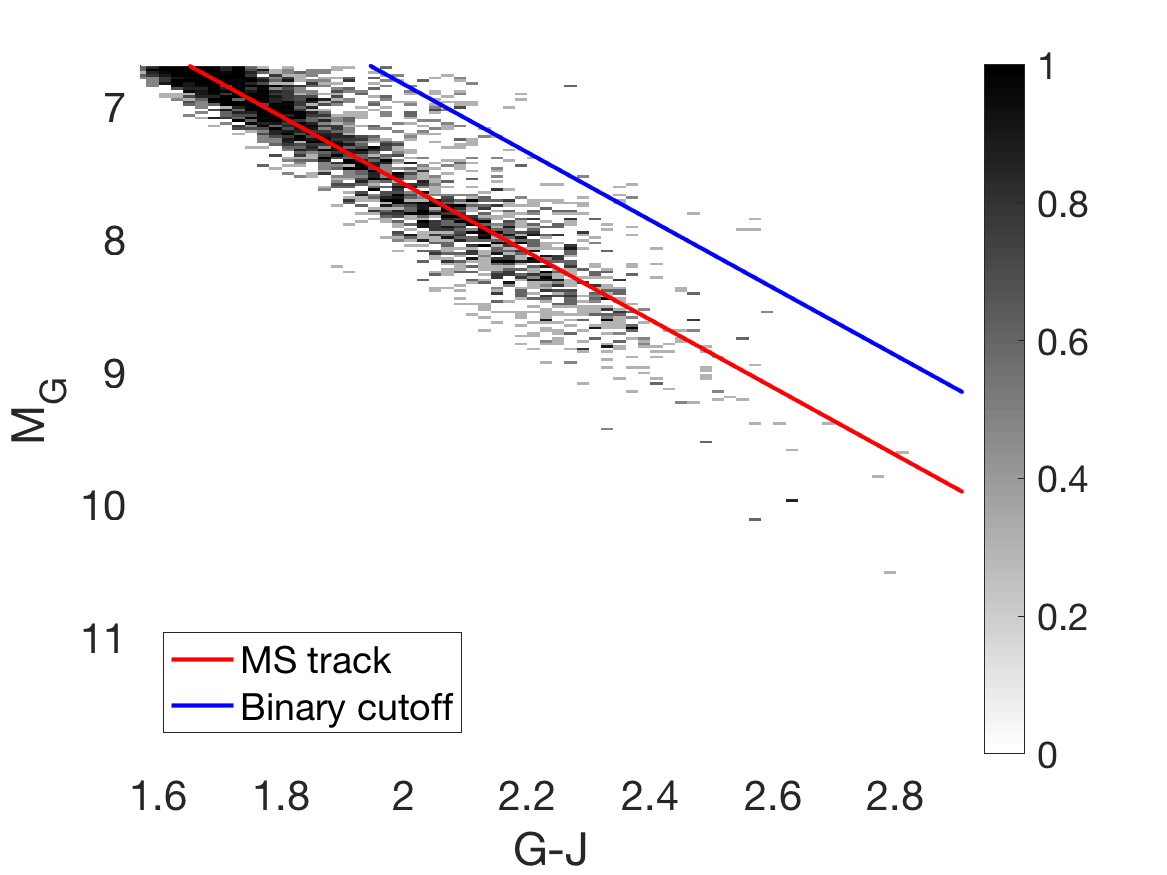
\includegraphics[width=0.8\textwidth]{Abs.png}
    \caption{An absolute colour-magnitude diagram for the combined sample of K- and M- dwarfs. The red line is the adopted best fit to the main sequence, while the blue line is the boundary used to separate the binary stars from the single-star systems.}
    \label{figGALAHbinary}
\end{figure}

\section{Absolute magnitude binning}
\label{secGALAHstack}
\begin{figure}
    \centering
    \captionsetup{width=.8\textwidth}
    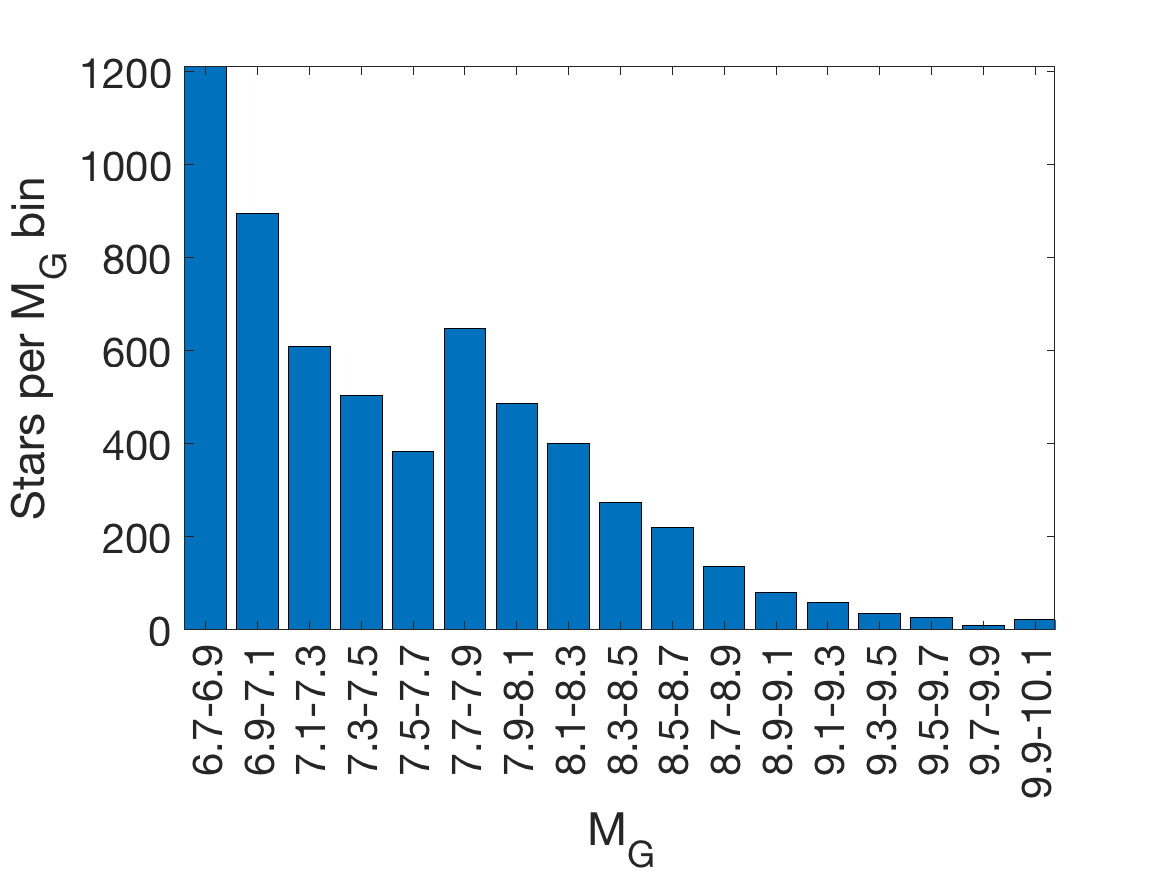
\includegraphics[width=0.8\textwidth]{GALAH_bin_histogram.png}
    \caption{The distribution of absolute magnitude for the sample of 
    GALAH M- and K- dwarfs.}
    \label{figGALAHhistogram}
\end{figure}

While the sample of GALAH M- and K- dwarfs contains a large number of observations, each star in the sample is typically observed only a few times at most. An ISV spectrum could be produced for each star in the same way as in Chapter \ref{chapISV}; however, this is too small a sample to produce a meaningful ISV spectrum for each star. This also means that a comparison of the ISV spectra produced from HARPS spectra and GALAH spectra for any star in both samples, is impossible without further GALAH observations. An alternative strategy was to produce ISV spectra from bins of observations from different, but structurally similar, stars. It is not unreasonable to expect that if the temperature range of each bin was sufficiently small, then the stars within the bin would be structurally similar, and therefore produce very similar spectra.\\

Absolute magnitude was used to segment the sample into 0.2-magnitude-wide bins, ranging from $M_G$\,=\,6.7 to 11.9. Figure\,\ref{figGALAHhistogram} presents the distribution of stars across the absolute magnitude bins. Bright bins contain hundreds of observations, with the population dropping steadily for intrinsically fainter stars. Using the minimum observation number of Chapter\,\ref{chapISV}, only bins with $\geqslant$20 observations were studied. This resulted in 16 useful bins across $M_G$\,=\,6.7-9.7 and 9.9-10.1. Plots of the median spectrum for each bin in the blue, green, red and infrared HERMES bandpasses are presented in Figures\,\ref{figGALAH_camera1}-\ref{figGALAH_camera4}, with the coolest stars at the top of each panel.\\

\begin{figure}
	\captionsetup{width=.8\textwidth}
	\hspace{-2cm}
	\subfloat[Blue]{\label{figGALAH_camera1}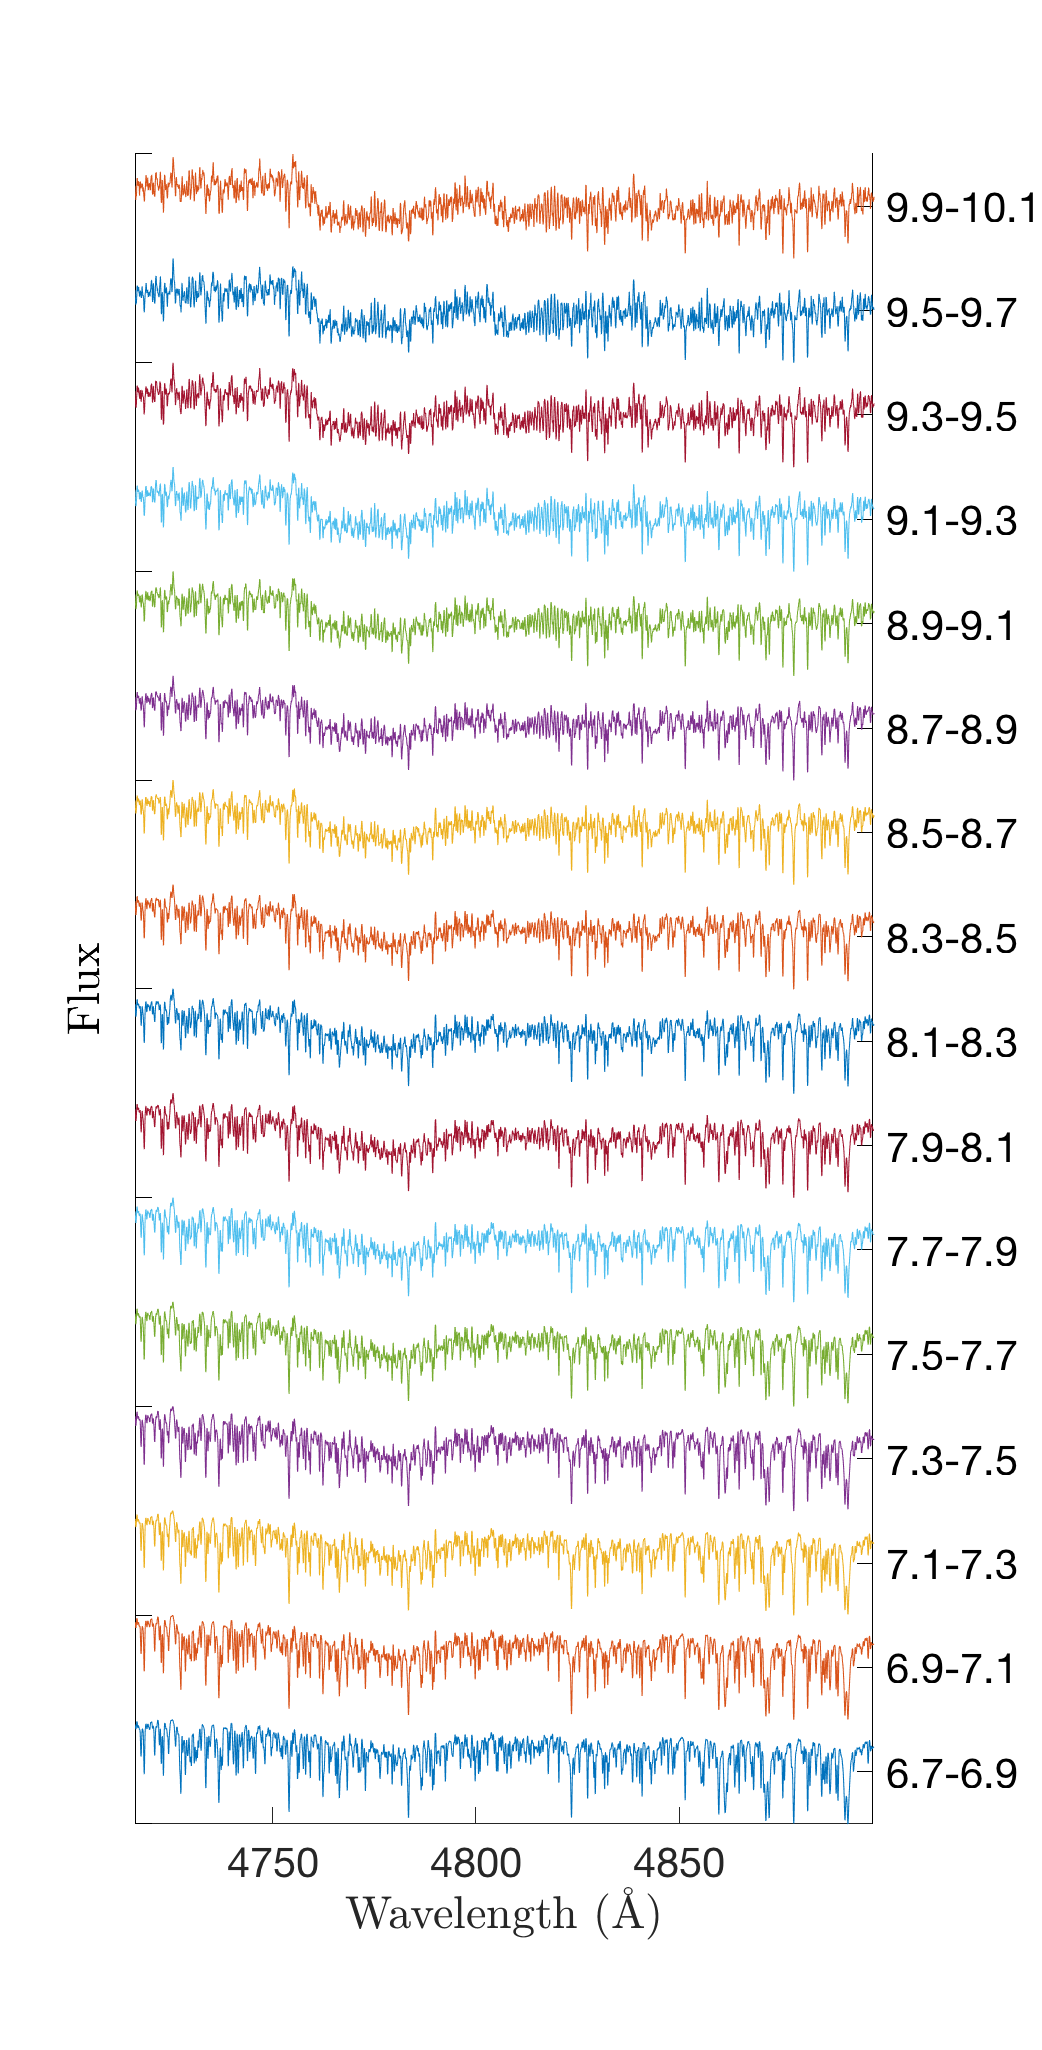
\includegraphics[width=0.6\textwidth]{GALAH_flux_camera_1.png}}
    \subfloat[Green]{\label{figGALAH_camera2}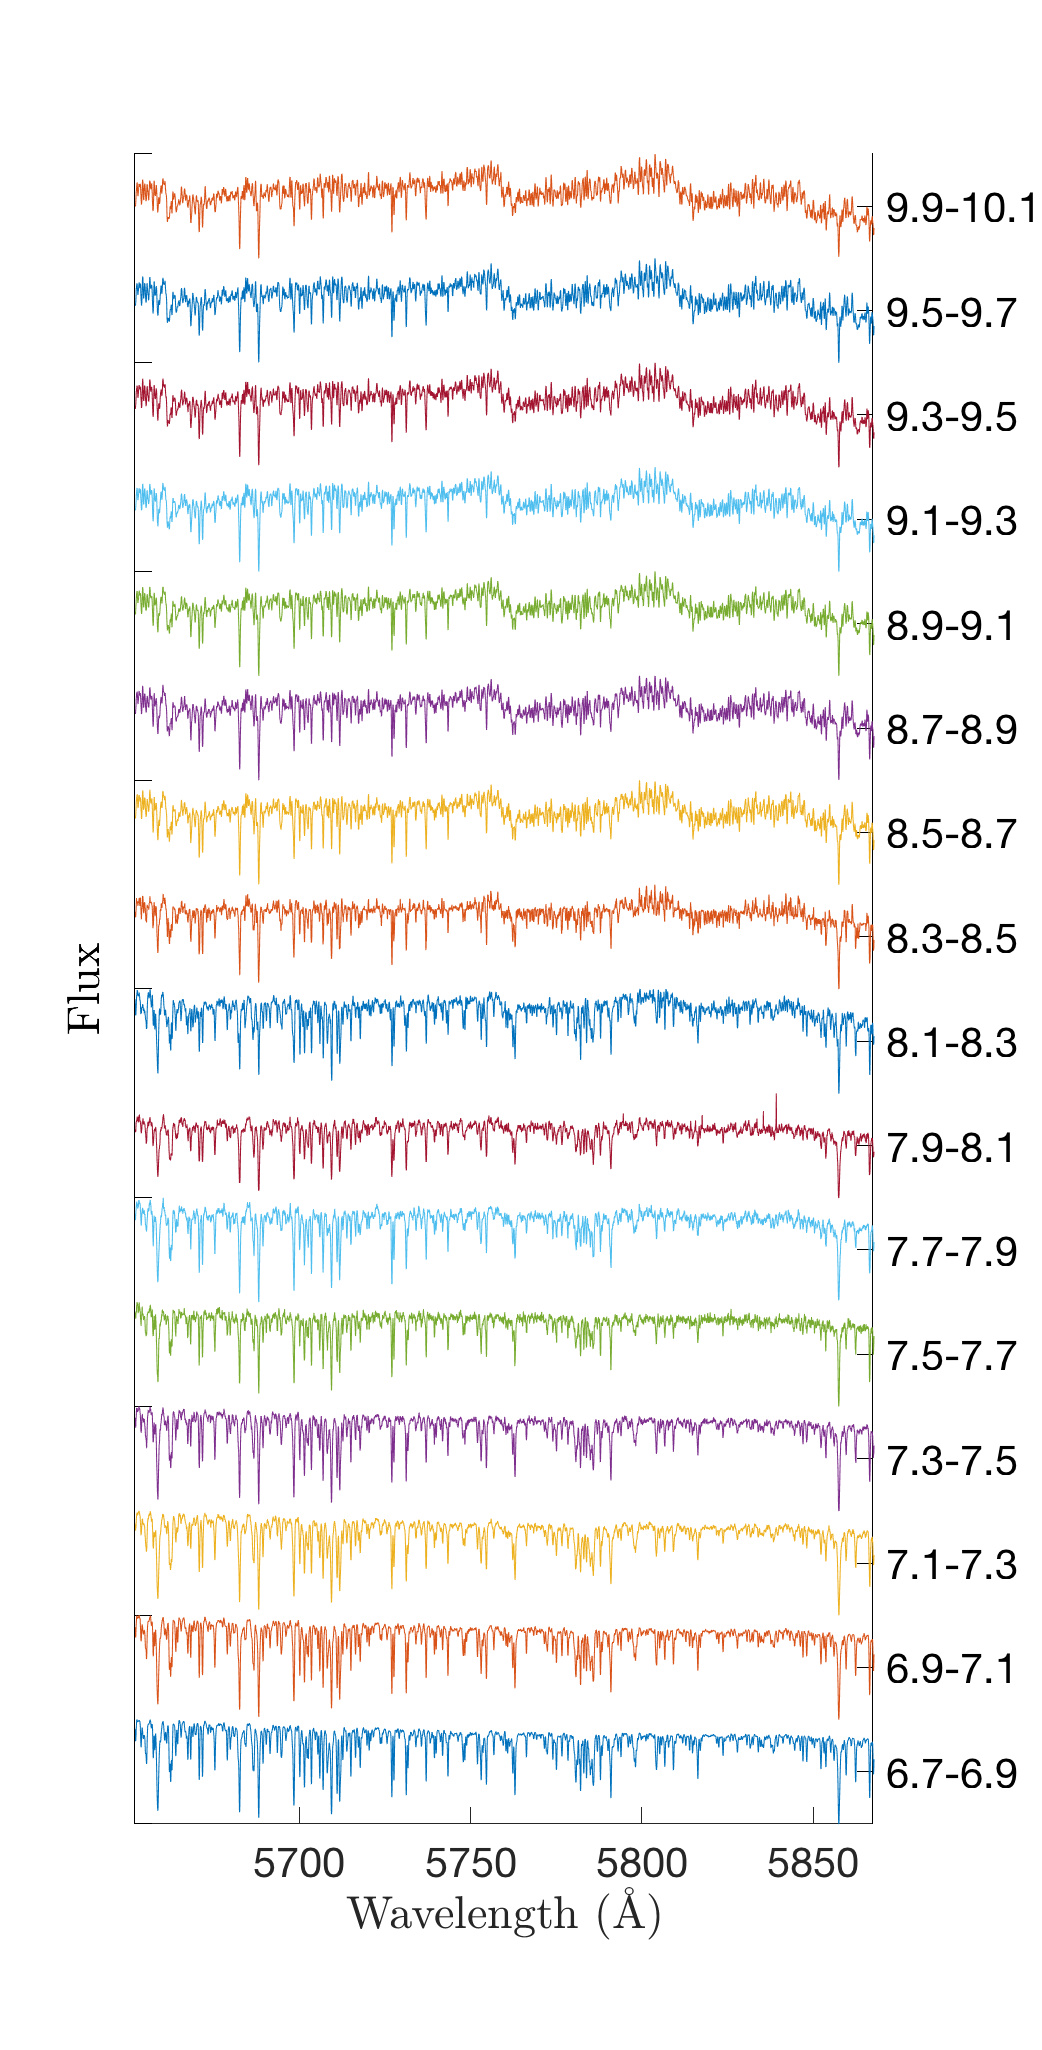
\includegraphics[width=0.6\textwidth]{GALAH_flux_camera_2.png}}\\
    \caption{Plots of the median spectra for each absolute magnitude bin. Each spectrum has been normalised and offset in the y-axis for visual clarity, and ranges from $M_G$\,=\,6.7-6.9 at the bottom, to $M_G$\,=\,9.9-10.1 at the top.}
\end{figure}
\begin{figure}
	\captionsetup{width=.8\textwidth}
	\hspace{-2cm}
    \subfloat[Red]{\label{figGALAH_camera3}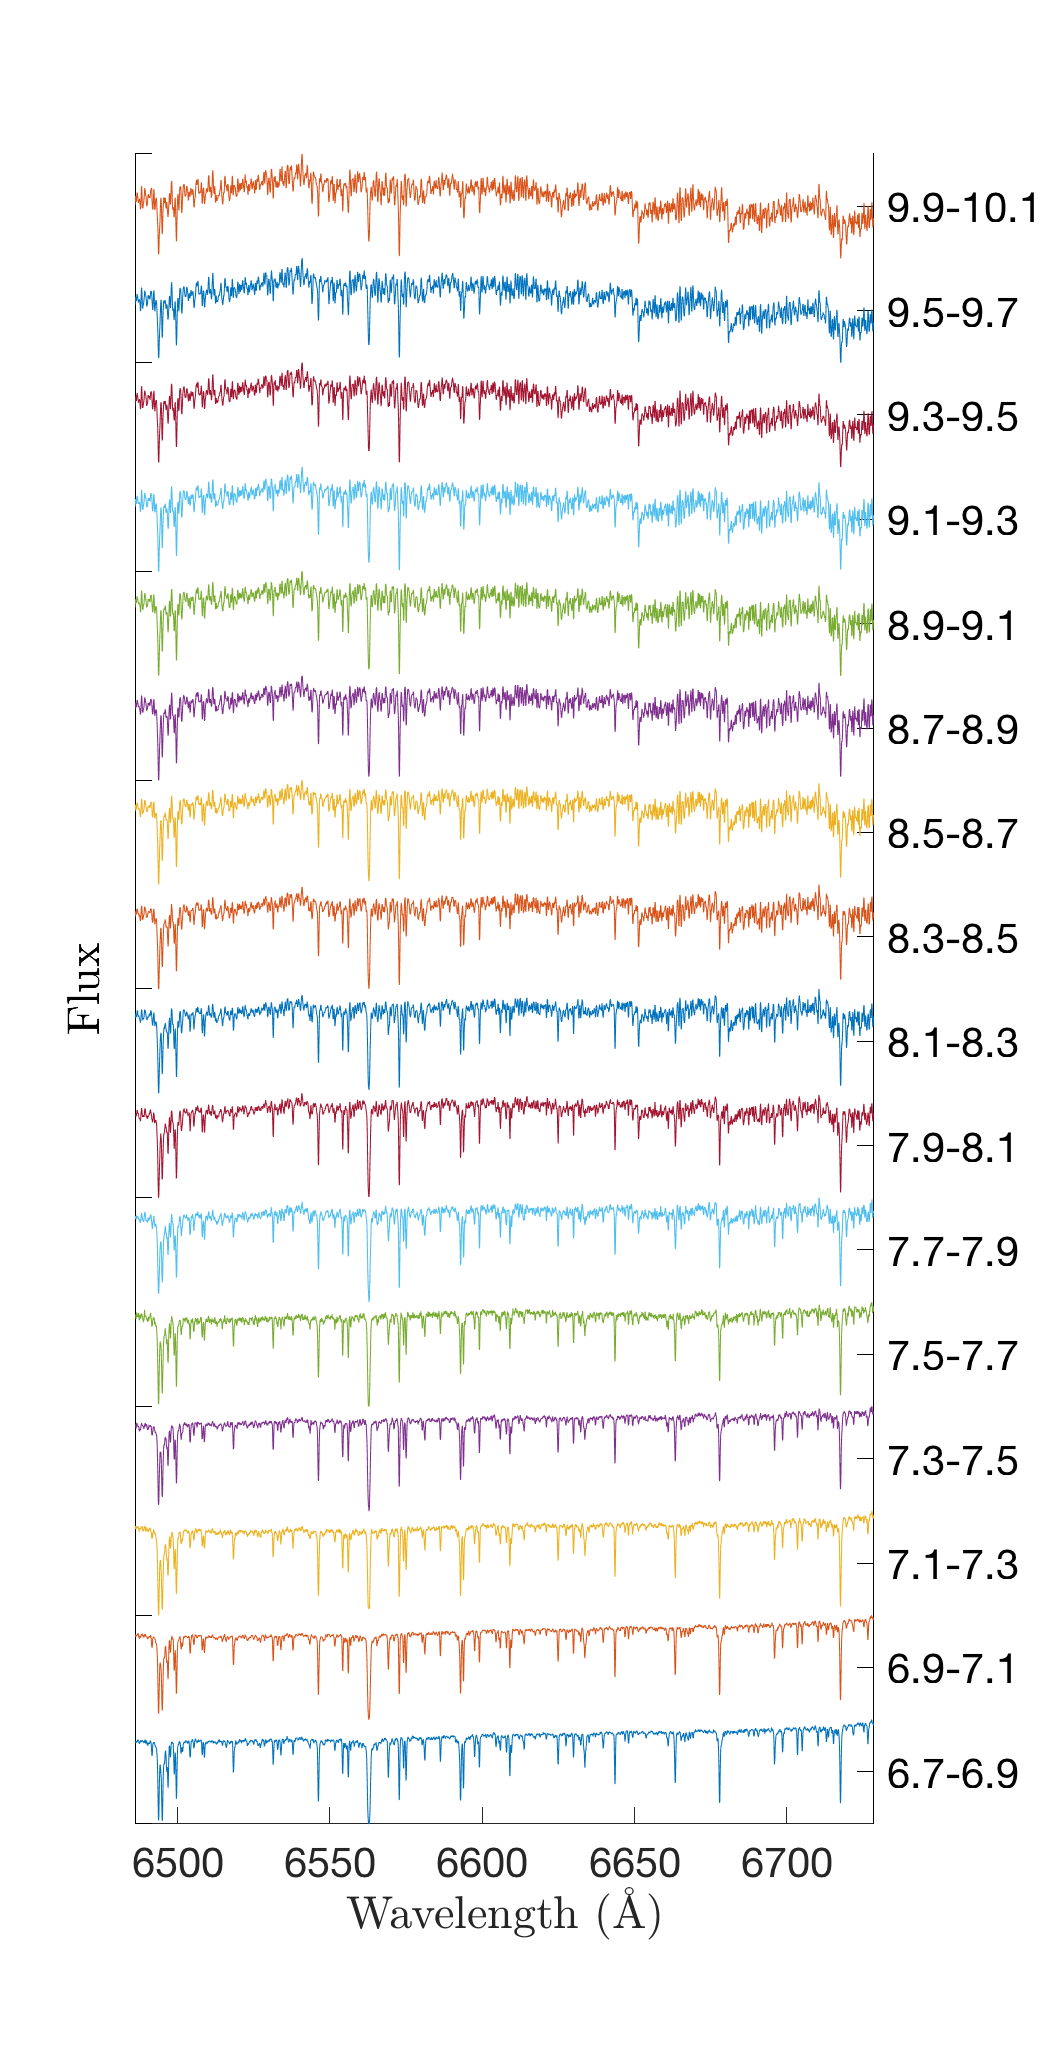
\includegraphics[width=0.6\textwidth]{GALAH_flux_camera_3.png}}
    \subfloat[Infrared]{\label{figGALAH_camera4}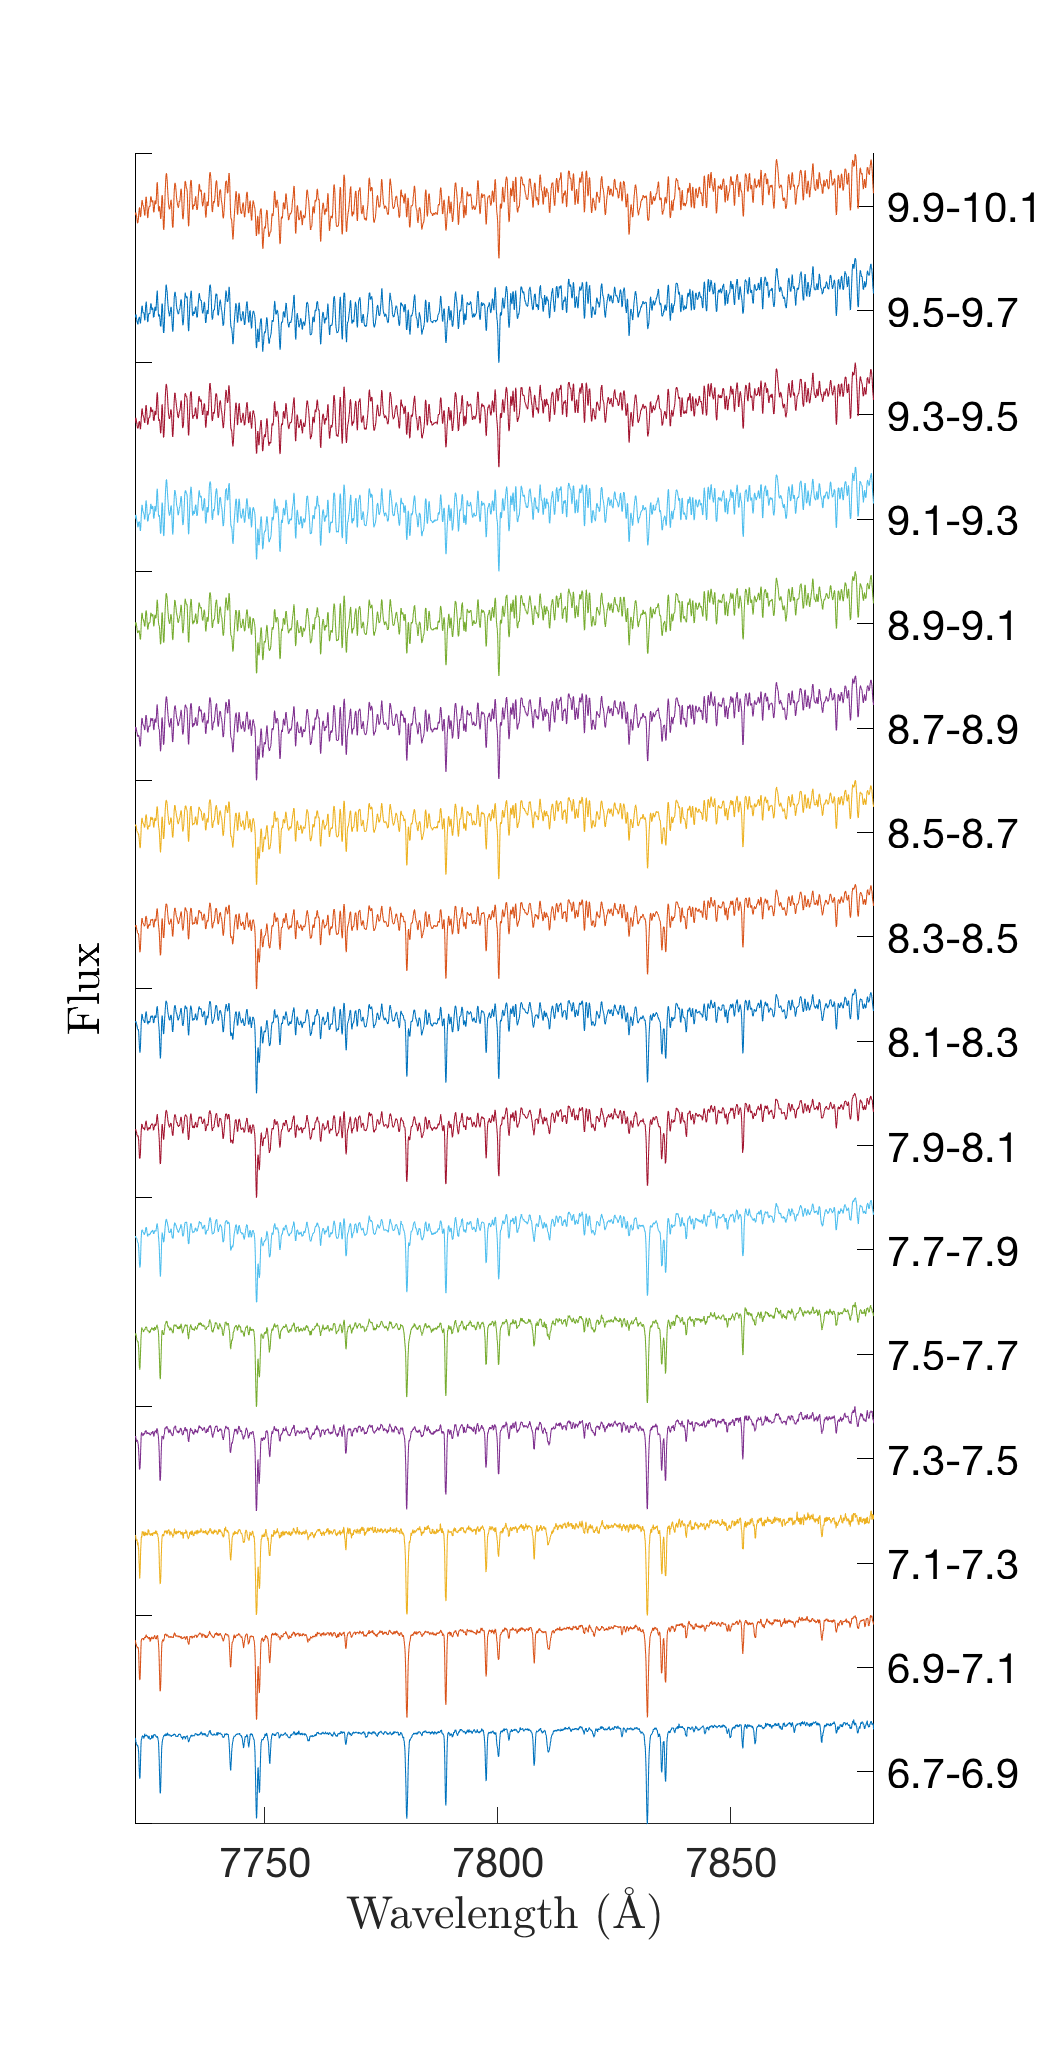
\includegraphics[width=0.6\textwidth]{GALAH_flux_camera_4.png}}\\
    \caption{Plots of the median spectra for each absolute magnitude bin. Each spectrum has been normalised and offset in the y-axis for visual clarity, and ranges from $M_G$\,=\,6.7-6.9 at the bottom, to $M_G$\,=\,9.9-10.1 at the top.}
\end{figure}

\section{GALAH-specific alterations to the ISV method}
\label{secGALAHalteration}
The ISV spectra produced from the GALAH data have characteristics not seen in HARPS ISV spectra. The magnitude of the baseline noise is significantly less than in the HARPS ISV, rarely exceeding a value of 1. This is both an advantage and disadvantage. Weak ISV lines that would have been buried in the baseline noise (if that noise was stronger) are more prominent in GALAH ISV spectra. This is a direct result of the large number of observations used to calculate the ISV spectra. Each HARPS star ISV spectrum was produced from tens to hundreds of observations, while the majority of the absolute-magnitude-limited GALAH subsamples contain significantly more observations. However, the low baseline noise and significant number of strong ISV lines make a 99.7th percentile threshold unhelpful. As discussed in Section\,\ref{secISVlines}, the distribution function for ISV spectra is assumed to be Gaussian, in which case the 99.7th percentile represents a 3$\sigma$ deviation from the mean. Using the red camera from the $M_G$\,=\,6.7-6.9 ISV spectrum as an example (Figure\,\ref{figGALAH_threshold_sigma}), it is clear that the 99.7th percentile (3$\sigma$; red dashed line) is higher than the majority of the ISV lines and using that level as a threshold would exclude a number of significant ISV lines. The 95.4th percentile (2$\sigma$; blue dashed line) was found to be a more suitable threshold for GALAH ISV spectra as it includes the majority of the visually obvious ISV lines, while maintaining a clear separation from the baseline noise.\\

\begin{figure}
    \centering
    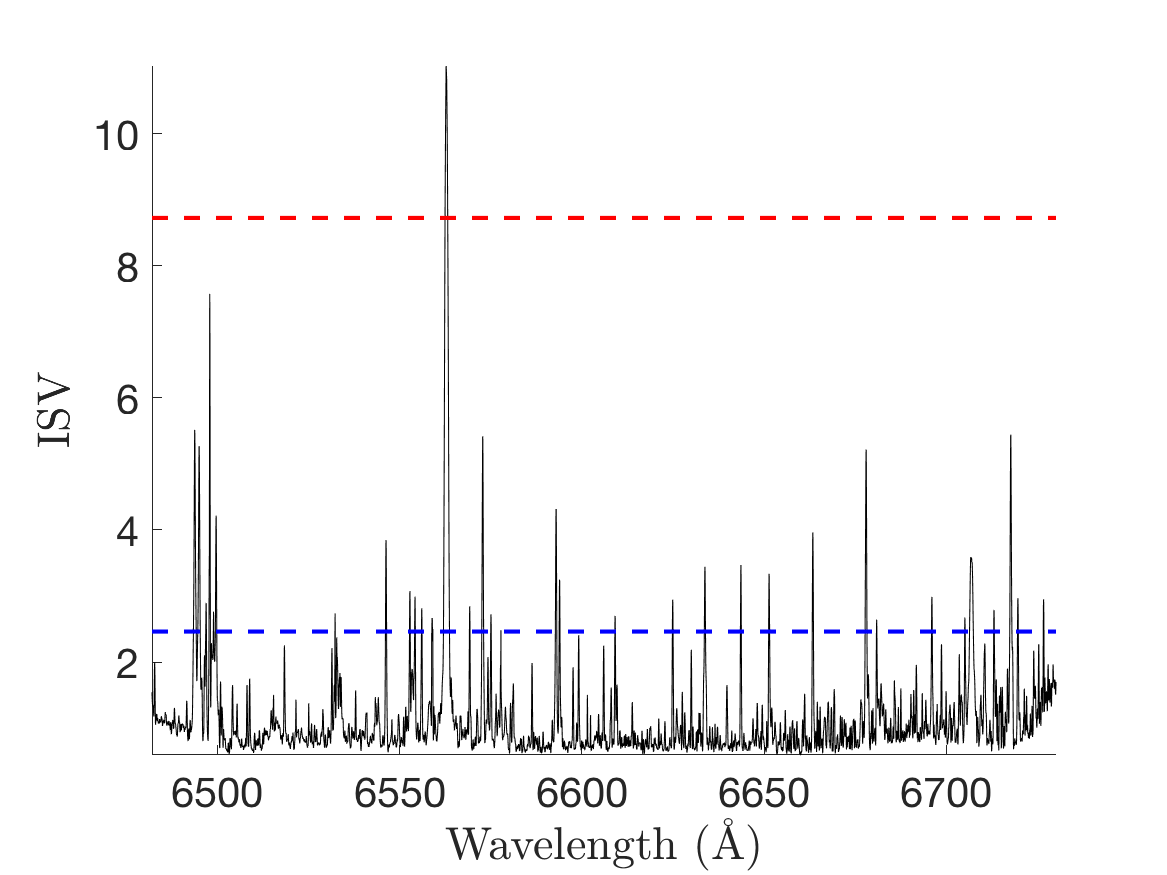
\includegraphics[width=.8\textwidth]{GALAHthresholdsigma.png}
    \caption{ISV spectrum of the $M_G$\,=\,6.7-6.9 bin for the red camera. The blue dashed line marks the 95.4th percentile, while the red dashed line is the 99.7th percentile.}
    \label{figGALAH_threshold_sigma}
\end{figure}

In the HARPS data, the threshold that ISV lines needed to exceed to be considered significant was calculated from the ISV spectrum of each star. For the GALAH data, an ISV spectrum is produced from spectra of stars within a specific range of absolute magnitude, and may well contain different features at different absolute magnitudes. Therefore a separate threshold is required for each absolute magnitude bin. Figure\,\ref{figGALAH_threshold_global} highlights how the baseline noise and the ISV lines selected by this threshold vary between cameras. If the threshold is calculated from a 95.4th percentile of the ISV spectra of all four cameras together, the threshold (blue dashed line) is too high for the blue camera (i.e. it is higher than most of the ISV lines), and too low for the infrared camera (i.e. it is too close to the baseline noise). Instead of a `global' threshold, a 95.4th percentile threshold was adopted for each camera individually. The resulting threshold for each camera is a better representation of the baseline noise and the ISV lines for that camera, and is plotted as the red dashed lines in Figure\,\ref{figGALAH_threshold_global}. In summary, the thresholds were determined on a per absolute magnitude bin and per camera basis.\\

\begin{figure}
    \hspace{-2cm}
    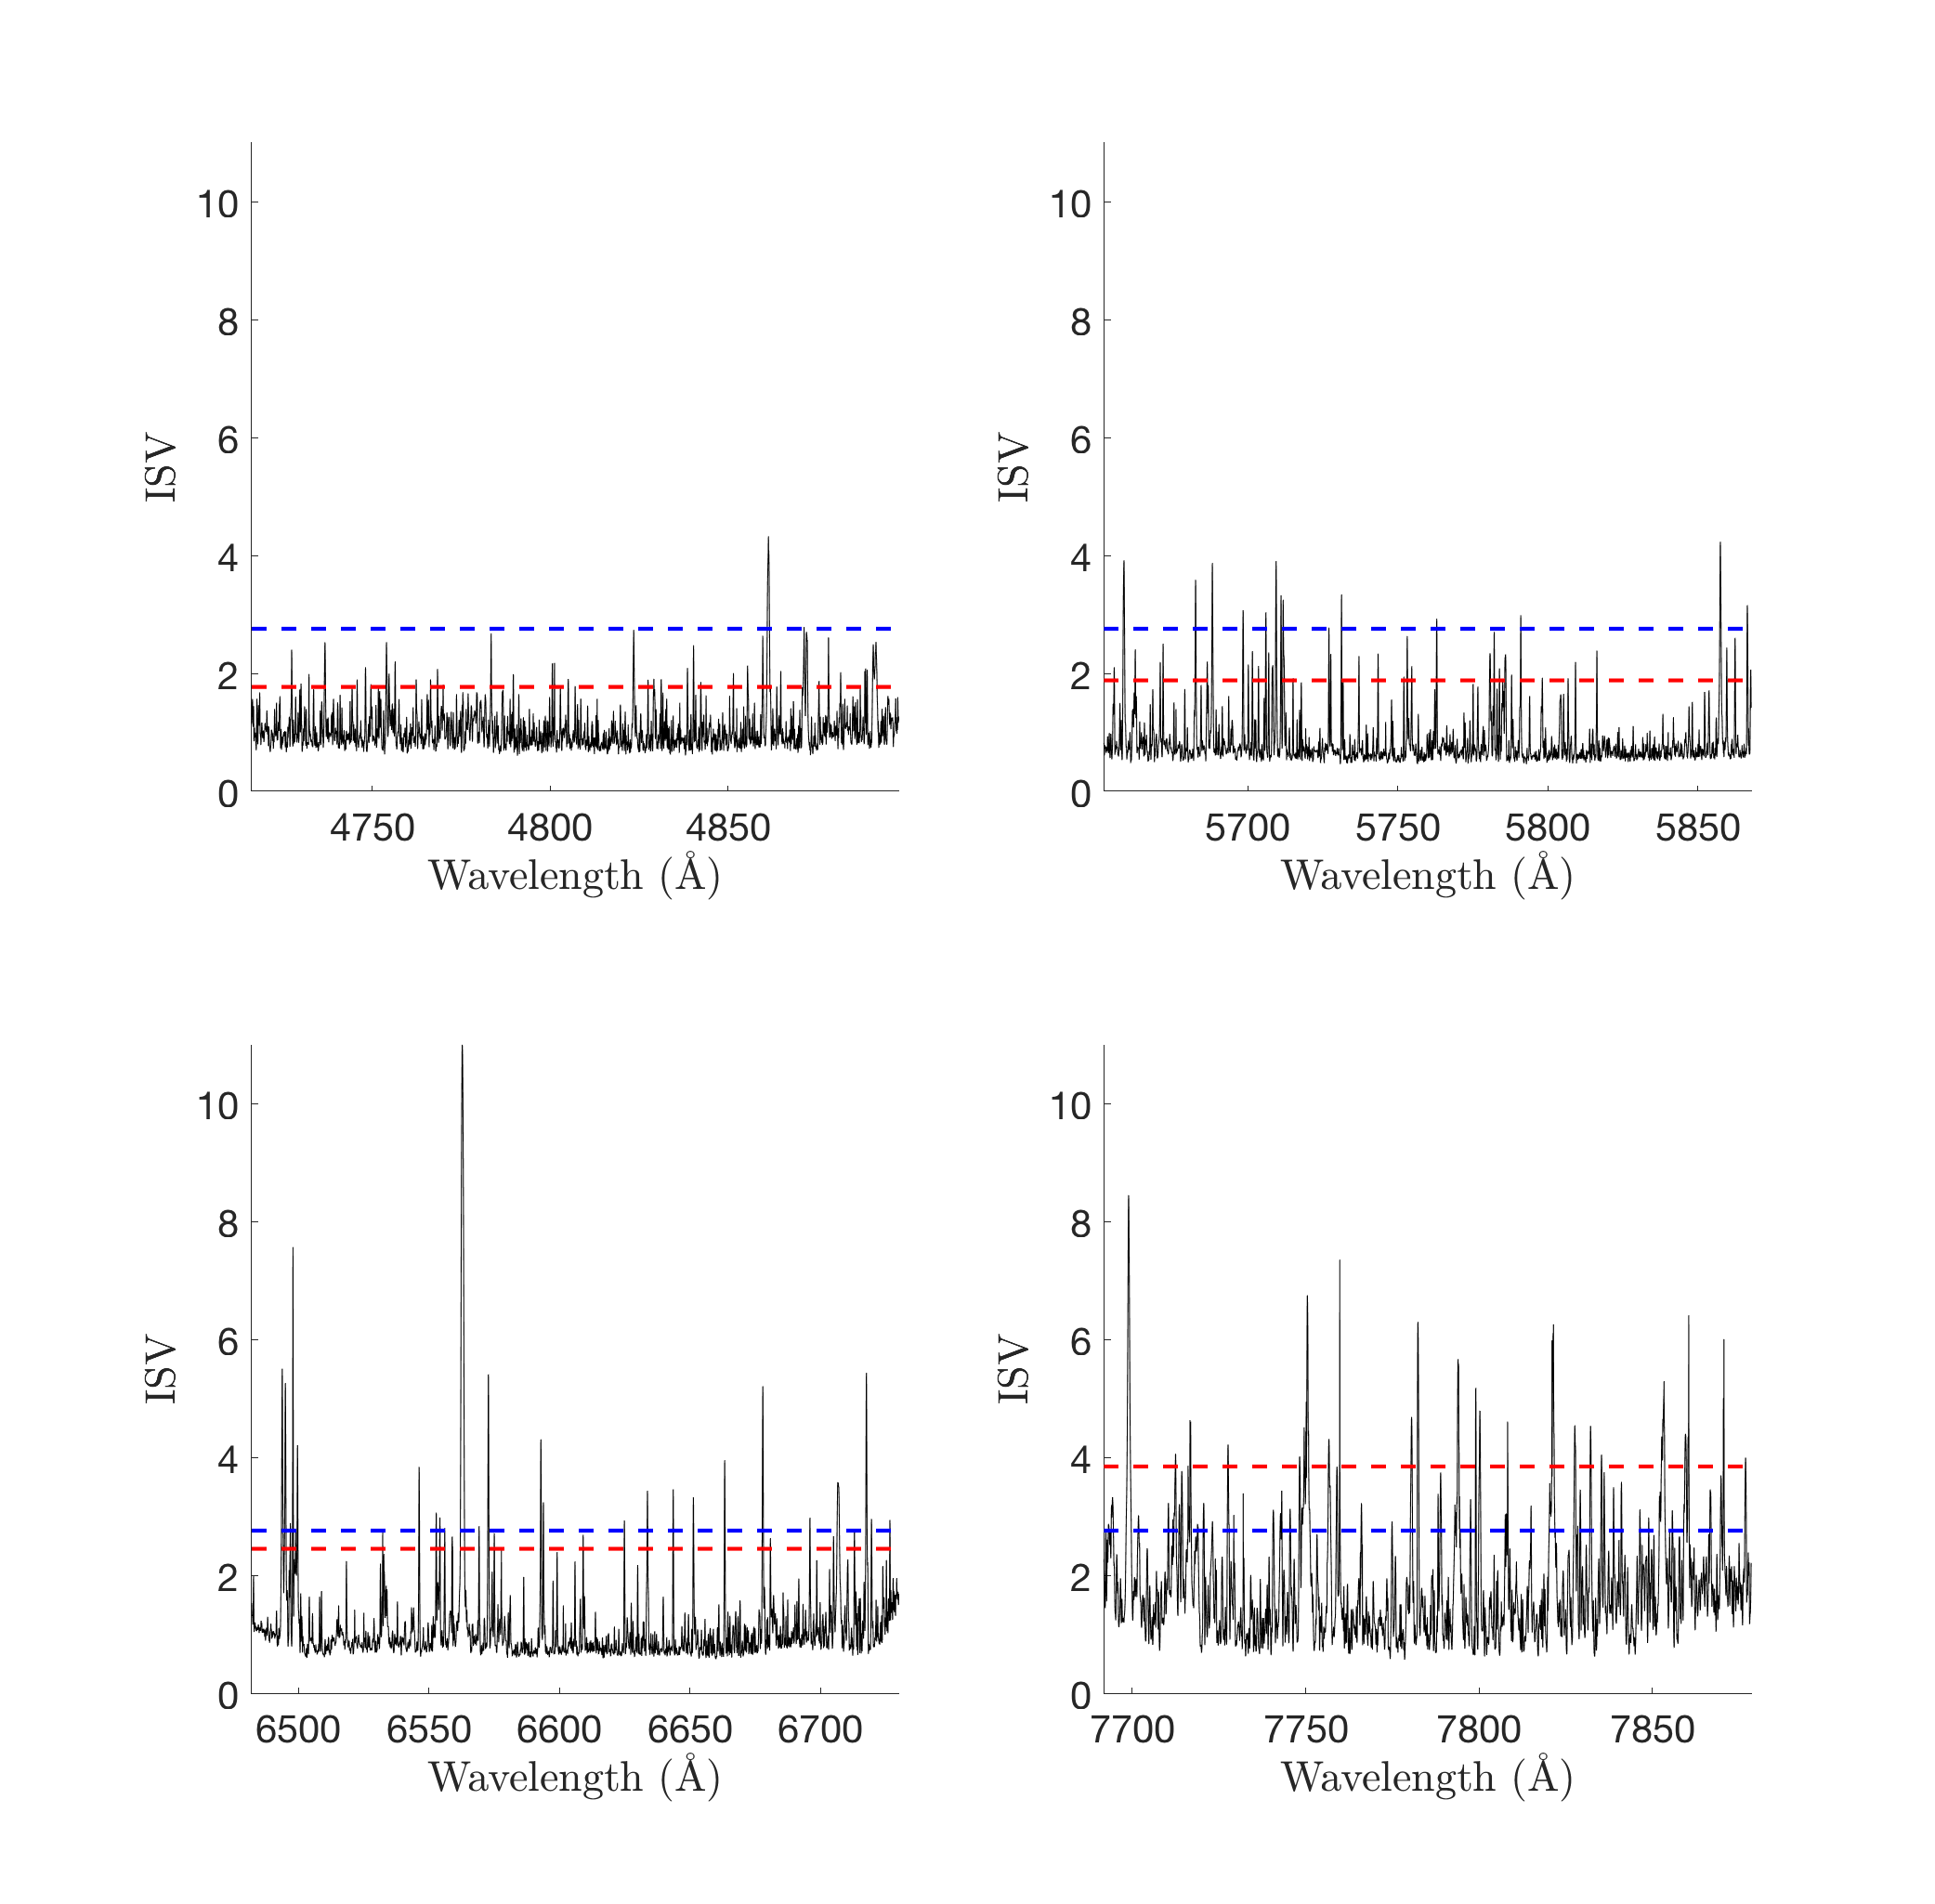
\includegraphics[width=1.2\textwidth]{GALAHthresholdglobal.png}
    \caption{ISV spectra of the $M_G$\,=\,6.7-6.9 bin for each camera. The blue dashed line represents the threshold using the ISV from all cameras together. The red dashed line represents the threshold for each individual camera.}
    \label{figGALAH_threshold_global}
\end{figure}

HARPS ISV spectra have a resolution of 0.06\hbox{\AA}, allowing individual ISV lines to be fully resolved and making it straightforward to identify and measure their strength. The observations that produced each ISV spectrum were of the same star, so the only differences from observation to observation were in the total amount of flux collected, photon noise, seeing, and stellar variability.\\

In contrast, GALAH ISV spectra are constructed from multiple observations in narrow absolute magnitude ranges. Although the size of each absolute magnitude bin was kept small, the stars in each bin will not have {\em exactly} the same stellar structure or abundance patterns. This will produce variation in the ISV spectrum for that bin not from a time-varying spectral line, but from the small differences in the spectra from star to star. In addition, the lower resolution of the HERMES spectrograph (R=28,000) relative to HARPS (R=125,000), will produce ISV lines that are broader than in the HARPS ISV spectra. In some cases multiple lines may overlap, making it difficult to resolve them individually in the ISV spectrum.\\

Figure\,\ref{figresolve} compares 10\hbox{\AA} regions from HARPS and GALAH ISV spectra. (There is little wavelength overlap between HARPS and GALAH, and there are no lines of significance in that overlap, so a common wavelength range was not selected.) The two ISV lines in the HARPS ISV spectrum of Figure\,\ref{figHARPSresolve} are separated by several \hbox{\AA} and are typically around 0.2\hbox{\AA} wide. A GALAH ISV spectrum contains lines with a typical width of 1.4\hbox{\AA} and can contain regions similar to what is seen in Figure\,\ref{figGALAHresolve}, where five lines cannot be fully resolved back to the baseline noise level. This is problematic as the original method for measuring the magnitude of an ISV line, $A_{ISV}$, uses the full range of wavelengths above the baseline noise comprising the ISV line. Unresolved ISV lines will contain overlapping wavelengths that are the combination of the variation in each line. Disentangling the contribution of each line in an overlapping region would be difficult. In these cases, the limits of the wavelength range corresponding to the ISV line were determined as the lowest point in the overlap region (i.e. the wavelength at which the gradient of the ISV spectrum changes from negative to positive).\\

\begin{figure}
	\captionsetup{width=.8\textwidth}
	\subfloat[HARPS]{\label{figHARPSresolve}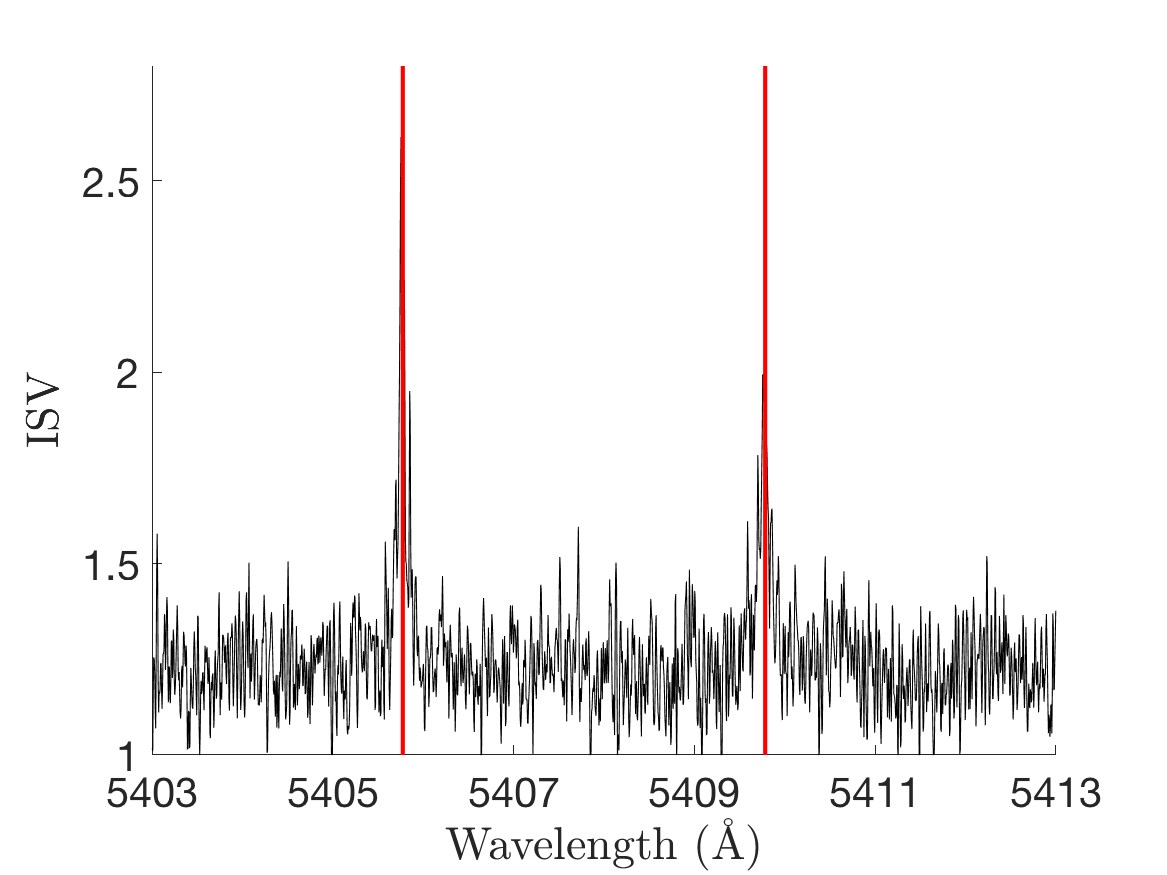
\includegraphics[width=0.5\textwidth]{HARPSunresolved.png}}
    \subfloat[GALAH]{\label{figGALAHresolve}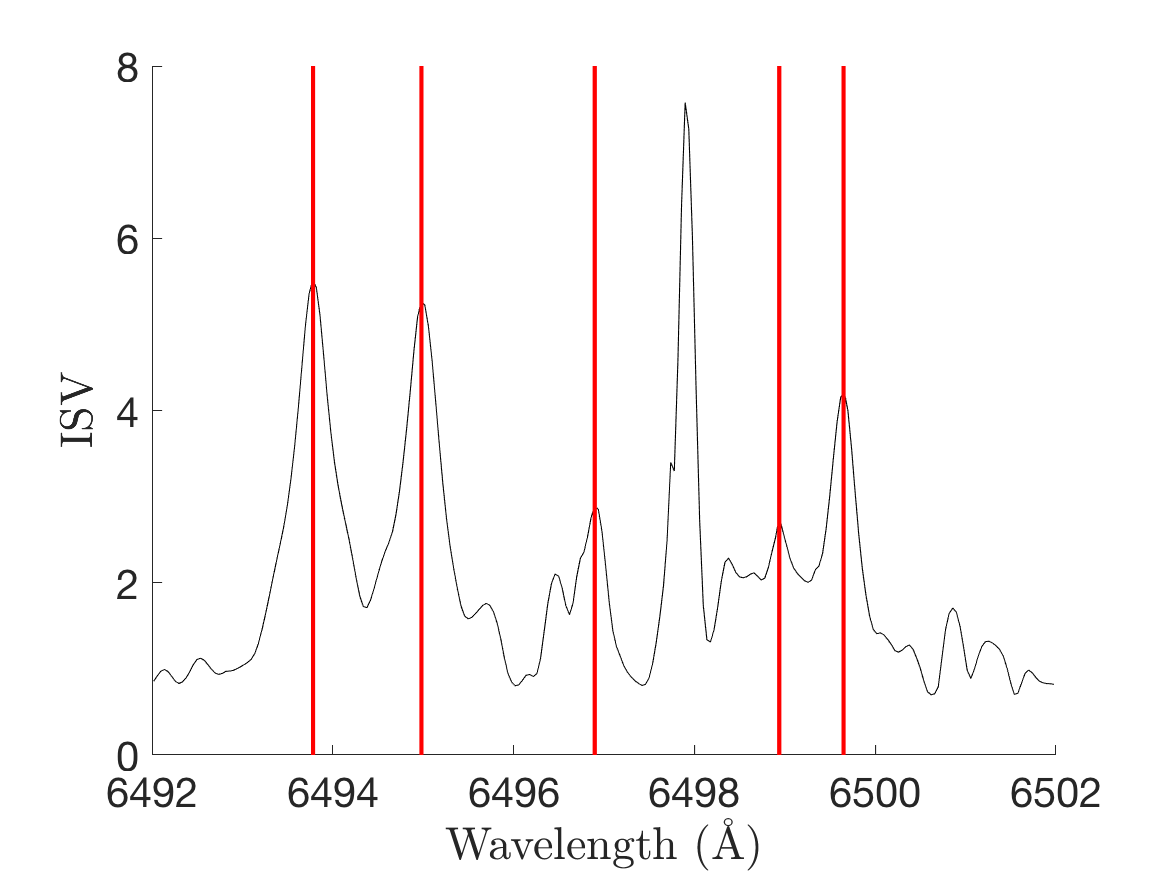
\includegraphics[width=0.5\textwidth]{GALAHunresolved.png}}
    \caption{ISV spectra from HARPS (left) and GALAH (right). The vertical red lines indicate known spectral lines from the line list used in this work.}
    \label{figresolve}
\end{figure}

In addition, the signal-to-noise of the baseline noise around the ISV line will be harder to determine if the lines are unresolved. The signal-to-noise was determined in Chapter\,\ref{chapISV} using 40 pixels on either side of the ISV line; however, in situations like what is seen in Figure\,\ref{figGALAHresolve} where there are overlapping ISV lines, the 40 pixels will include nearby ISV lines, resulting in a false determination of the uncertainty of the $A_{ISV}$. Instead the signal-to-noise was measured using the baseline noise in the ISV across the entire camera. The signal-to-noise for each ISV line was determined as the mean ISV value across the ISV line divided by the standard deviation of all points in the camera that fall below the 95.4th percentile threshold. From Figures\,\ref{figGALAH_ISV_camera1}-\ref{figGALAH_ISV_camera4} it can be seen that (with the exception of the infrared camera) the baseline noise does not change significantly across a bandpass, so a signal-to-noise determined from the ISV spectrum across the entire camera should be a reasonable estimate of the signal-to-noise at any individual ISV line.\\

The last adjustment to the ISV algorithm for GALAH data concerns the minimum resolvable element in each spectrum. An ISV spectrum will contain ISV lines produced by varying spectral lines, and it may also contain cosmic rays not removed in the data reduction process or artifacts produced in the making of the ISV spectrum. Any ISV line narrower than the minimum resolvable element of the spectrograph will not be the product of a varying spectral line and can be ignored. For the resolution of the spectrograph, and the wavelength range used, the HARPS minimum resolvable element ranged from 0.04\hbox{\AA} to 0.06\hbox{\AA} (see Section\,\ref{secISVdataprep}), with the latter being used as the minimum width allowable for an ISV line. For GALAH this value ranges from 0.17\hbox{\AA} at the start of the blue camera to 0.28\hbox{\AA} at the end of the infrared camera. However, there is significant wavelength spacing between each camera, so the minimum resolvable element varies substantially between cameras. The values used for the blue, green, red, and infrared cameras were 0.18, 0.21, 0.24, and 0.28\hbox{\AA} respectively.

\section{Telluric absorption and atmospheric emission lines}
\label{secGALAHnonstellar}
The GALAH data reduction pipeline includes the identification and removal of terrestrial features from the spectrum. However, this process can sometimes miss terrestrial features that could produce ISV variation. To study the potential presence of any missed telluric features, and to investigate their impact on the ISV spectra, an exploration similar to that of Section\,\ref{secNonStellarLines} was carried out.\\  

The photometric selection method was used to obtain the colour and absolute magnitude ranges required to identify a sample of GALAH B-dwarfs (Table\,\ref{eqBD}). This resulted in 5,691 observations that underwent the same preparation as the spectra of HD148605 for the HARPS data to produce an ISV spectrum (see Section\,\ref{secNonStellarLines} for details). To ensure the baseline noise in the ISV was minimal, the spectroscopic signal-to-noise cut used was 200 per pixel in all cameras. The spectra were then visually inspected, and spectra exhibiting narrow H$\alpha$ and H$\beta$ lines, indicating low v$sin(i)$, were removed. The remaining subsample comprised 39 observations.\\

As with the HARPS B-dwarfs, these spectra would be difficult to precisely velocity correct because of their lack of sharp features. Similar to the M-dwarfs and K-dwarfs, to ensure a consistent velocity zeropoint, a template B-star spectrum was selected, barycentrically corrected, and the rest were cross-correlated to it to better align the spectra.\\

\begin{table}[]
    \centering
    \begin{tabular}{|r|}
        \hline
        GALAH B-star phoometric selection criteria\\
        \hline
		M$_G$\,\textgreater\,0\\
		M$_G$\,\textless\,1\\
        K-W2\,\textgreater\,-0.08\\
        K-W2\,\textless\,0.04\\
        G-K\,\textgreater\,-0.3\\
        G-K\,\textless\,0.4\\
    	G-J\,\textgreater\,-0.2\\
    	G-J\,\textless\,0.3\\
    	J-K\,\textgreater\,-0.1\\
    	J-K\,\textless\,0.1\\
		W1-W2\,\textgreater\,-0.1\\
    	W1-W2\,\textless\,0.03\\
        \hline
    \end{tabular}
    \caption{Colour selection to identify the GALAH B-star sample.}
    \label{eqBD}
\end{table}


The original spectra, aligned spectra, and resulting ISV spectra for GALAH B-dwarfs can be seen in Figure\,\ref{figGALAH_B_1}-\ref{figGALAH_B_4}. Unlike the ISV of HD148605 (Figure\,\ref{figHD148605_ISV}), the baseline of the ISV is not flat. This is due to significant differences in the profile of the spectrum around the strong H$\beta$ and H$\alpha$ lines present in the blue and red cameras (respectively). Investigation of the spectra, both pre- and post- velocity correction, and the ISV produced, found no wavelengths outside of the A band at which sky absorption was significant (i.e. there were no narrow absorption lines that were found to be aligned in the original spectra, but misaligned in the velocity corrected spectra). While the GALAH data reduction pipeline was mostly successful at correcting telluric features in the spectra, the saturated parts of the Fraunhofer A-band at 7600\hbox{\AA} are difficult to remove completely. It was decided to remove the wavelengths containing this feature, regardless of whether the telluric correction was successful, by removing all data in the infrared camera blueward of 7723\,\hbox{\AA}.\\  

\begin{figure}
	\captionsetup{width=.8\textwidth}
	\hspace{-2cm}
    \subfloat[Blue]{\label{figGALAH_B_1}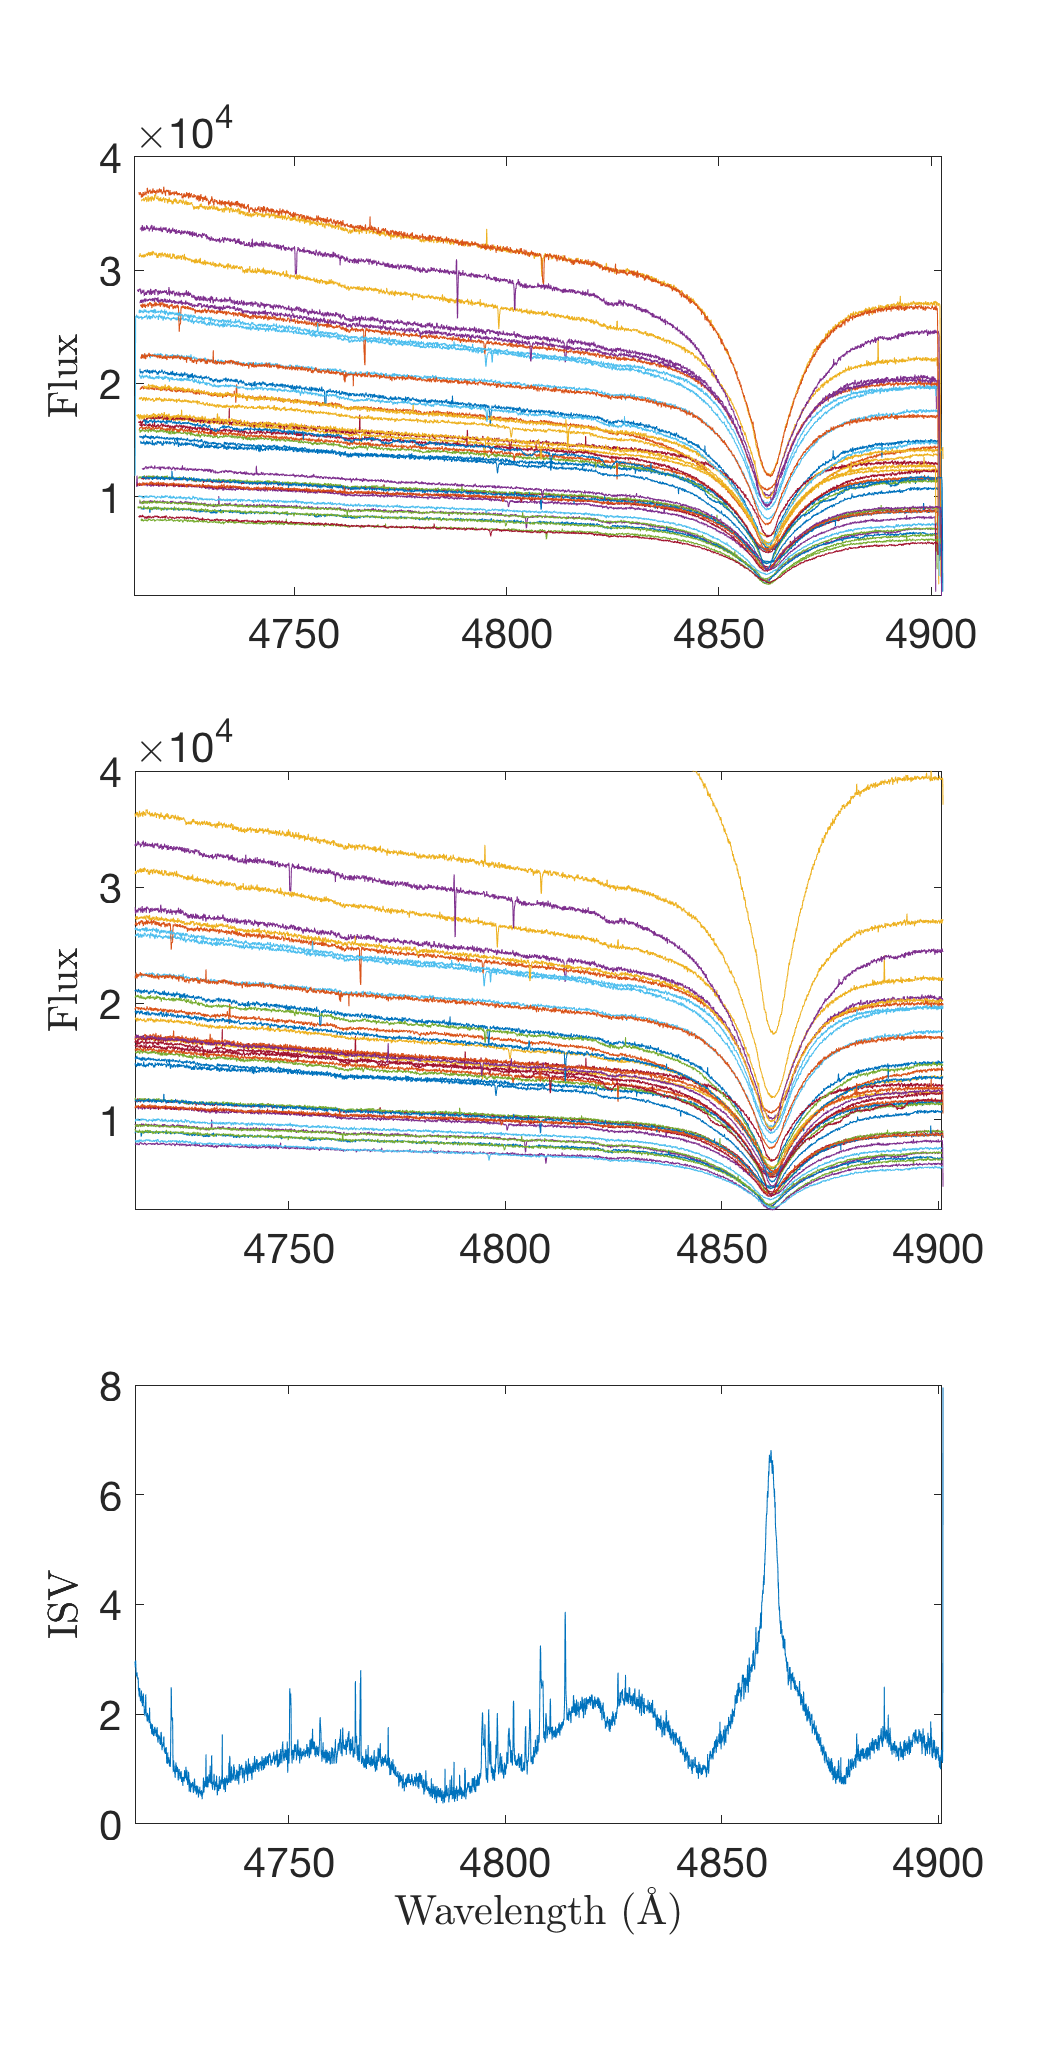
\includegraphics[width=0.6\textwidth]{GALAH_B_1.png}}
    \subfloat[Green]{\label{figGALAH_B_2}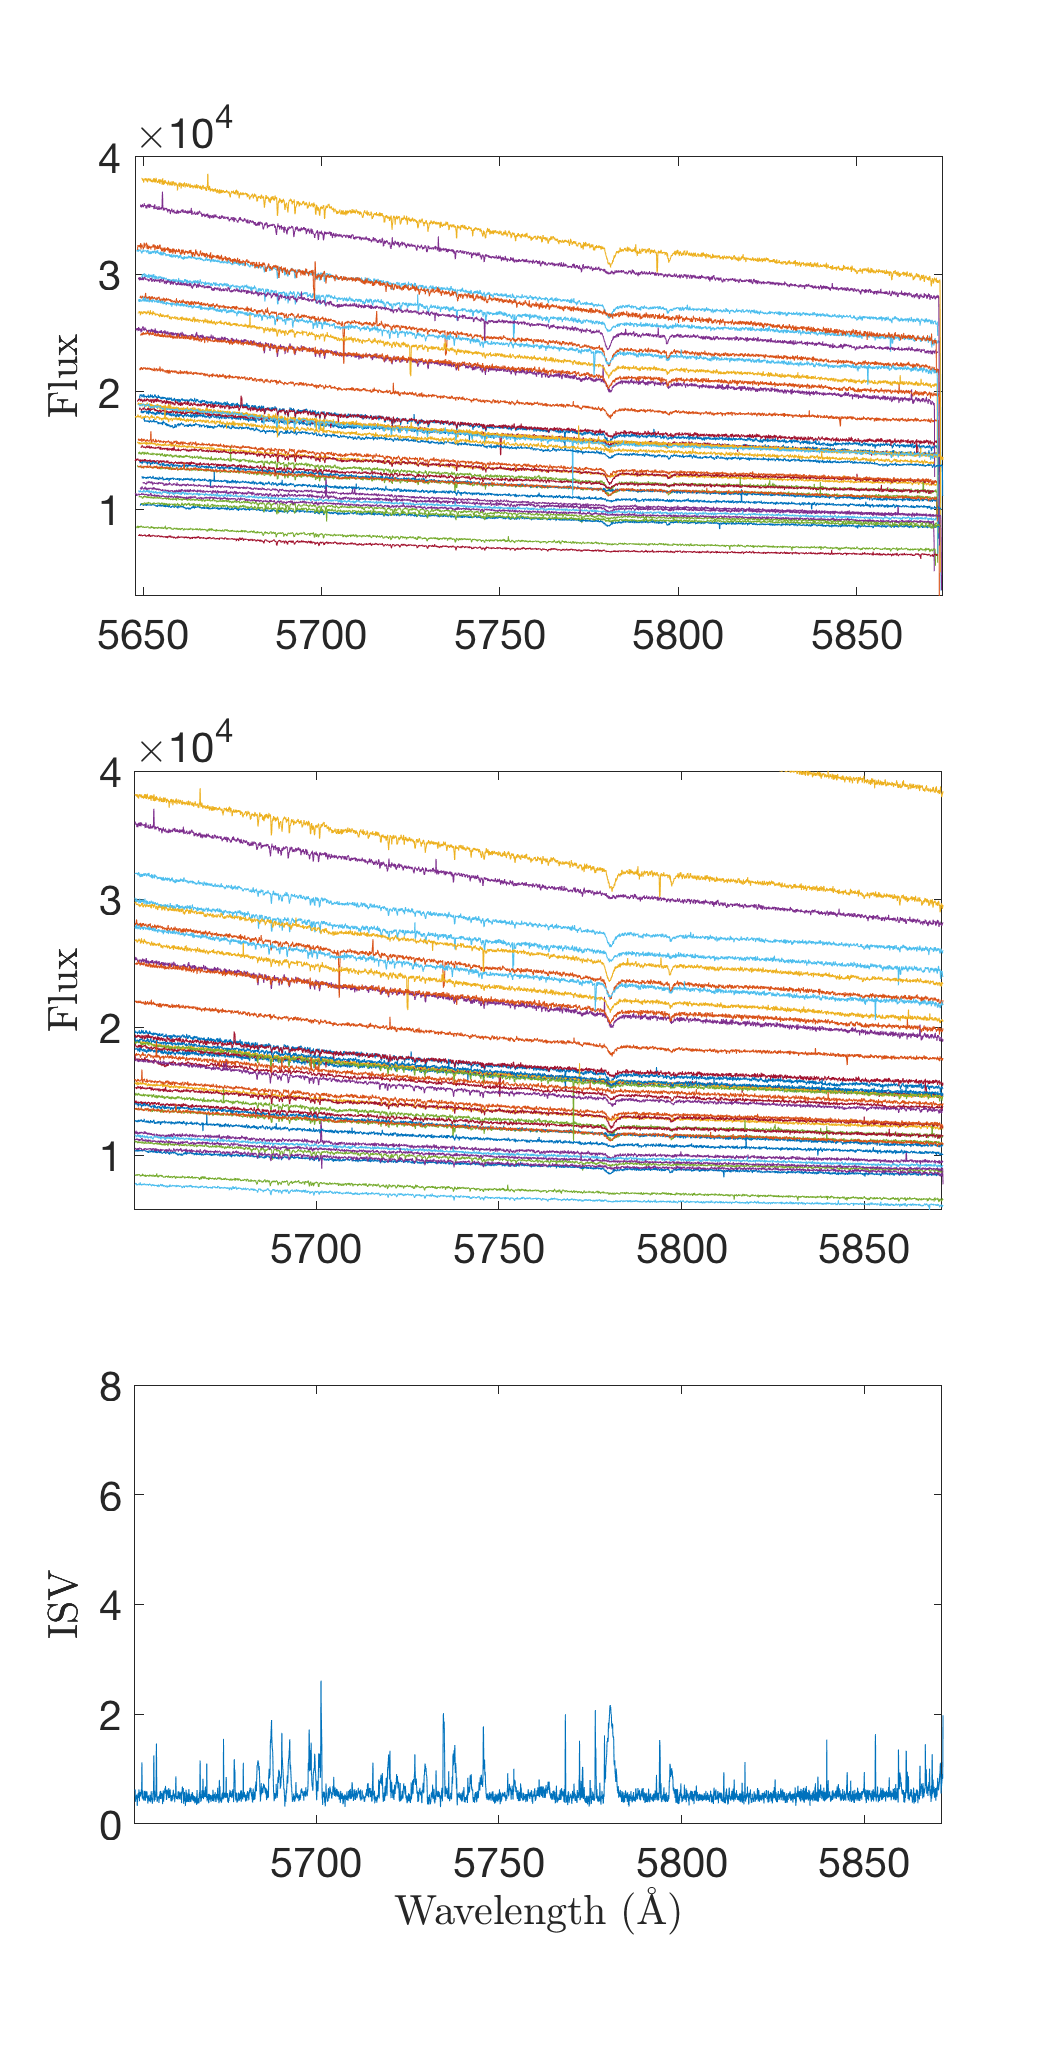
\includegraphics[width=0.6\textwidth]{GALAH_B_2.png}}
    \caption{(Top) GALAH spectra of 39 B-dwarfs. (Middle) The spectra once aligned onto the same wavelength scale. (Bottom) The ISV spectrum produced from the aligned spectra.}
    \label{figGALAHbstar1}
\end{figure}
\begin{figure}
	\captionsetup{width=.8\textwidth}
    \hspace{-2cm}
    \subfloat[Red]{\label{figGALAH_B_3}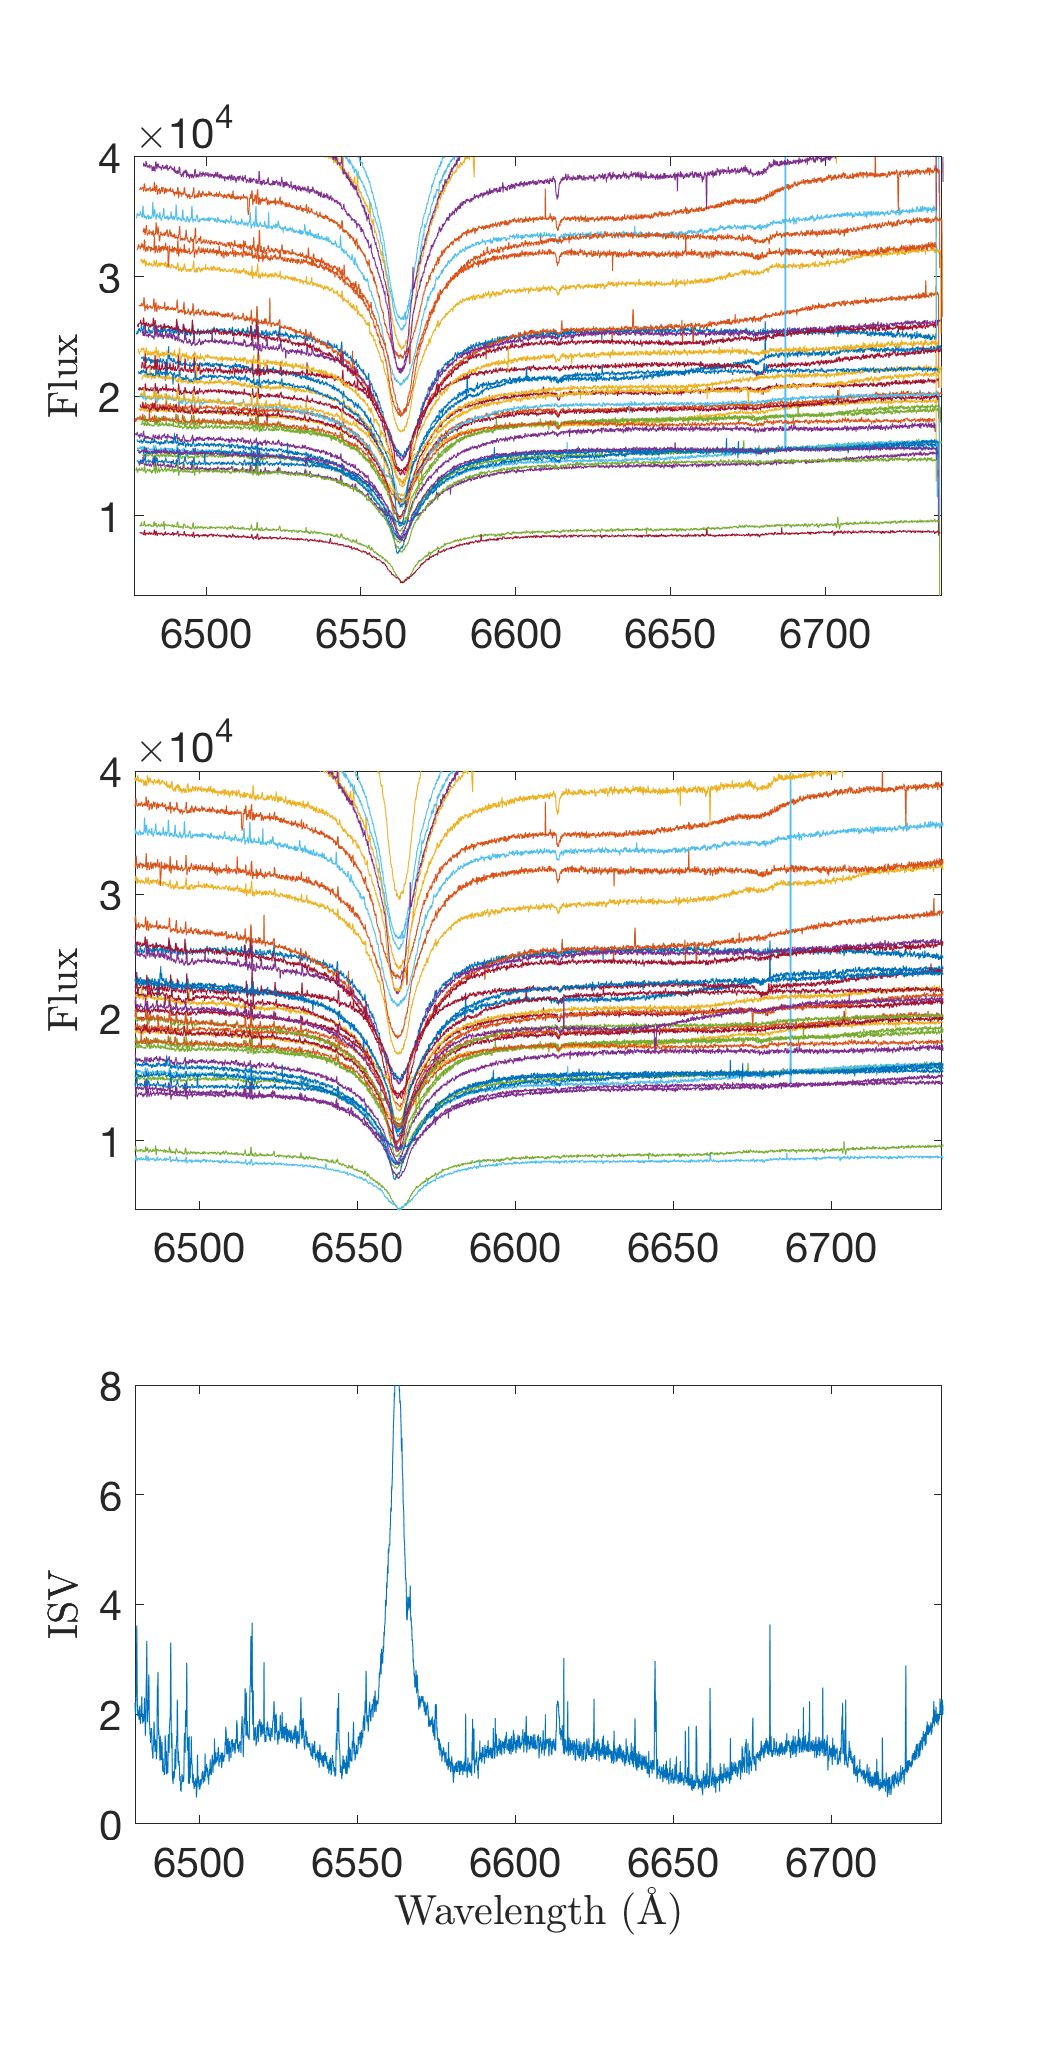
\includegraphics[width=0.6\textwidth]{GALAH_B_3.png}}
    \subfloat[Infrared]{\label{figGALAH_B_4}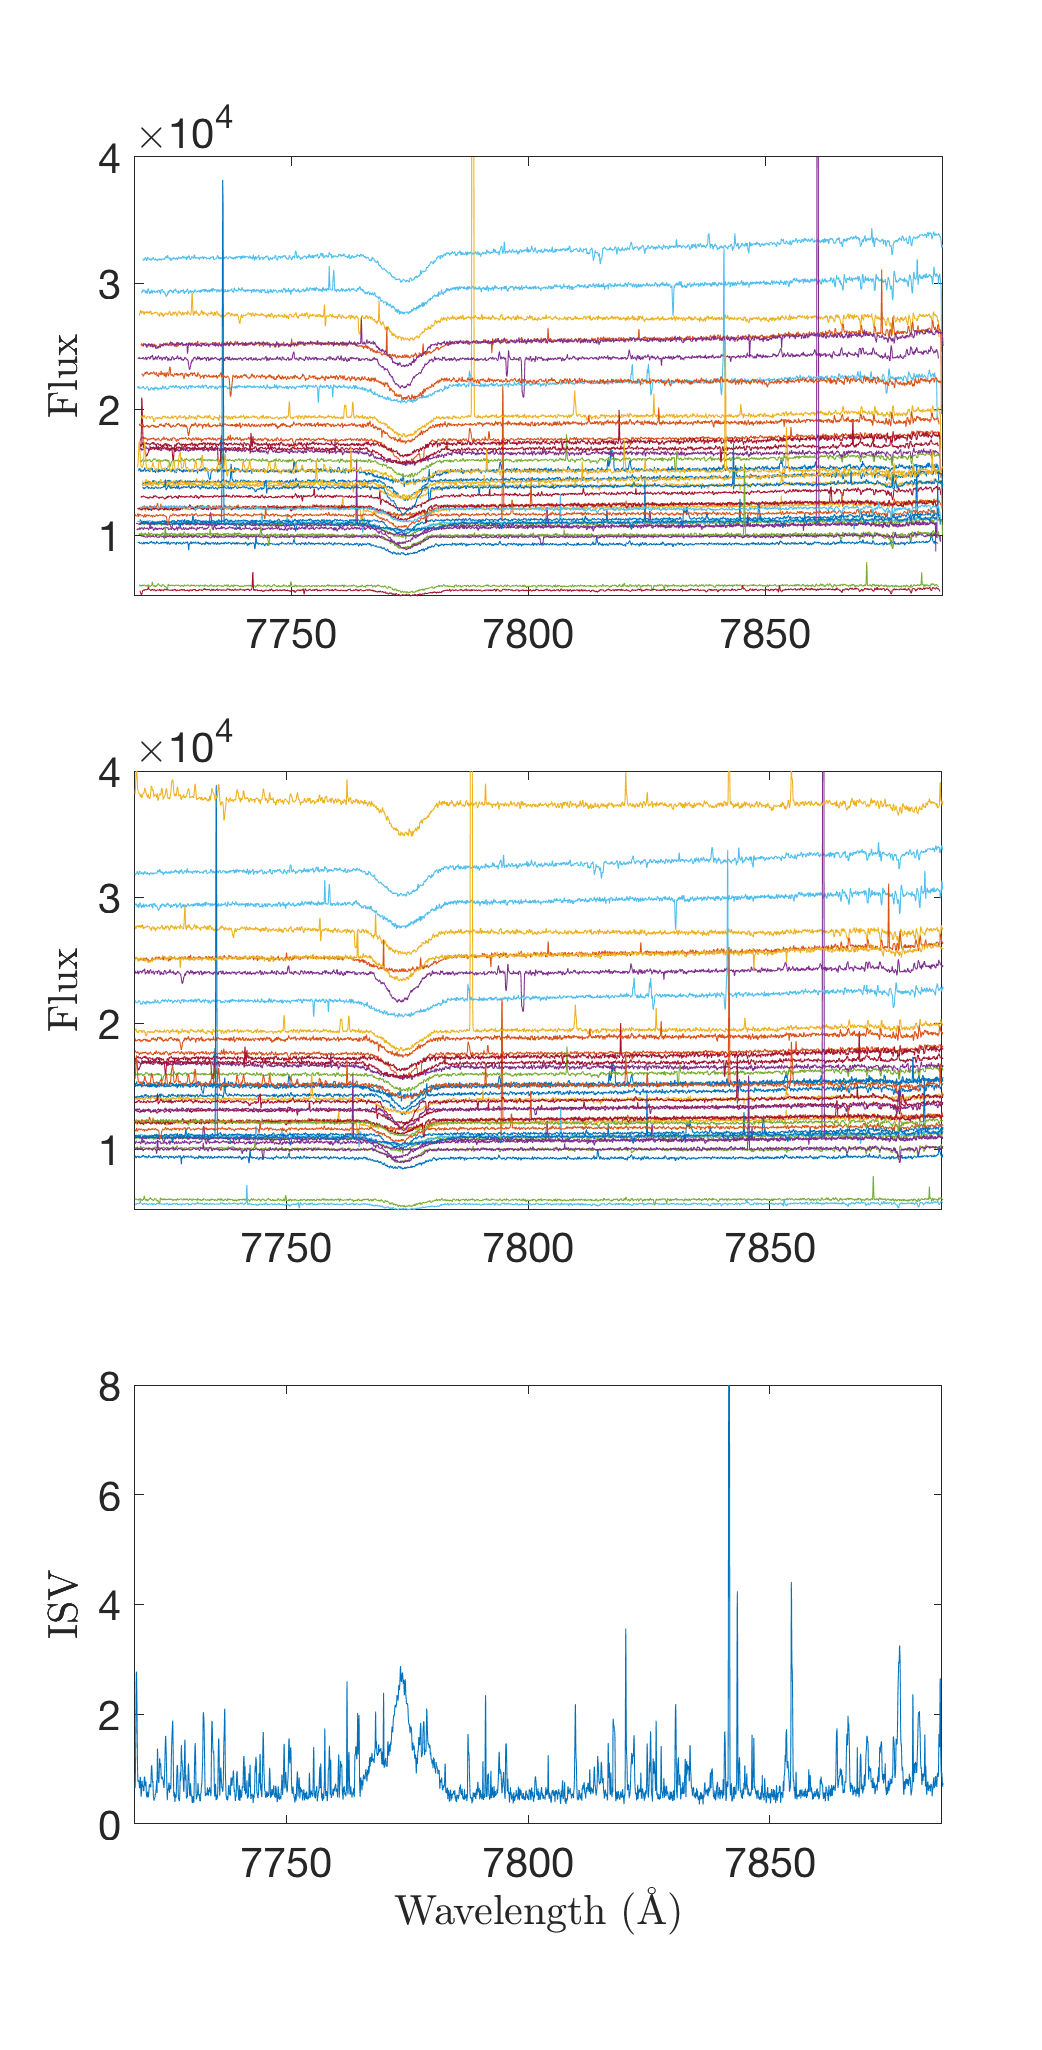
\includegraphics[width=0.6\textwidth]{GALAH_B_4.png}}\\
    \caption{(Top) GALAH spectra of 39 B-dwarfs. (Middle) The spectra once aligned onto the same wavelength scale. (Bottom) The ISV spectrum produced from the aligned spectra.}
    \label{figGALAHbstar2}
\end{figure}

The list of sky emission lines observed and measured by UVES \citep{1992Dekker} was compared to the spectra and the resulting ISV. The blue, green, and red cameras were unaffected, as any emission lines were weak and did not produce noticeable ISV lines. The infrared camera, however, did contain 13 emission lines of sufficient strength to produce some variation in the resulting ISV. Their wavelengths are marked in Figure\,\ref{figCamera4emission} with red dashed lines over an example M-dwarf spectrum and K-dwarf spectrum. As with the sky emission lines in the HARPS data, all wavelength points within two HERMES resolution elements on either side of the emission line were removed from the GALAH spectra to ensure total removal.\\

\begin{figure}
    \centering
    \captionsetup{width=.8\textwidth}
    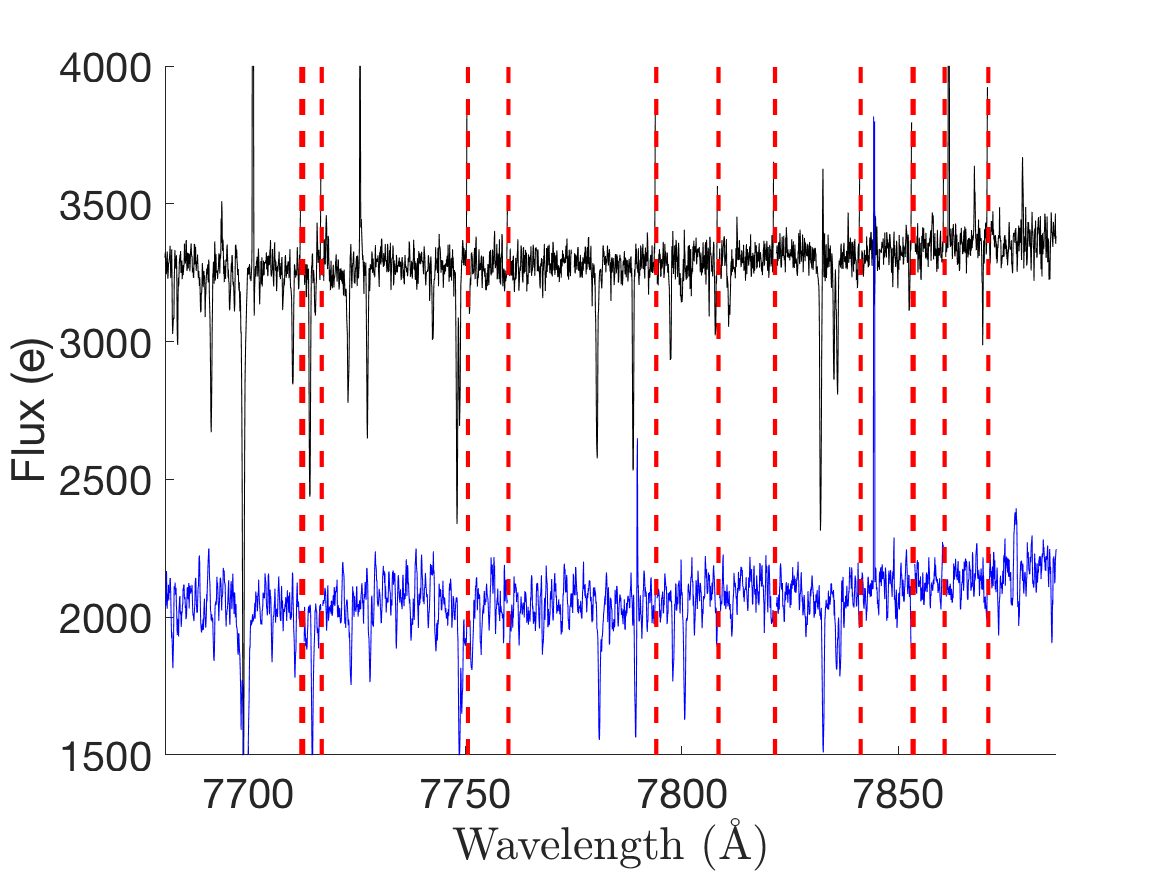
\includegraphics[width=0.8\textwidth]{GALAHskyemission.png}
    \caption{Example K-dwarf (in black) and M-dwarf (in blue) spectra for the infrared camera. The red vertical dashed lines mark the wavelengths at which strong sky emission lines are known to occur.}
    \label{figCamera4emission}
\end{figure}

\section{Equivalent width}
\label{secGALAHew}
Because the strength of an ISV line ($A_{ISV}$) was developed as an analogue to equivalent width, we expect there to be a relationship between $A_{ISV}$ and the scatter in equivalent width of the corresponding spectral line, $\sigma_{EW}$, across all observations that produced the ISV spectrum. To evaluate this relationship, the equivalent width of each spectral line corresponding to a significant ISV spectral line was measured for each observation using Equation\,\ref{eqGALAHew}. The equivalent width scatter $\sigma_{EW}$ was calculated as the standard deviation of all equivalent widths for a particular line. For a spectral line consisting of $m$ pixels, the flux across the spectral line is $I$, while the continuum level across the spectral line, $C$, is determined by clipping the entire spectrum by 3$\sigma$ and then fitting a 6th order polynomial to the clipped data.\\

While a spectroscopic signal-to-noise cut was applied to both the HARPS and GALAH samples to remove poor quality spectra, the cut had to be less stringent for HARPS as there were fewer observations per star and a harder cut would exclude a significant proportion of the spectra. As a result, the spectral lines that were identified by ISV analysis in the HARPS data are generally weaker relative to the noise, and measuring their equivalent width accurately was difficult. This is less of an obstacle for the GALAH data, for which the signal-to-noise tends to be higher (HARPS: S/N\,$\geq$\,5 per pixel in order 40, GALAH: S/N\,$\geq$\,20 per pixel in all cameras).\\

\begin{equation}
    E(\lambda) = \sum\limits_{i=1}^m \left( 1-\frac{I(\lambda)}{C(\lambda)} \right)
    \label{eqGALAHew}
\end{equation}

\section{The GALAH line list}
\label{secGALAHlinelist}
Stellar abundances are a main scientific focus of the GALAH survey. The public DR3 catalogue contains multiple physical parameters, including abundance measurements of 30 elements, for each star. To facilitate these measurements, a list of 866 lines commonly found in the spectra of Solar-type stars, spanning the GALAH wavelength range, is used. The list includes oscillator strengths and excitation potentials for each line. The list is based on the {\em Gaia}-ESO line list \citep{2015Heiter}, but with updated parameters (see Section 3.3 of \citealt{2021Buder} for details).\\

As indicated previously, the GALAH line list is an acceptable but not ideal resource for this work. The lines in the list are those found frequently in Solar-type stars. Late K-dwarfs, and especially M-dwarfs, will have different stellar structures, and therefore different spectra. Not every line found in this list is expected to be seen in the spectrum of a cooler star, and some of the lines seen in cool stars will be absent from this list. Due to the prevalence of broad molecular absorption features in the spectra of cool stars (especially M-dwarfs), a comprehensive line list specifically for cool stars is difficult to produce.\\

While Chapter\,\ref{chapISV} focused on detecting as many variable lines as possible in HARPS M-dwarf spectra, this study investigates how variability might impact abundance measurements taken from the lines in the spectra. Out of the full GALAH line list, there is a subsample of 75 lines (in 30 elements) from which GALAH determines abundances. With a few exceptions, those 75 lines are the ones used for the analysis in this chapter. Lines in the spectral region of 7590-7723\hbox{\AA} were removed from the list, since that spectroscopic region is heavily affected by telluric absorption and was clipped out (see Section\,\ref{secGALAHnonstellar}). The H$\beta$ (4861.35\hbox{\AA}) and H$\alpha$ (6562.81\hbox{\AA}) lines are not used for abundance determination by GALAH. However, they were included in the ISV line list as they are strong lines, known to vary, and helpful for ISV analysis. The ISV line list contains 73 lines, and the details are given in Table\,\ref{tabGALAHlinefinal}.\\

\begin{table}[]
    \centering
    \begin{tabular}{|l|c||l|c|}
    \hline
    Element & $\lambda$ (\AA) & Element & $\lambda$ (\AA) \\
    \hline
La\textsc{ii} & 4716.44 &   Ti\textsc{ii} & 4874.01 \\
Ti\textsc{ii} & 4719.51 & Y\textsc{ii} & 4883.68 \\ 
Sm\textsc{ii} & 4719.84 &   Y\textsc{ii} & 5662.92 \\ 
Zn\textsc{i} & 4722.15 &  Zr\textsc{i} & 5680.90 \\   
Zr\textsc{i} & 4739.48 &   Ti\textsc{i} & 5689.46 \\  
La\textsc{ii} & 4748.73 &   Ru\textsc{i} & 5699.06 \\ 
Ru\textsc{i} & 4757.85 &  Cu\textsc{i} & 5700.23 \\
Ti\textsc{i} & 4758.12 & Mg\textsc{i} & 5711.09 \\ 
Ti\textsc{i} & 4759.14 & Ti\textsc{i} & 5716.45 \\  
Ti\textsc{ii} & 4764.52 & Ti\textsc{i} & 5720.43 \\
Zr\textsc{i} & 4772.31 &   Y\textsc{ii} & 5728.89 \\ 
Ce\textsc{ii} & 4773.94 &  Ti\textsc{i} & 5739.47 \\ 
Ti\textsc{i} & 4778.25 & Nd\textsc{ii} & 5740.86 \\ 
Co\textsc{i} & 4781.43 & Nd\textsc{ii} & 5770.49 \\ 
Ti\textsc{i} & 4781.71 & Cu\textsc{i} & 5782.13 \\ 
V\textsc{i} & 4784.47 &  La\textsc{ii} & 5805.77 \\  
Sm\textsc{ii} & 4791.58 &   Nd\textsc{ii} & 5811.57 \\  
V\textsc{i} & 4796.91 &   Eu\textsc{ii} & 5818.74 \\
Ti\textsc{i} & 4797.98 & Nd\textsc{ii} & 5842.37 \\ 
Ti\textsc{ii} & 4798.53 & Ni\textsc{i} & 5846.99 \\
Ti\textsc{i} & 4801.95 & Ti\textsc{i} & 5866.45 \\
La\textsc{ii} & 4804.03 & Co\textsc{i} & 6490.34 \\
Zr\textsc{i} & 4805.87 &   Sr\textsc{i} & 6550.24 \\ 
Zn\textsc{i} & 4810.53 &   Co\textsc{i} & 6551.45 \\
Nd\textsc{ii} & 4811.34 &  H\textsc{i} & 6562.81 \\   
Y\textsc{i} & 4819.64 &  Ni\textsc{i} & 6586.31 \\
Ti\textsc{i} & 4820.41 & C\textsc{i} & 6587.61 \\   
Zr\textsc{i} & 4828.04 &   Ti\textsc{i} & 6599.10 \\
V\textsc{i} & 4831.65 &  Co\textsc{i} & 6632.44 \\
Sm\textsc{ii} & 4836.66 &   Eu\textsc{ii} & 6645.10 \\
Sm\textsc{ii} & 4847.76 &   Co\textsc{i} & 6678.81 \\
Ti\textsc{ii} & 4849.17 & Li\textsc{i} & 6707.91 \\
Sm\textsc{ii} & 4854.35 & Ti\textsc{i} & 6716.67 \\ 
Y\textsc{ii} & 4854.86 &  Rb\textsc{i} & 7800.26 \\ 
H\textsc{i} & 4861.35 &    Co\textsc{i} & 7838.13 \\
Ti\textsc{i} & 4865.78 & Ti\textsc{i} & 7852.68 \\ 
Ru\textsc{i} & 4869.15 &  & \\
\hline
    \end{tabular}
    \caption{The edited GALAH line list used for this work.}
    \label{tabGALAHlinefinal}
\end{table}

\section{Results}
\label{secGALAHresults}
\begin{figure}
	\captionsetup{width=.8\textwidth}
	\hspace{-2cm}
	\subfloat[Blue]{\label{figGALAH_ISV_camera1}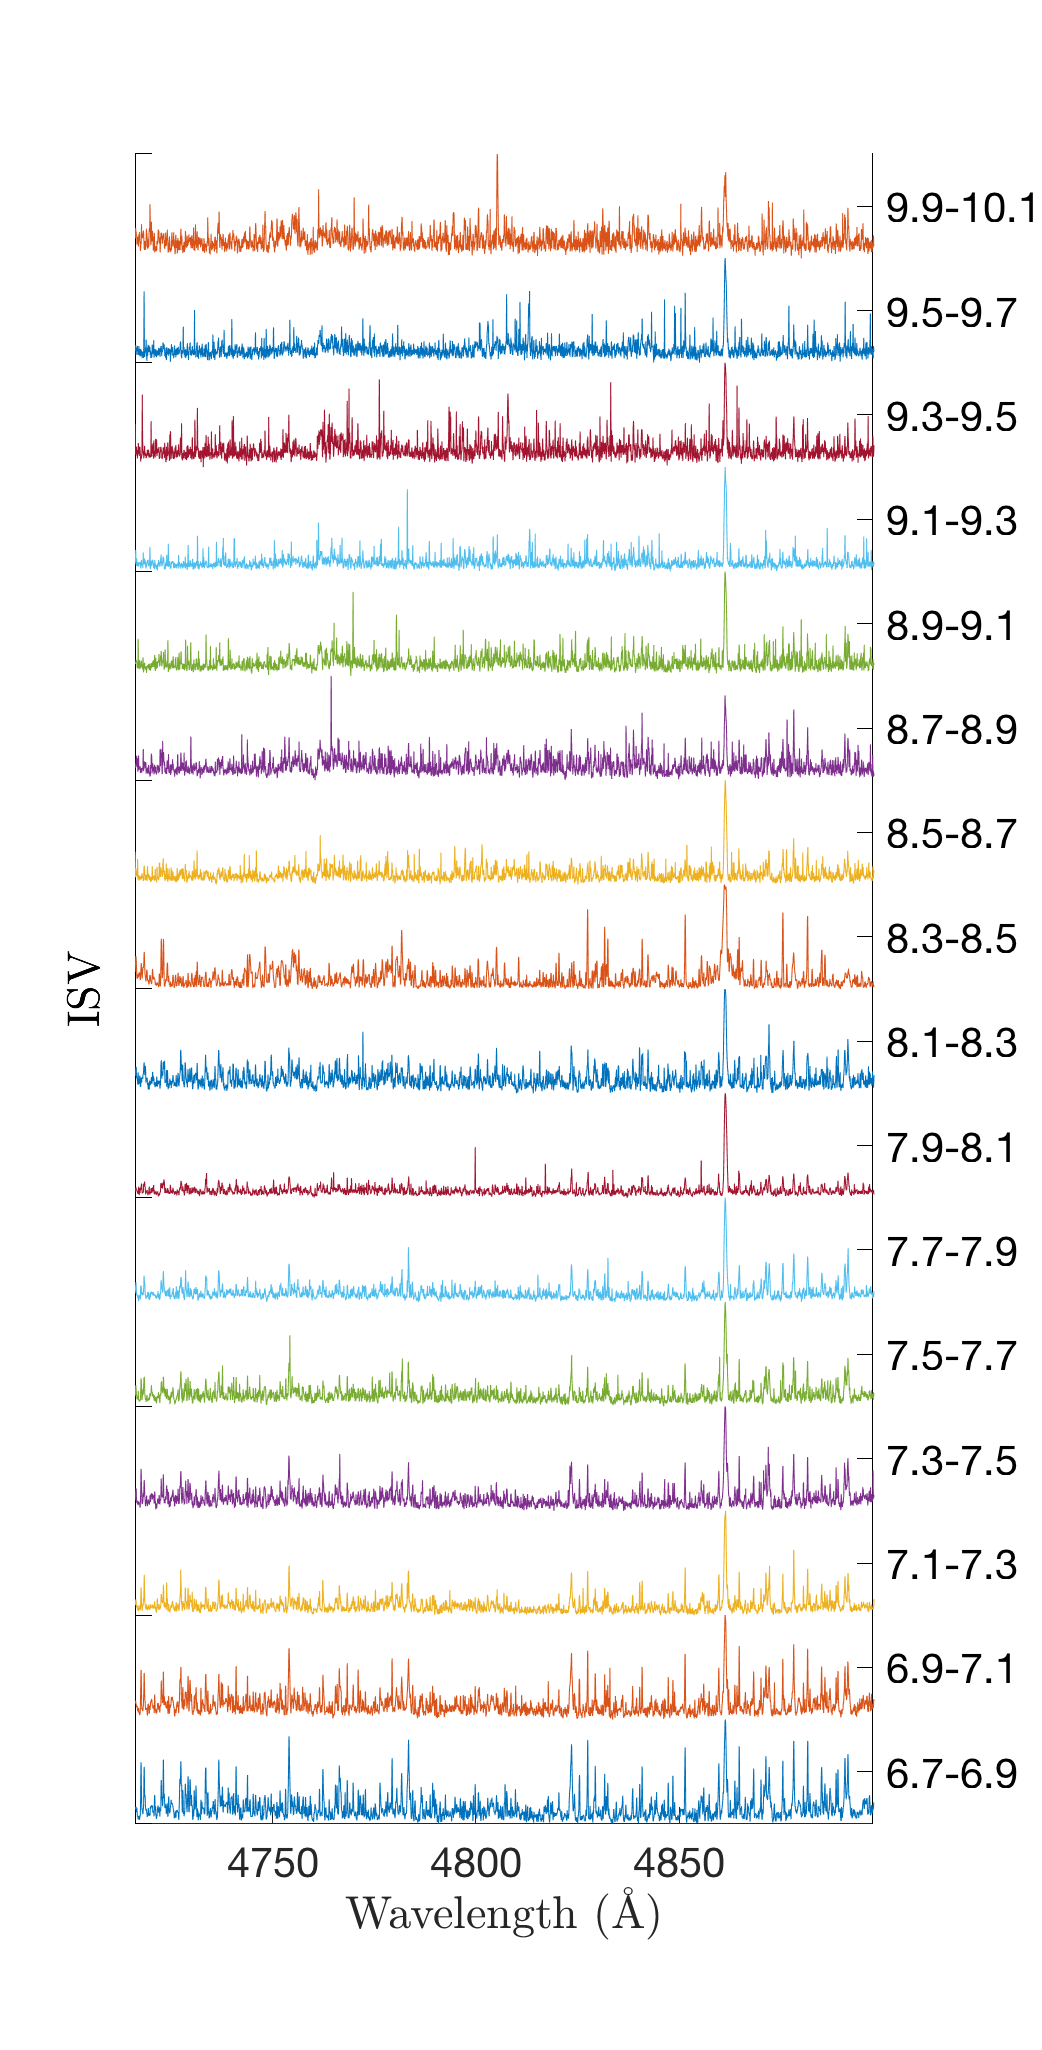
\includegraphics[width=0.6\textwidth]{GALAH_ISV_camera_1.png}}
    \subfloat[Green]{\label{figGALAH_ISV_camera2}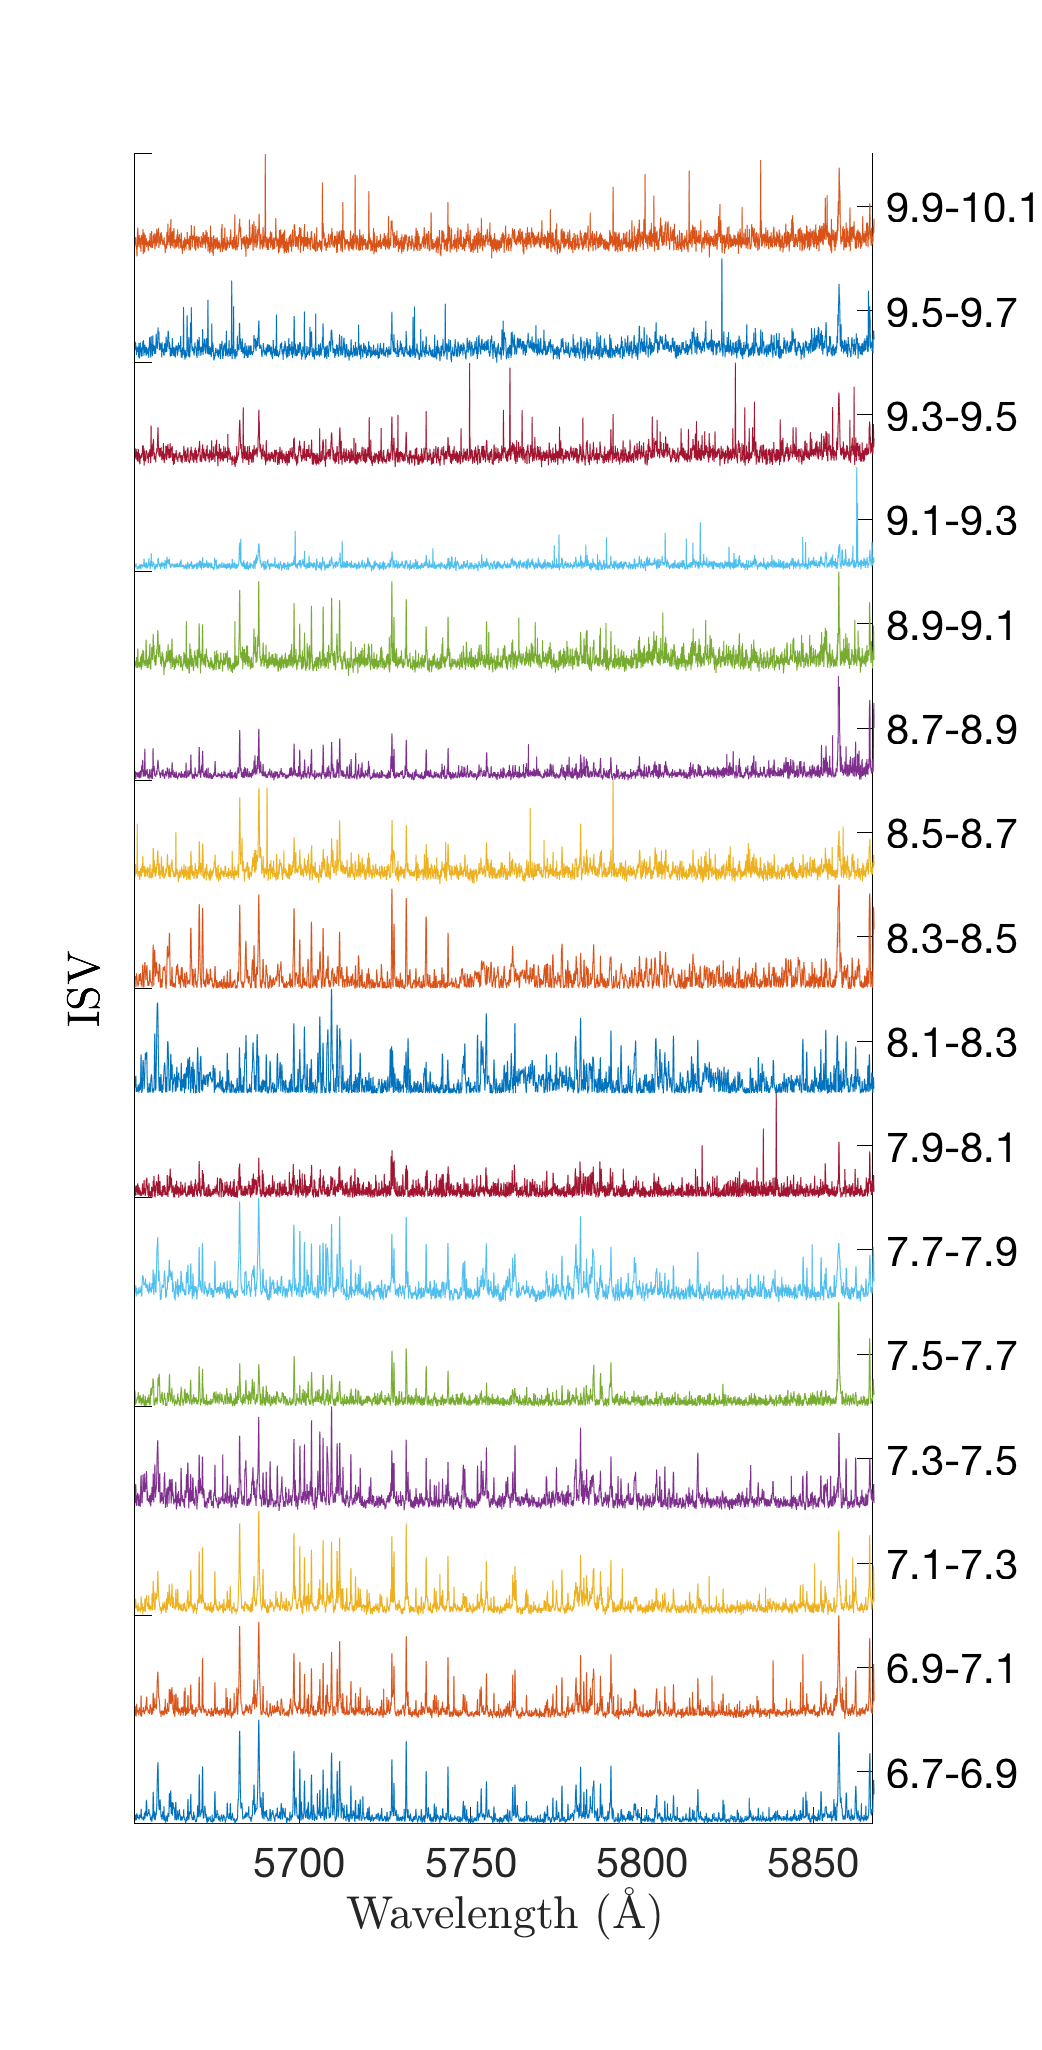
\includegraphics[width=0.6\textwidth]{GALAH_ISV_camera_2.png}}\\
    \caption{ISV plots for each absolute magnitude bin. Each spectrum has been normalised and offset in the y-axis for visual clarity, and the absolute magnitude bins range from $M_G$\,=\,6.7-6.9 at the bottom, to $M_G$\,=\,9.9-10.1 at the top.}
\end{figure}
\begin{figure}
	\captionsetup{width=.8\textwidth}
	\hspace{-2cm}
    \subfloat[Red]{\label{figGALAH_ISV_camera3}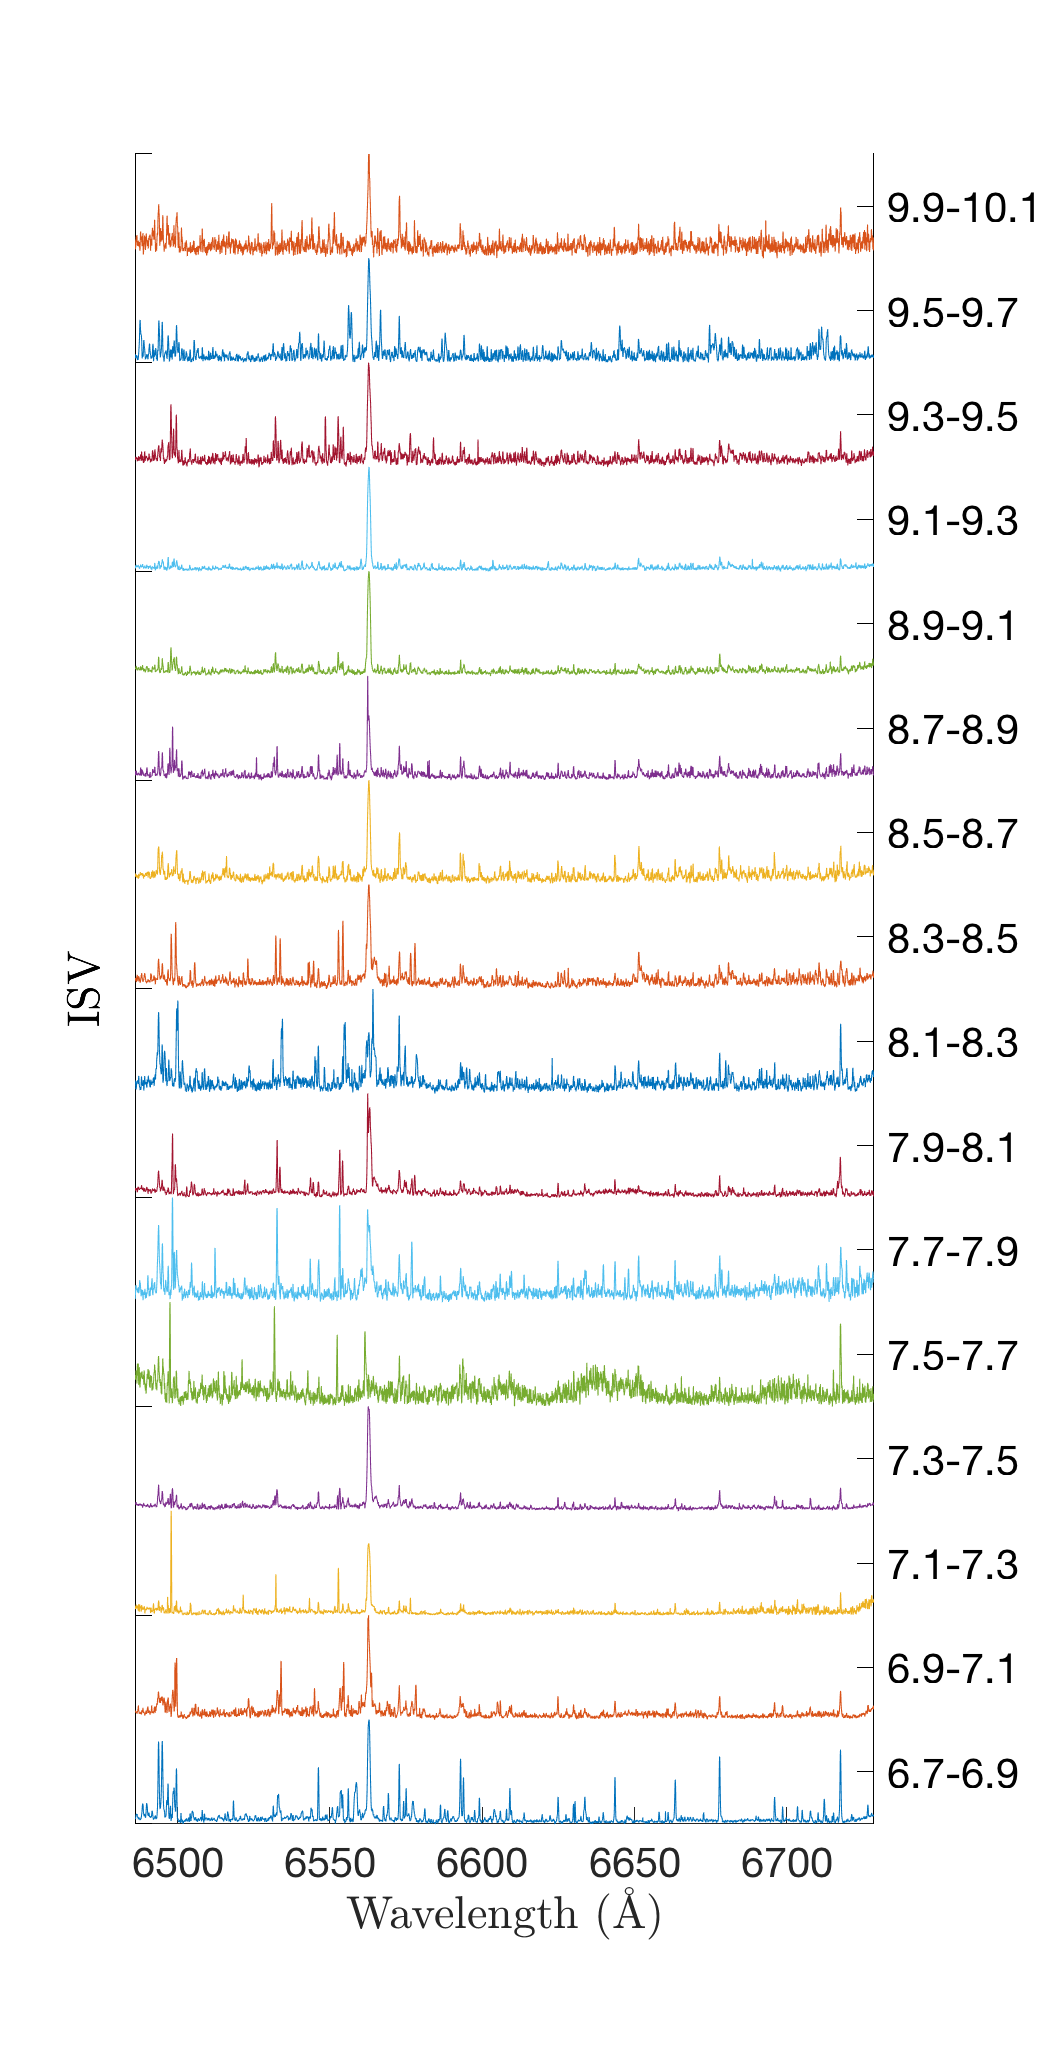
\includegraphics[width=0.6\textwidth]{GALAH_ISV_camera_3.png}}
    \subfloat[Infrared]{\label{figGALAH_ISV_camera4}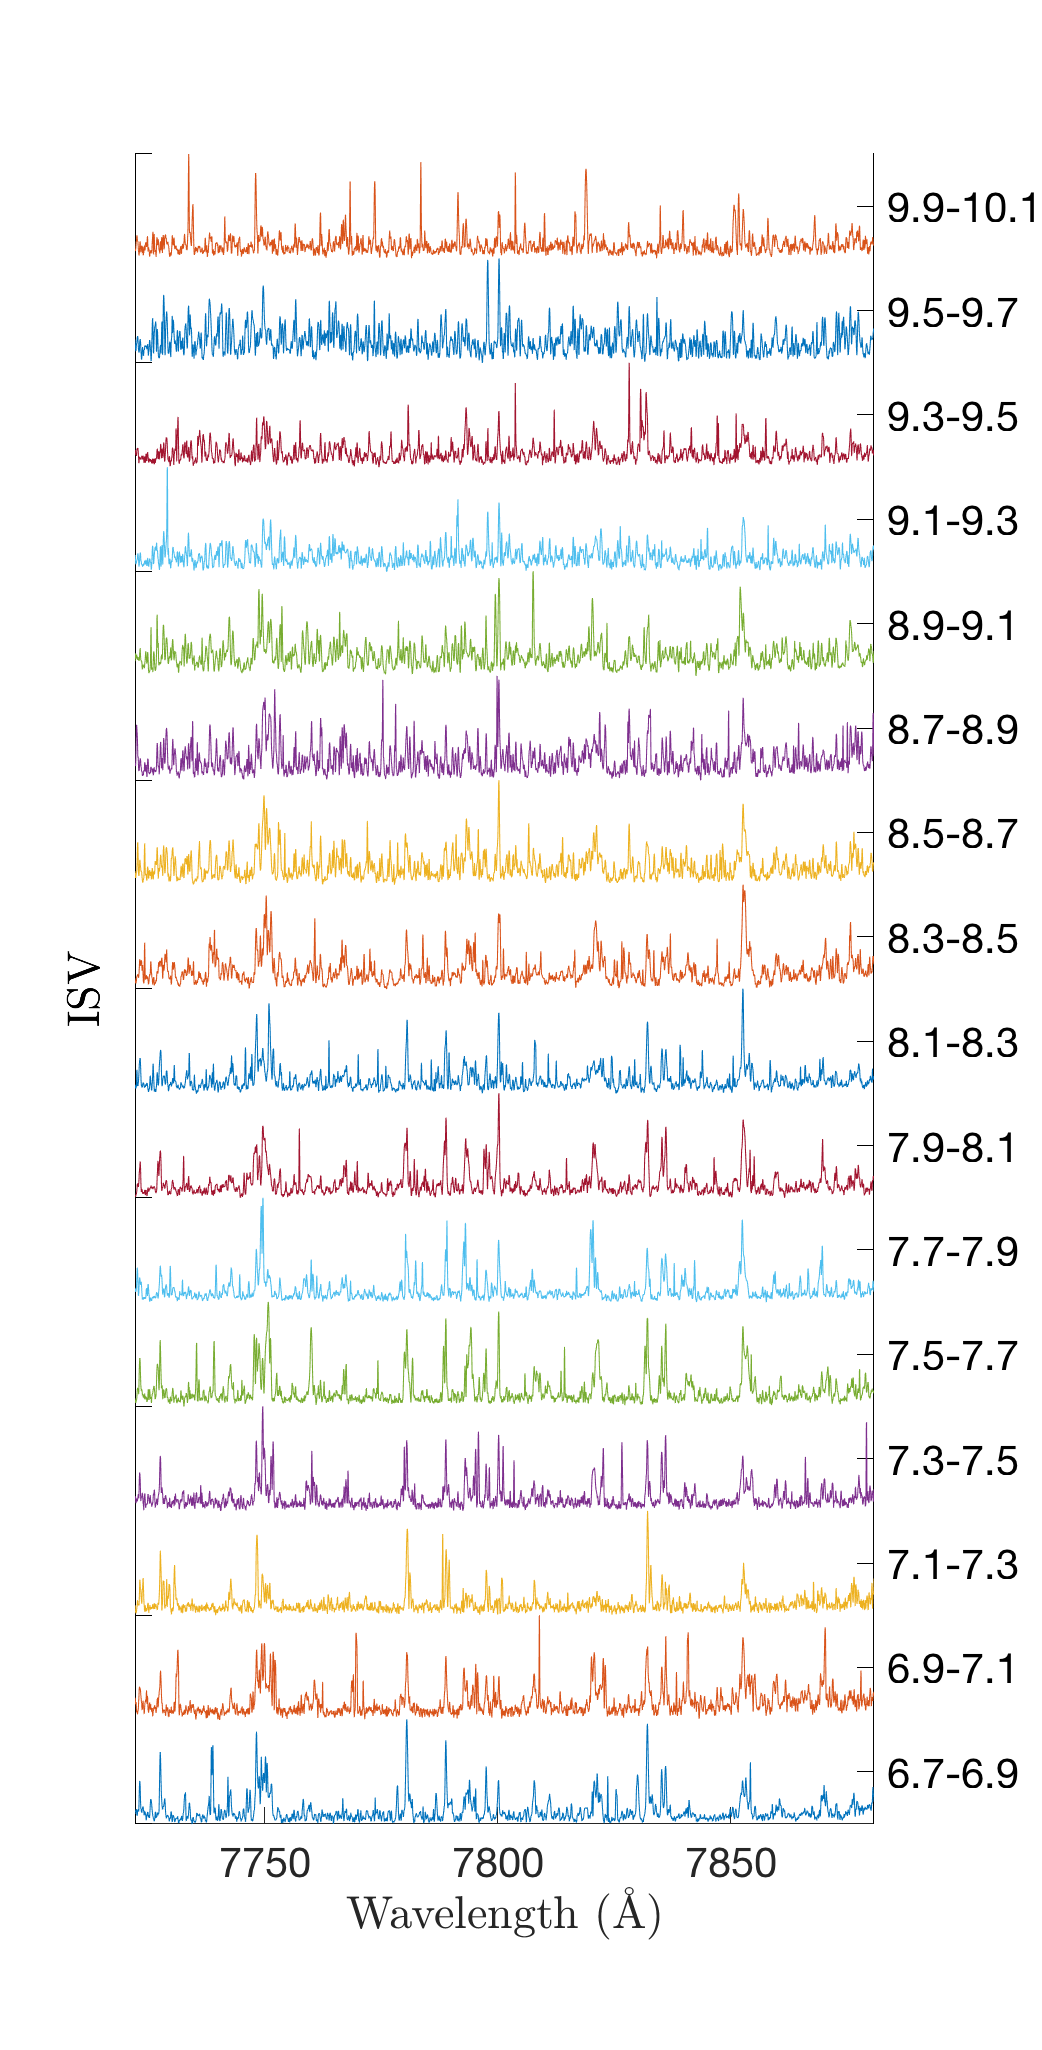
\includegraphics[width=0.6\textwidth]{GALAH_ISV_camera_4.png}}\\
    \caption{ISV plots each absolute magnitude bin. Each spectrum has been normalised and offset in the y-axis for visual clarity, and the absolute magnitude bins range from $M_G$\,=\,6.7-6.9 at the bottom, to $M_G$\,=\,9.9-10.1 at the top.}
\end{figure}

The selected GALAH spectra were prepared as per Section\,\ref{secGALAHalteration}, with problematic wavelengths masked out as per Section\,\ref{secGALAHnonstellar}. ISV spectra for each camera and each absolute magnitude bin were produced and are presented in Figures\,\ref{figGALAH_ISV_camera1}-\ref{figGALAH_ISV_camera4}. These figures have been normalised and offset to aid visibility. It is clear that there are ISV lines common to most, if not all, absolute magnitude bins, and that their strength varies with absolute magnitude. The ISV spectral lines were identified, and the $A_{ISV}$ was measured. The equivalent widths of the spectral lines corresponding to the ISV spectral lines were measured. Additionally, the median S-index for H$\alpha$ was measured for each bin.\\
 
\subsection{ISV line properties}
\begin{figure}
	\captionsetup{width=.8\textwidth}
    \subfloat[M-dwarf transition energies]{\label{figGALAH_trans_M}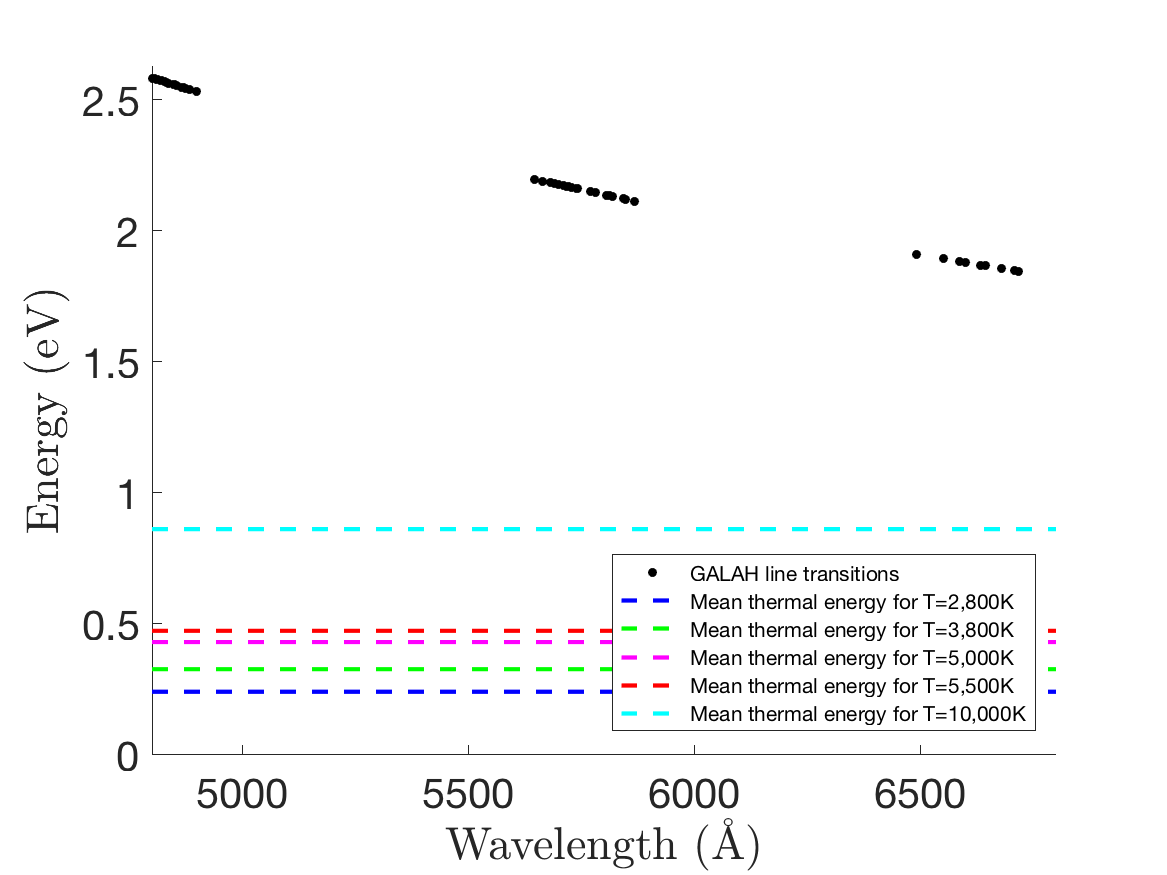
\includegraphics[width=0.5\textwidth]{GALAH_MD_trans.png}}
    \subfloat[Solar transition energies]{\label{figGALAH_trans_G}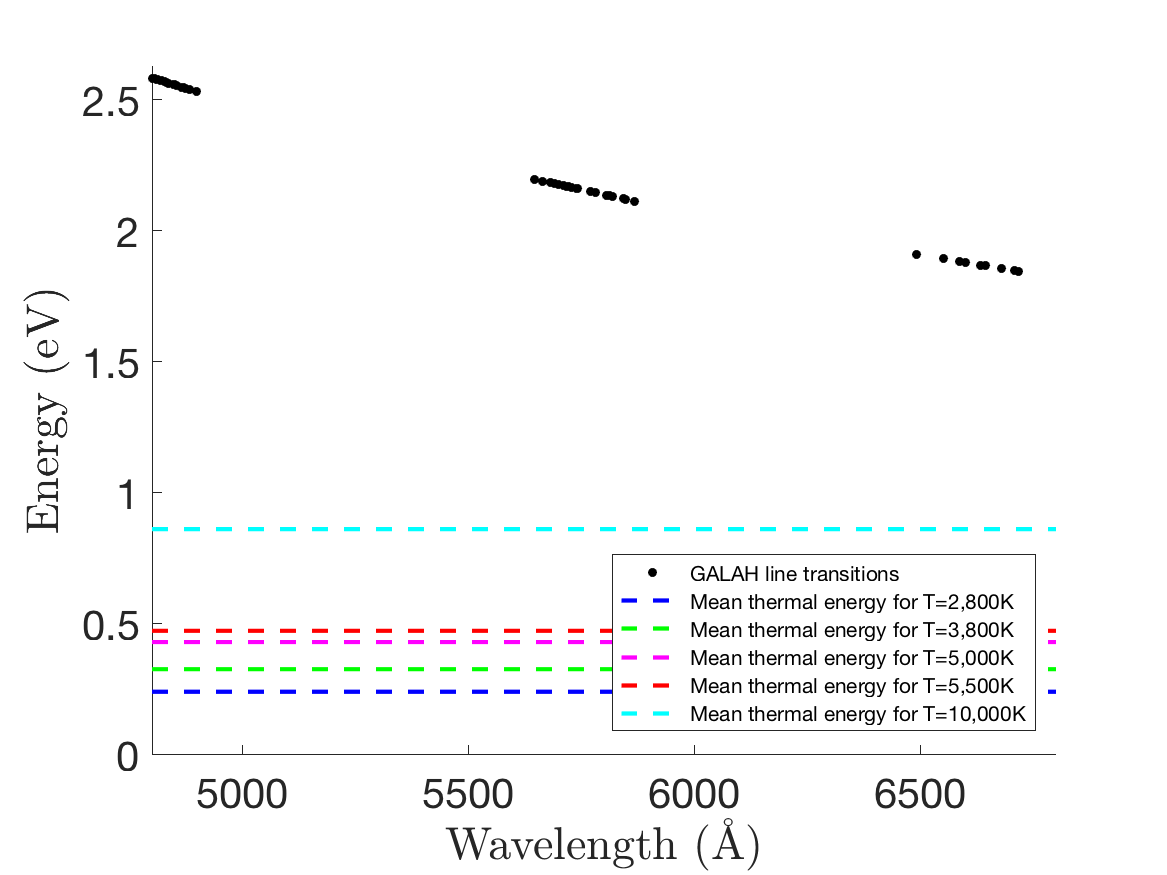
\includegraphics[width=0.5\textwidth]{GALAH_GD_trans.png}}\\
    \subfloat[M-dwarf ionisation energies]{\label{figGALAH_ion_M}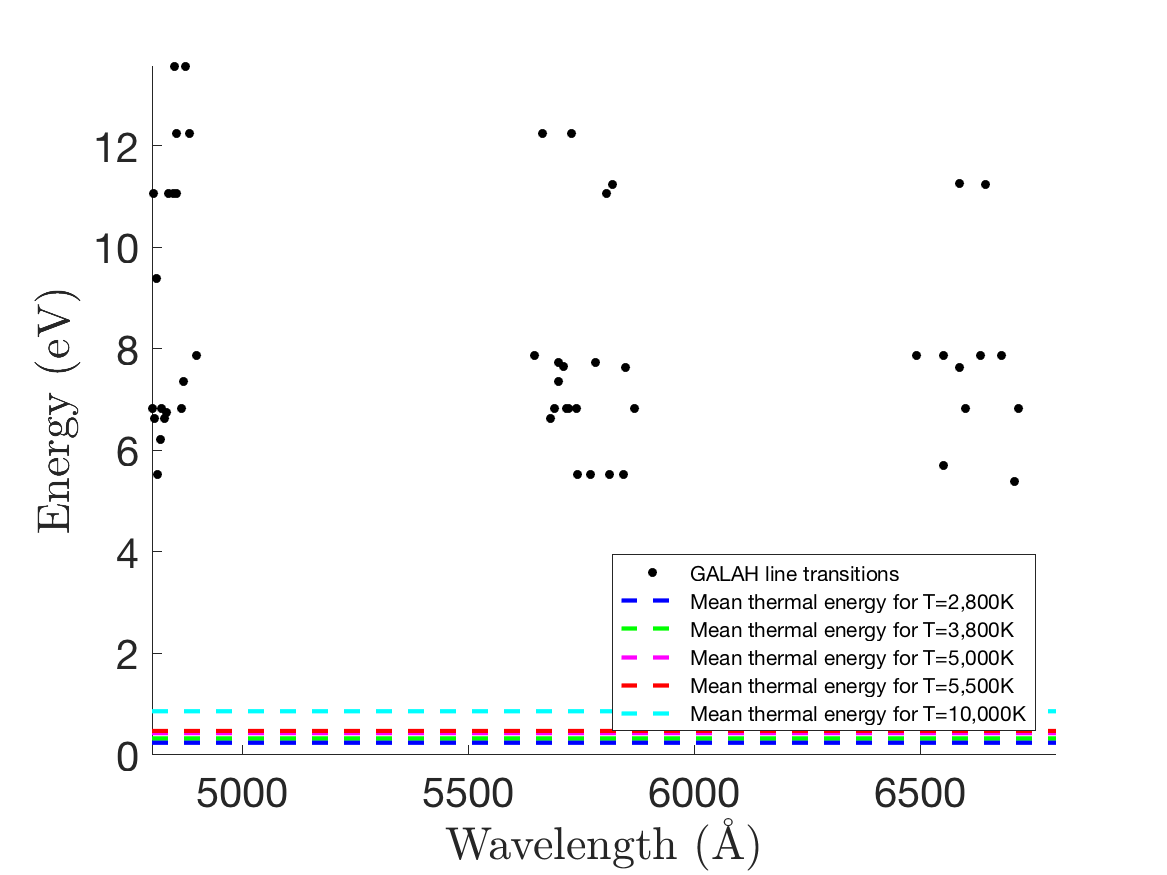
\includegraphics[width=0.5\textwidth]{GALAH_MD_ion.png}}
    \subfloat[Solar ionisation energies]{\label{figGALAH_ion_G}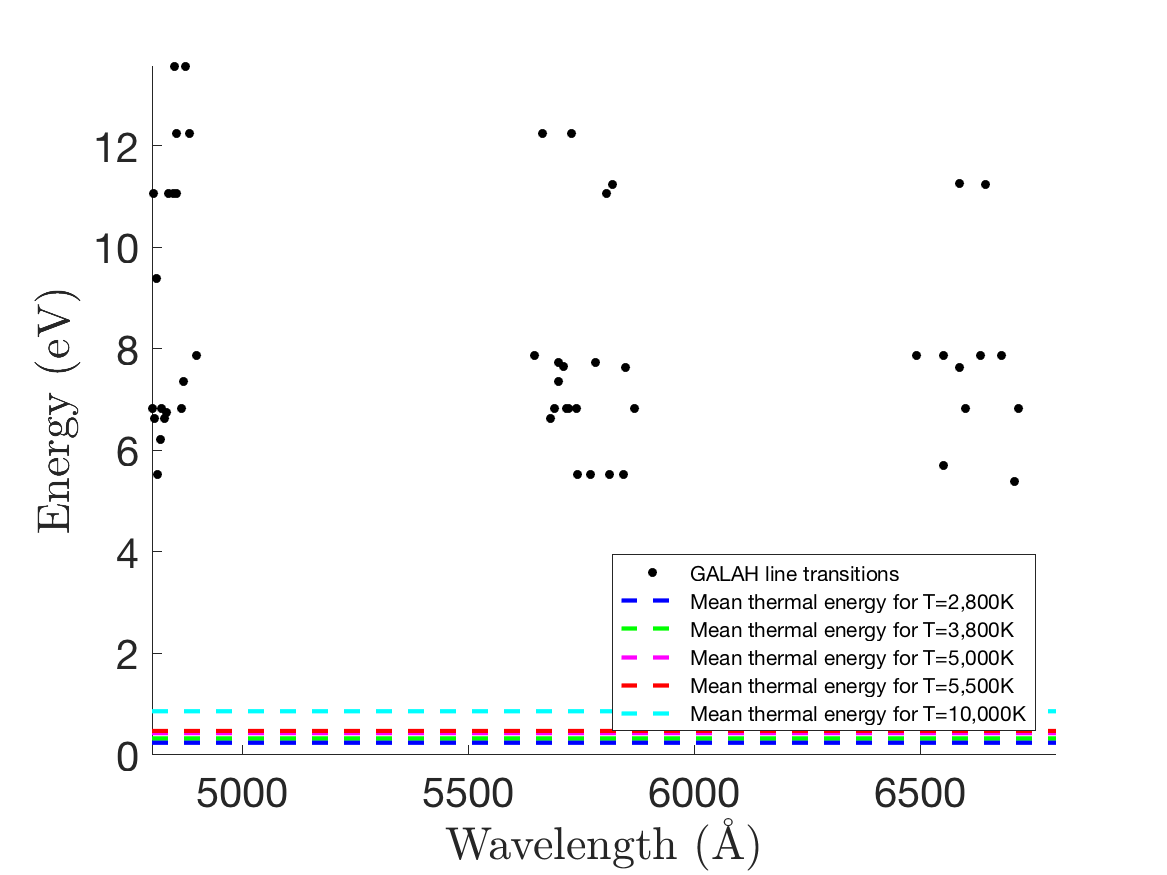
\includegraphics[width=0.5\textwidth]{GALAH_GD_ion.png}}\\
    \caption{Plots showing the transition energy (top) and ionisation potential (bottom) for the 73 lines in our edited GALAH line list. The red, green, blue, magenta, and cyan dashed lines represent the mean thermal energy at T\,=\,2,800, 3,800, 5,000, 5,500, and 10,000K.}
\end{figure}

As with the HARPS data, interpreting the ISV spectra requires a physical understanding of the layer of the star at which the lines being studied are produced. The transition and ionisation energies for these lines are needed to do this. Plots of transition and ionisation energy vs wavelength were produced using the M-dwarf photosphere and chromosphere temperatures used in Section\,\ref{secResults}.\\

As K-dwarfs are hotter than M-dwarfs, a second set of photosphere and chromosphere temperatures were required. Given the lack of a suitable set of atmospheric temperature data for K-dwarfs in the literature, an upper limit can be obtained by considering the properties of a Sun-like star. Any transitions found to be produced in the same region of the Sun and an M-dwarf would also be found at the same region in a K-dwarf, since its temperature is intermediate. Temperatures of the photosphere and chromosphere for the Sun were taken from \citet{2017Linsky}, specifically, the lower bound of the photosphere (7,000\,K), the upper photosphere/lower chromosphere boundary (5,000\,K), the lower/upper chromosphere boundary (3,800\,K), and the transition region (6,300\,K). The solar upper chromosphere/corona boundary is at 1.2x10$^{6}$\,K, corresponding to a mean thermal energy of 103.4\,eV. Figures\,\ref{figGALAH_trans_M}-\ref{figGALAH_ion_G} present the thermal energies for each layer of the star, and the transition and ionisation energies for each line in the ISV line list. As with the HARPS M-dwarfs, all spectral lines found in the ISV line list require transition energies well above the transition region, and require ionisation energy far in excess of that provided by both the photosphere and chromosphere. As is typical for spectral lines affected by stellar activity, the absorption component of the line is formed in the photosphere and distorted by various surface processes. Similar to the strong ISV lines in the HARPS sample, in the GALAH sample the upper chromosphere has sufficient energy to drive further variability through emission in the spectral lines that exhibit ISV.\\

\subsection{Variable lines in GALAH spectra}
\label{secGALAHlines}
In Chapter\,\ref{chapISV} there was a focus on which ISV spectral lines were present in multiple M-dwarfs, and we required that the ISV spectral lines used for further analysis were found in at least ten stars. For this chapter, the focus is on lines found to vary in ensembles of stars in narrow absolute magnitude bins. An ISV spectral line needed to be identified in at least 5 of the 16 bins to be considered for further analysis. Of the 137 spectral lines found to be varying in the ISV spectra, 10 of them varied in $\geq$5 of the ISV absolute magnitude binned spectra, and the details of these lines are presented in Table\,\ref{tabGALAHfreqlines}. Unlike the ISV spectral lines that were frequently varying in HARPS data, these lines are spread out across the full wavelength range used, and there is no species that is more common than any other.\\

\begin{table}[]
    \centering
    \begin{tabular}{|l|c|c||l|c|c|}
    \hline
    Element & Wavelength & Frequency & Element & Wavelength & Frequency \\
     & ($\lambda$) & (\#) &   & ($\lambda$) & (\#) \\
     \hline
Ti\textsc{i} & 4781.71 & 7 & Cu\textsc{i} & 5782.13 & 13 \\ 
V\textsc{i} & 4831.65 & 9 &   Ti\textsc{i} & 5866.45 & 14 \\
H\textsc{i} & 4861.35 & 16 &    H\textsc{i} & 6562.81 & 16 \\   
Cu\textsc{i} & 5700.23 & 8 &  Rb\textsc{i} & 7800.26 & 16 \\ 
Mg\textsc{i} & 5711.09 & 6 &   Ti\textsc{i} & 7852.68 & 9 \\  
\hline
    \end{tabular}
    \caption{Spectral lines found to vary in at least 5 of the absolute magnitude-binned ISV spectra. Frequency is the number of ISV spectra the line was found to be varying in.}
    \label{tabGALAHfreqlines}
\end{table}

The $A_{ISV}$ magnitude and measurement error were calculated for each line in Table\,\ref{tabGALAHfreqlines}, and this information is presented as a series of figures (\ref{figGALAH_line_evo_1}-\ref{figGALAH_line_evo_10}). These show the ISV line strength $A_{ISV}$ and its uncertainty for each absolute magnitude bin in blue, and the percentage measurement uncertainty (\%$A_{ISV}$) in red.\\

\begin{figure}
    \hspace{-2cm}
	\captionsetup{width=.8\textwidth}
	\subfloat[Ti\,\textsc{i} (4781.71\hbox{\AA})]{\label{figGALAH_line_evo_1}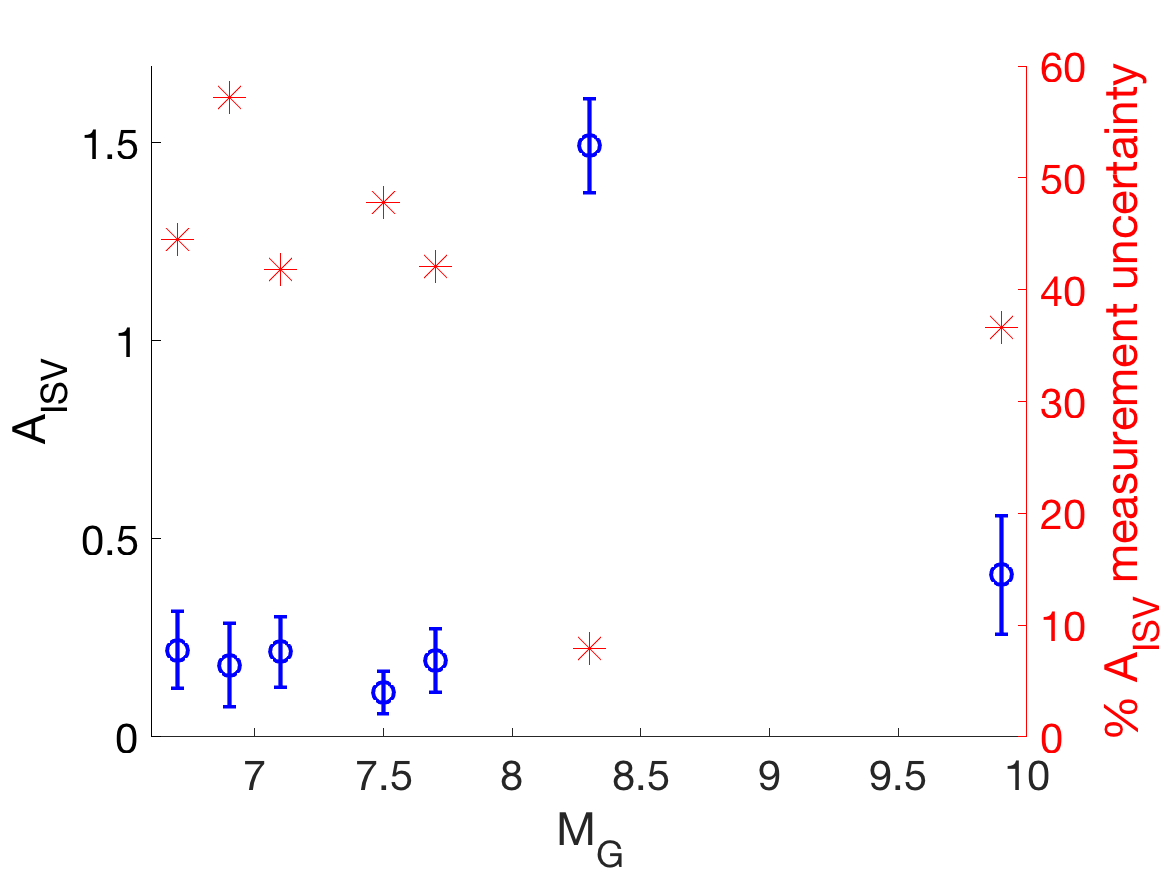
\includegraphics[width=0.6\textwidth]{GALAH_Line_Plots/GALAH_ISV_line_4781_7106_Ti1.png}}
	\subfloat[V\,\textsc{i} (4831.65\hbox{\AA})]{\label{figGALAH_line_evo_2}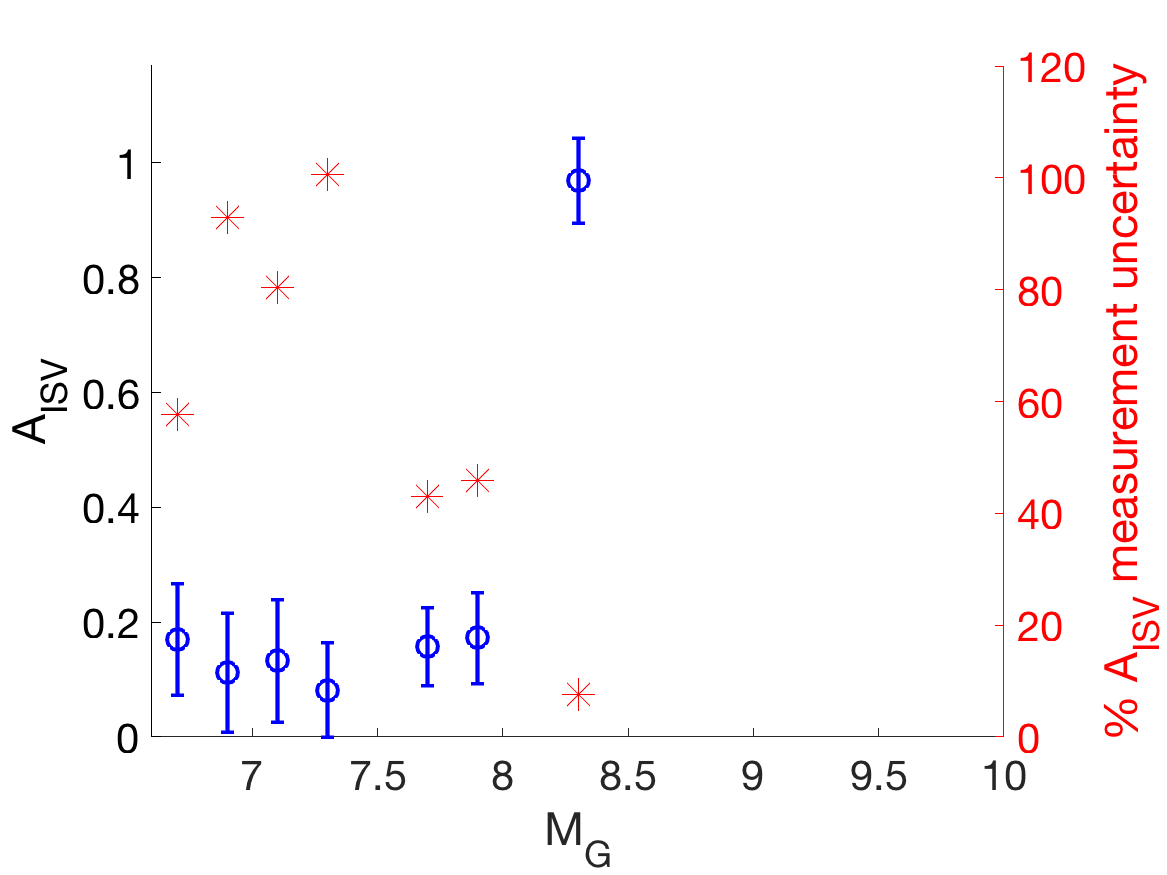
\includegraphics[width=0.6\textwidth]{GALAH_Line_Plots/GALAH_ISV_line_4831_6457_V1.png}}
    \caption{Plots of the $A_{ISV}$ magnitude, with uncertainties (in blue), and \% uncertainty (in red) for specific lines found to be varying in the absolute magnitude binned ISV spectra.}
    \label{figGALAH_evo_1}
\end{figure}

\begin{figure}
    \hspace{-2cm}
	\captionsetup{width=.8\textwidth}
	\subfloat[H\,\textsc{i} (4861.35\hbox{\AA})]{\label{figGALAH_line_evo_3}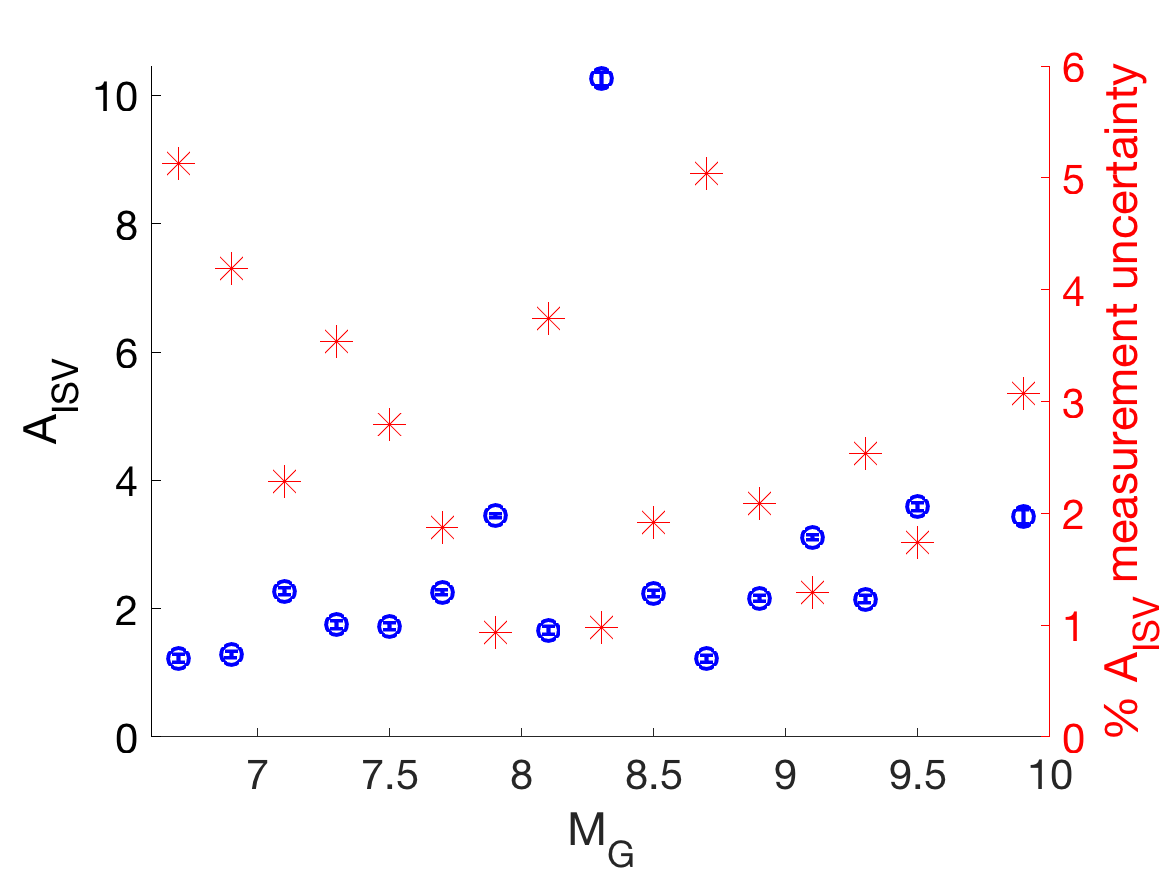
\includegraphics[width=0.6\textwidth]{GALAH_Line_Plots/GALAH_ISV_line_4861_35_H1.png}}
	\subfloat[Cu\,\textsc{i} (5700.23\hbox{\AA})]{\label{figGALAH_line_evo_4}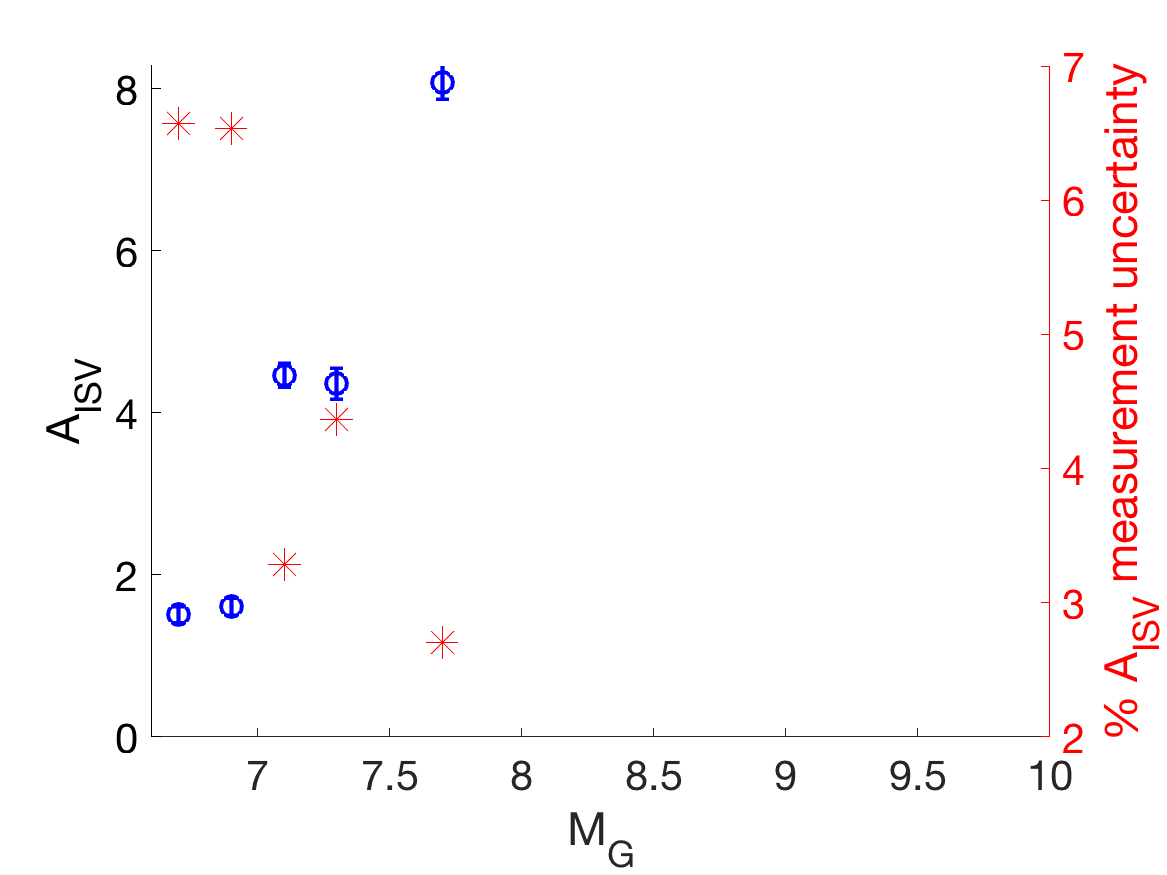
\includegraphics[width=0.6\textwidth]{GALAH_Line_Plots/GALAH_ISV_line_5700_2326_Cu1.png}}
    \caption{Plots of the $A_{ISV}$ magnitude, with uncertainties (in blue), and \% uncertainty (in red) for specific lines found to be varying in the absolute magnitude binned ISV spectra.}
    \label{figGALAH_evo_2}
\end{figure}

\begin{figure}
    \hspace{-2cm}
	\captionsetup{width=.8\textwidth}
	\subfloat[Mg\,\textsc{i} (5711.09\hbox{\AA})]{\label{figGALAH_line_evo_5}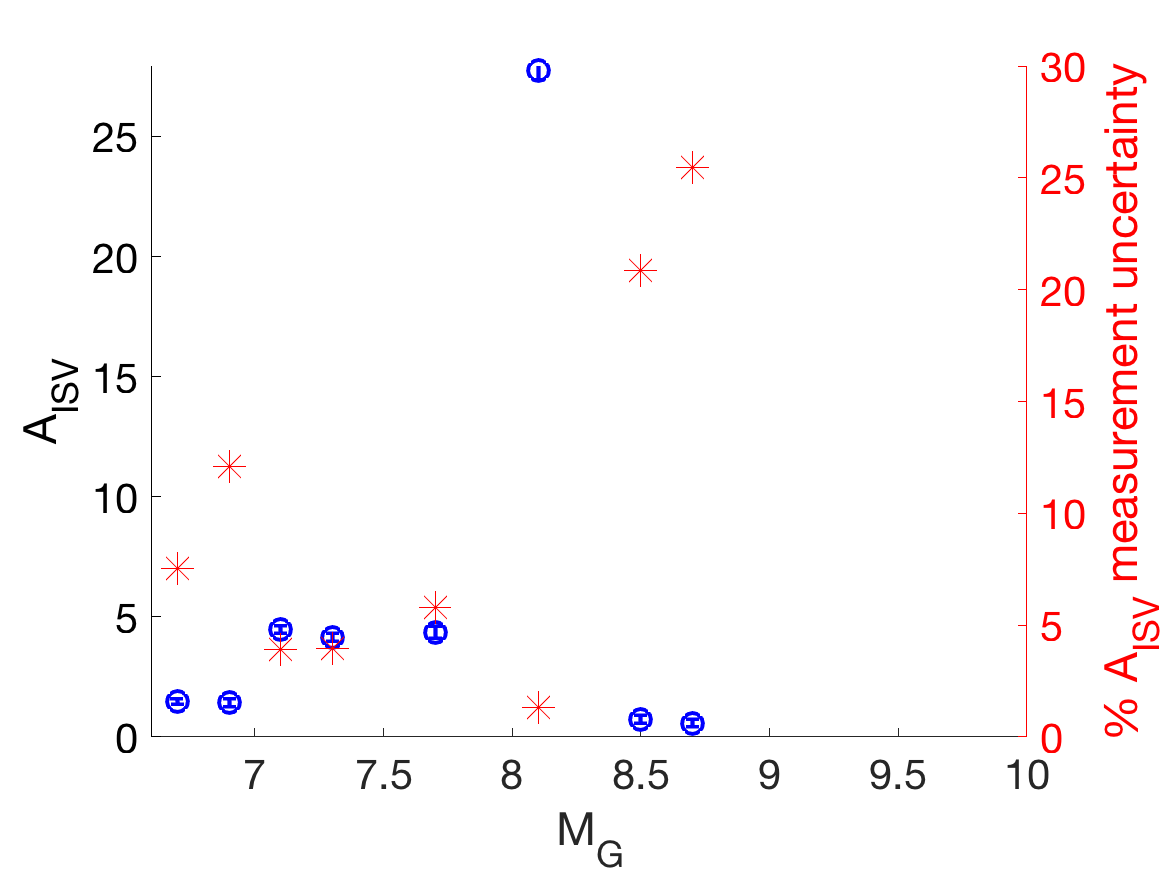
\includegraphics[width=0.6\textwidth]{GALAH_Line_Plots/GALAH_ISV_line_5711_088_Mg1.png}}
	\subfloat[Cu\,\textsc{i} (5782.13\hbox{\AA})]{\label{figGALAH_line_evo_6}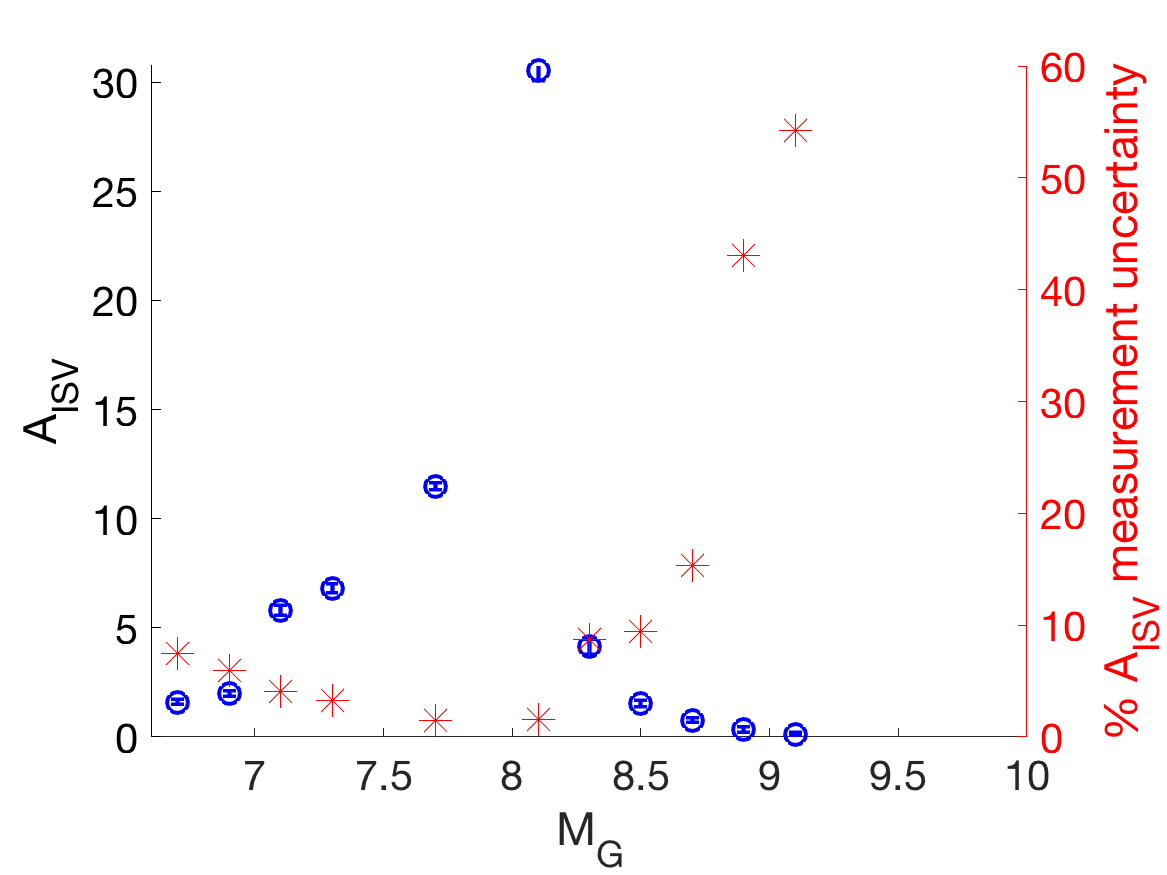
\includegraphics[width=0.6\textwidth]{GALAH_Line_Plots/GALAH_ISV_line_5782_125_Cu1.png}}
    \caption{Plots of the $A_{ISV}$ magnitude, with uncertainties (in blue), and \% uncertainty (in red) for specific lines found to be varying in the absolute magnitude binned ISV spectra.}
    \label{figGALAH_evo_3}
\end{figure}

\begin{figure}
    \hspace{-2cm}
	\captionsetup{width=.8\textwidth}
	\subfloat[Ti\,\textsc{i} (5866.45\hbox{\AA})]{\label{figGALAH_line_evo_7}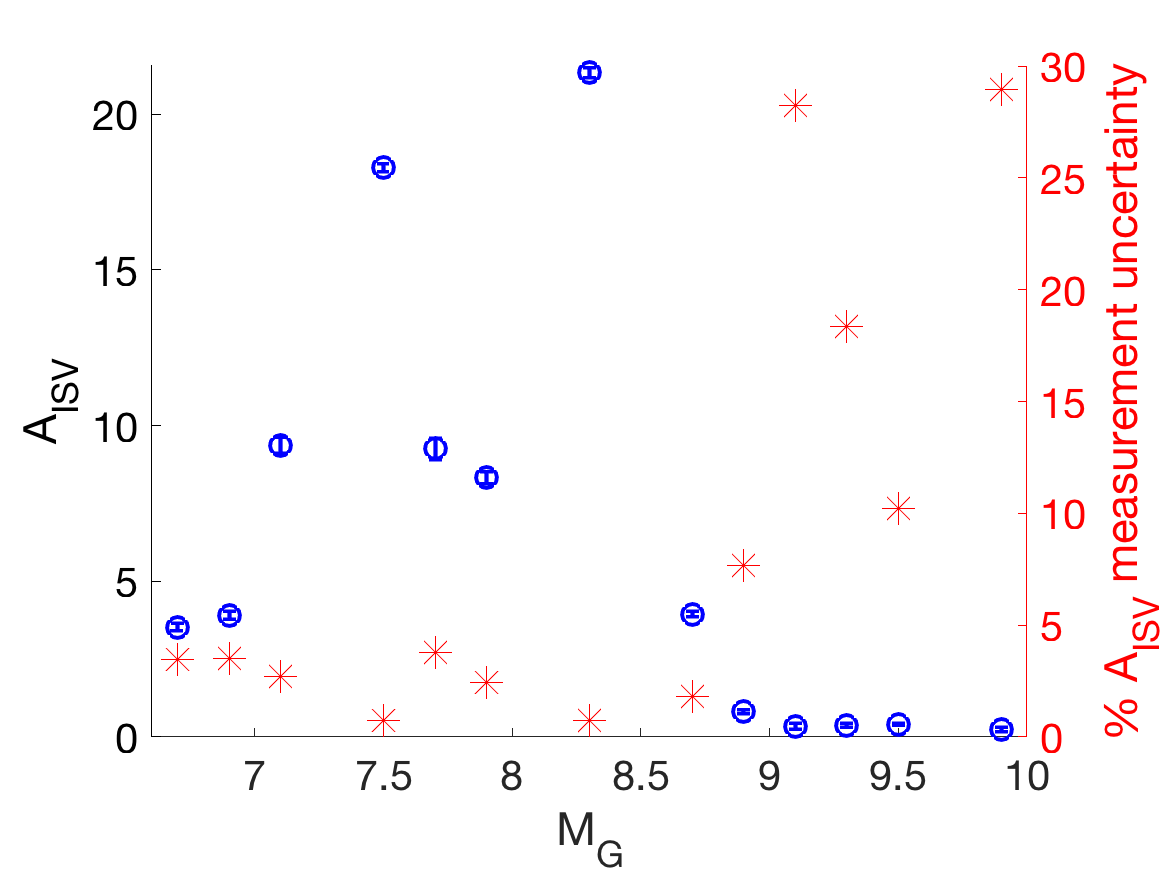
\includegraphics[width=0.6\textwidth]{GALAH_Line_Plots/GALAH_ISV_line_5866_4513_Ti1.png}}
	\subfloat[H\,\textsc{i} (6562.81\hbox{\AA})]{\label{figGALAH_line_evo_8}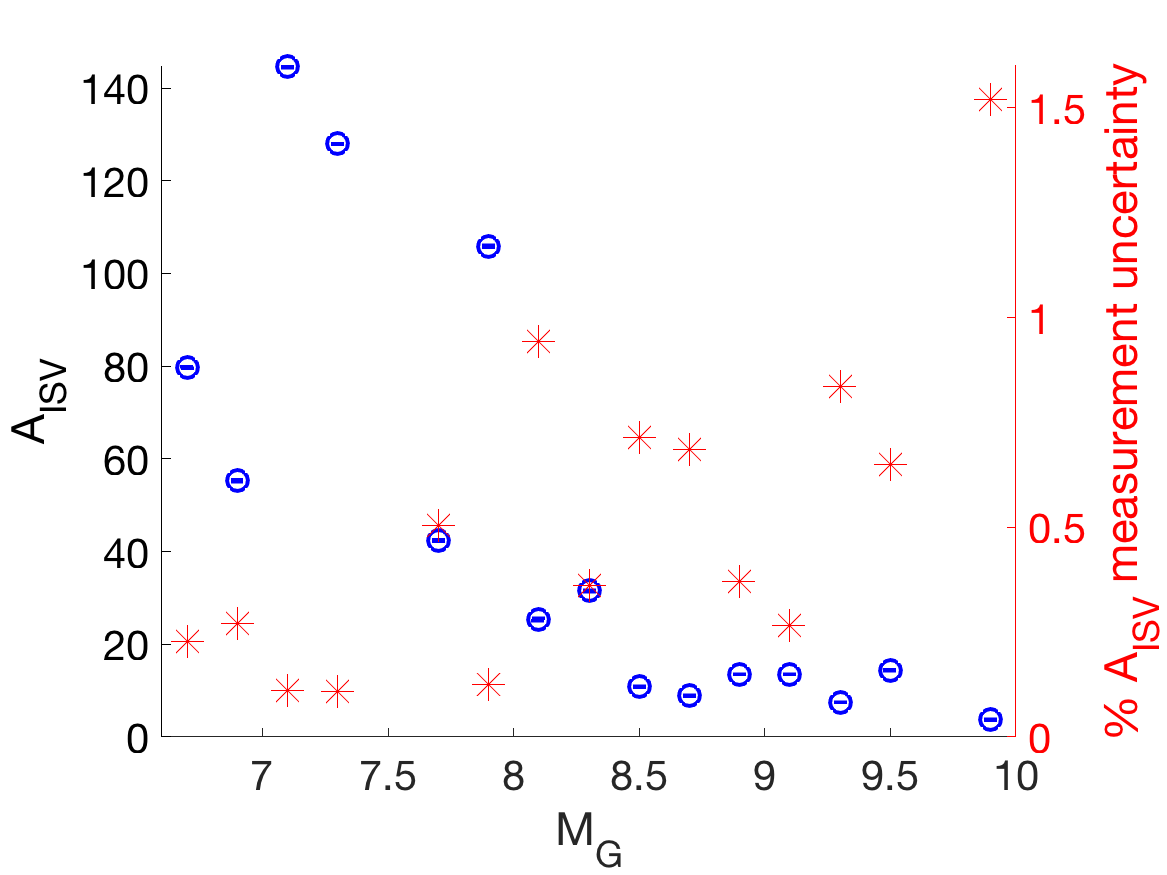
\includegraphics[width=0.6\textwidth]{GALAH_Line_Plots/GALAH_ISV_line_6562_81_H1.png}}
    \caption{Plots of the $A_{ISV}$ magnitude, with uncertainties (in blue), and \% uncertainty (in red) for specific lines found to be varying in the absolute magnitude binned ISV spectra.}
    \label{figGALAH_evo_4}
\end{figure}

\begin{figure}
    \hspace{-2cm}
	\captionsetup{width=.8\textwidth}
	\subfloat[Rb\,\textsc{i} 7800.26\hbox{\AA})]{\label{figGALAH_line_evo_9}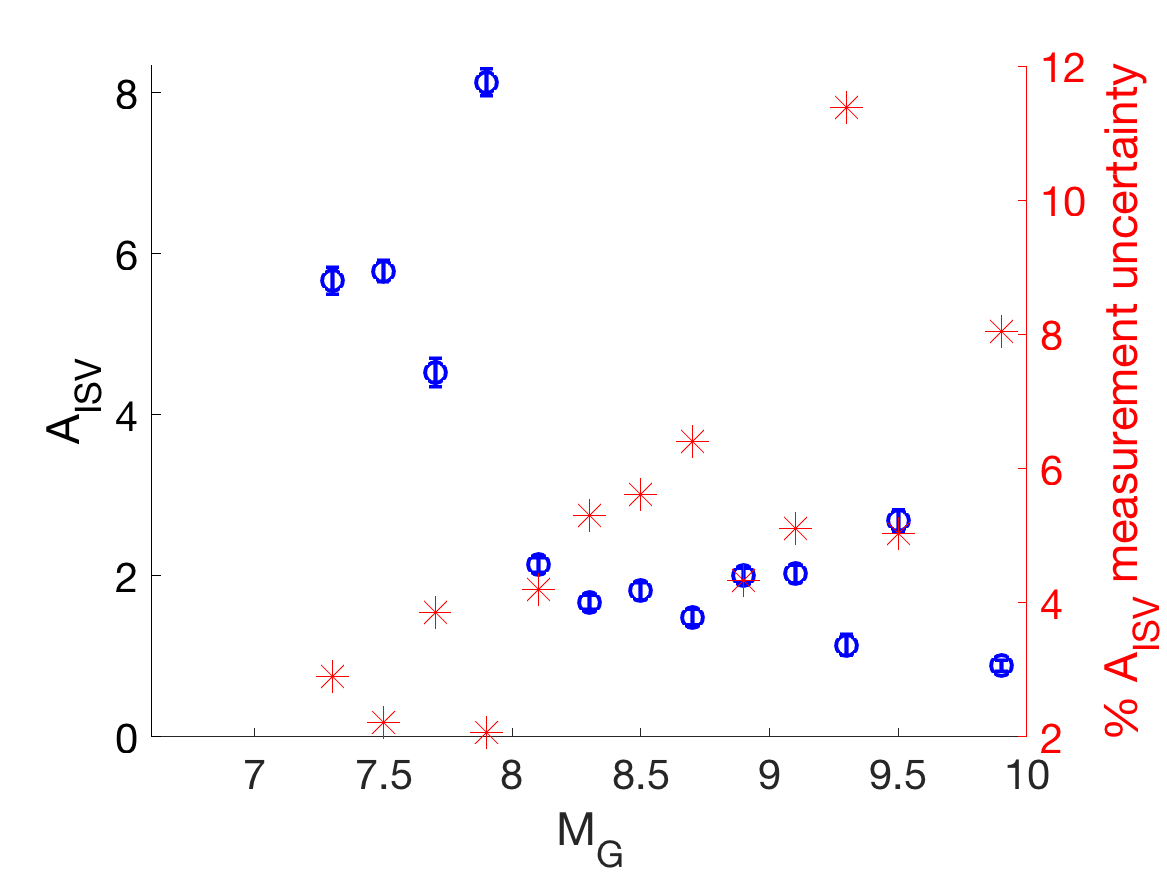
\includegraphics[width=0.6\textwidth]{GALAH_Line_Plots/GALAH_ISV_line_7800_259_Rb1.png}}
	\subfloat[Ti\,\textsc{i} (7852.68\hbox{\AA})]{\label{figGALAH_line_evo_10}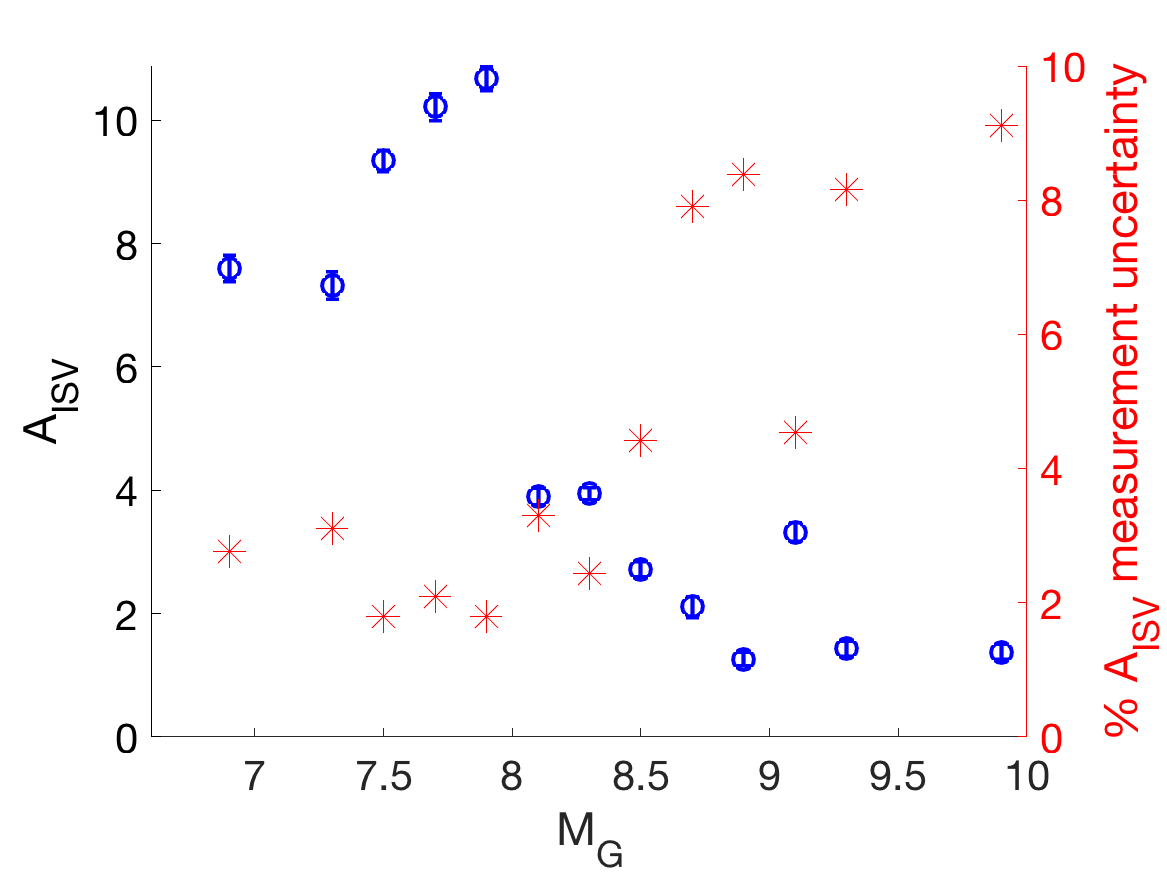
\includegraphics[width=0.6\textwidth]{GALAH_Line_Plots/GALAH_ISV_line_7852_677_Ti1.png}}
    \caption{Plots of the $A_{ISV}$ magnitude, with uncertainties (in blue), and \% uncertainty (in red) for specific lines found to be varying in the absolute magnitude binned ISV spectra.}
    \label{figGALAH_evo_5}
\end{figure}

For most of the ISV lines there is a break in behaviour between the K- and M-dwarfs. Three of the ISV lines, Ti\,\textsc{i} at 4781.71\hbox{\AA}, V\,\textsc{i} at 4831.65\hbox{\AA}, and Cu\,\textsc{i} at 5700.23\hbox{\AA}, are only detected in the K-dwarfs. Four of the lines, Ti\,\textsc{i} at 5866.45\hbox{\AA}, H\,\textsc{i} at 6562.81\hbox{\AA}, Rb\,\textsc{i} at 7800.26\hbox{\AA}, and Ti\,\textsc{i} at 7852.68\hbox{\AA}, have stronger and more variable ISV measurements for K-dwarfs than M-dwarfs. The remaining three lines, H\,\textsc{i} at 4861.35\hbox{\AA}, Mg\,\textsc{i} at 5711.09\hbox{\AA}, Cu\,\textsc{i} at 5782.13\hbox{\AA}, show strong ISV in one bin near the K-M transition but no clear trends with absolute magnitude. The size of the measurement uncertainty in $A_{ISV}$ in any given line is consistent across the magnitude bins, and so the percent uncertainty varies inversely to the strength of the line.\\

\subsection{Impact of $M_G$ on measurement uncertainty}
\label{secGALAHuncertainty}
As the sample contains a large collection of spectra across a range of stellar luminosity and spectroscopic quality, it is useful to examine the main sources of uncertainty in the $A_{ISV}$ measurement. The two main factors contributing to the measurement uncertainty are the spectroscopic signal-to-noise, and the number of observations used to create the ISV spectrum.\\

\begin{figure}
    \centering
    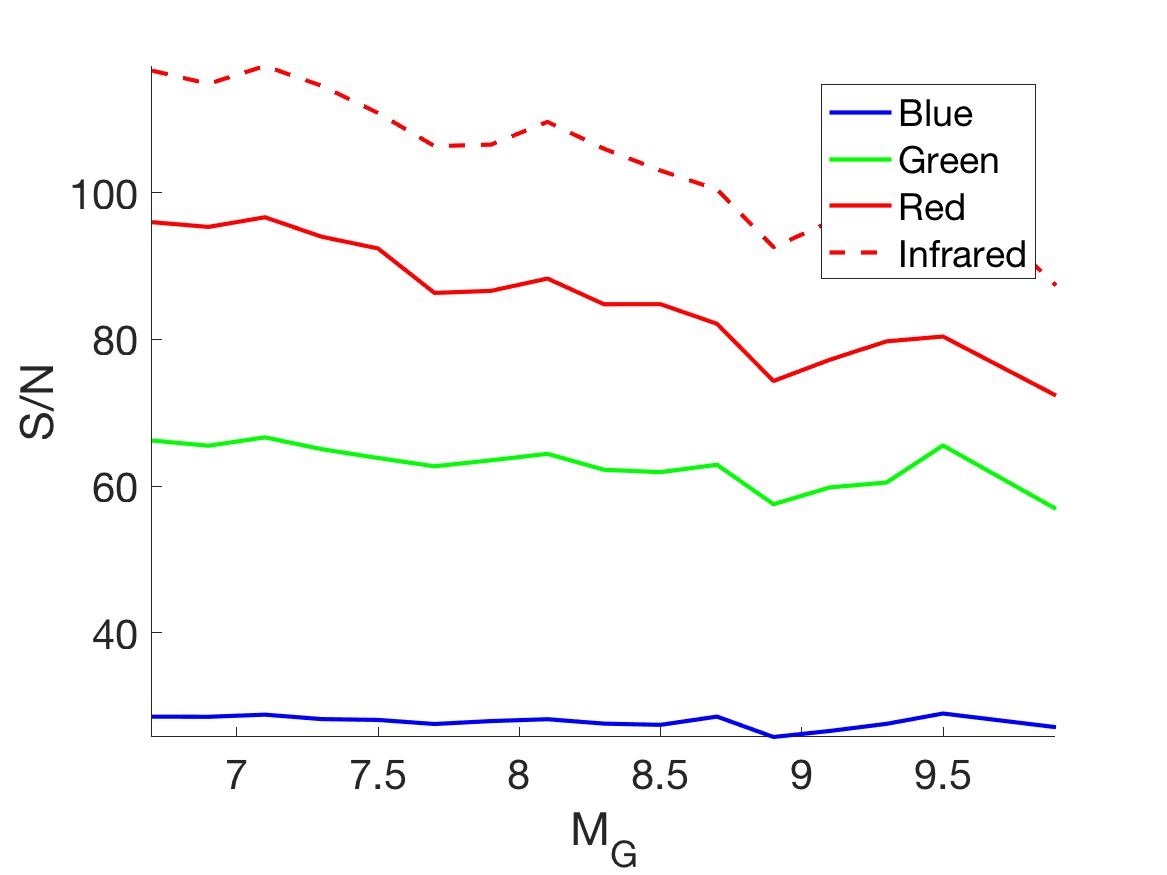
\includegraphics[width=.8\textwidth]{GALAH_SN.png}
    \caption{The mean spectroscopic signal-to-noise per pixel for each camera as a function of absolute magnitude.}
    \label{figGALAHsn_mg}
\end{figure}

The GALAH data reduction pipeline calculates and reports the signal-to-noise ratio per pixel in each camera. For each absolute magnitude bin, the signal-to-noise for each observation was used to calculate the mean value in that bin and this is plotted in Figure\,\ref{figGALAHsn_mg}. Signal-to-noise is highest for the most luminous stars and decreases as absolute magnitude increases. Also, the signal-to-noise is larger at longer wavelengths. Both of these effects are to be expected as GALAH is a magnitude-limited survey, and the peak of the flux distribution for cool stars is toward red wavelengths.\\

\begin{figure}
	\captionsetup{width=.8\textwidth}
	\subfloat[40]{\label{figpc40}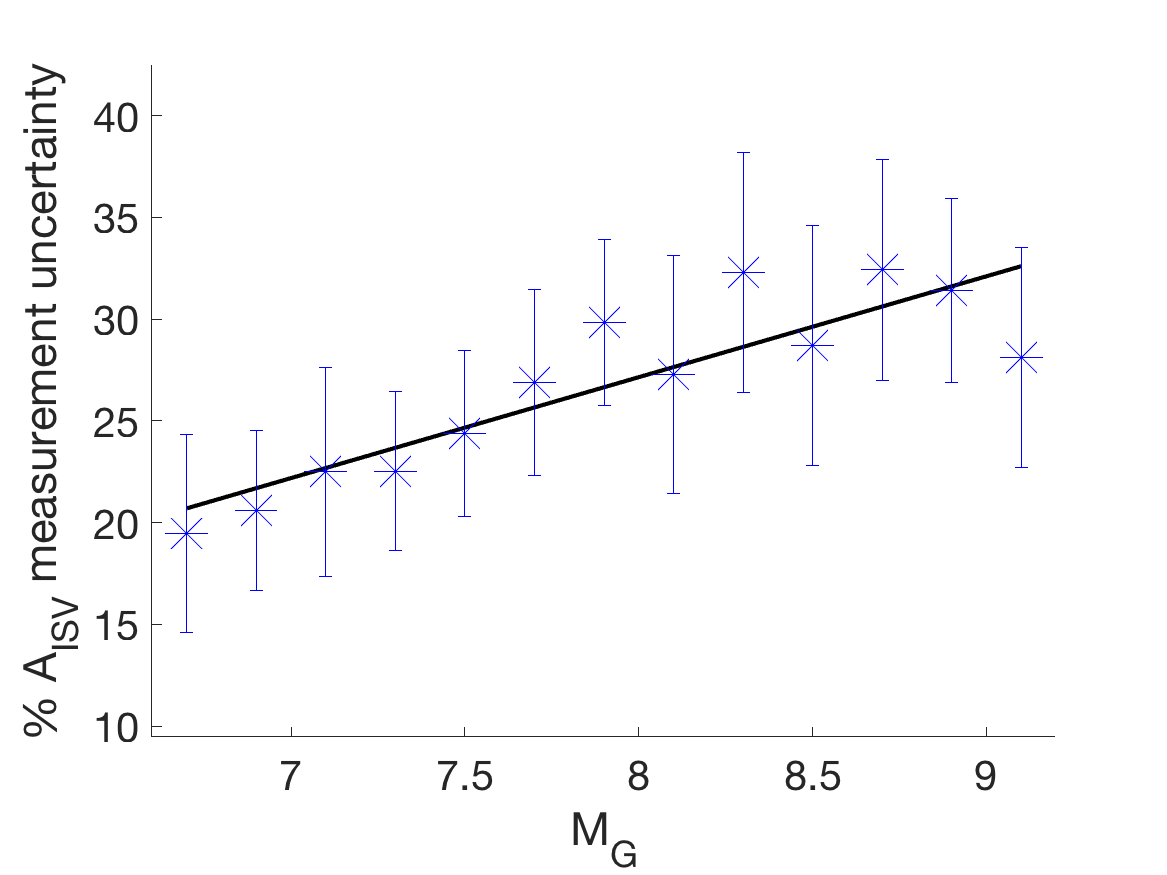
\includegraphics[width=0.5\textwidth]{GALAH_pc_err_40.png}}
    \subfloat[100]{\label{figpc100}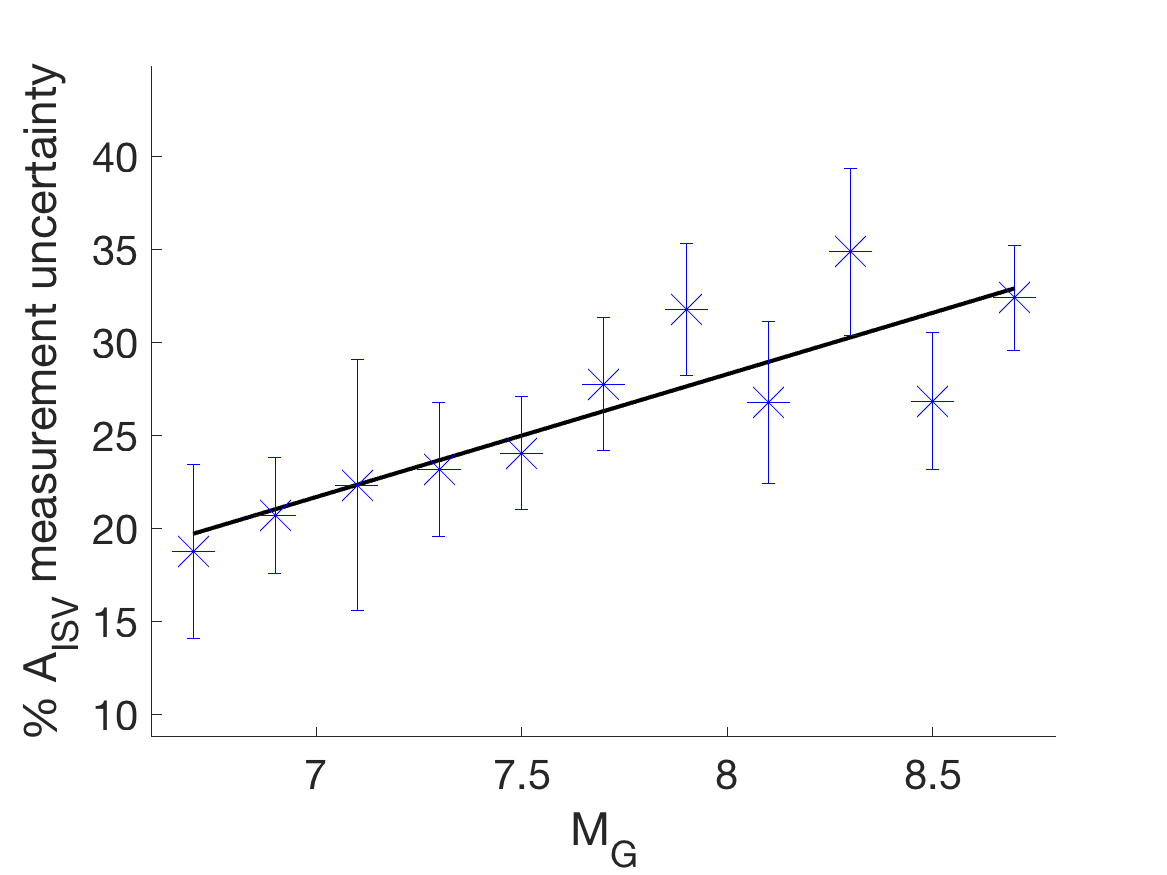
\includegraphics[width=0.5\textwidth]{GALAH_pc_err_100.png}}\\
    \subfloat[200]{\label{figpc200}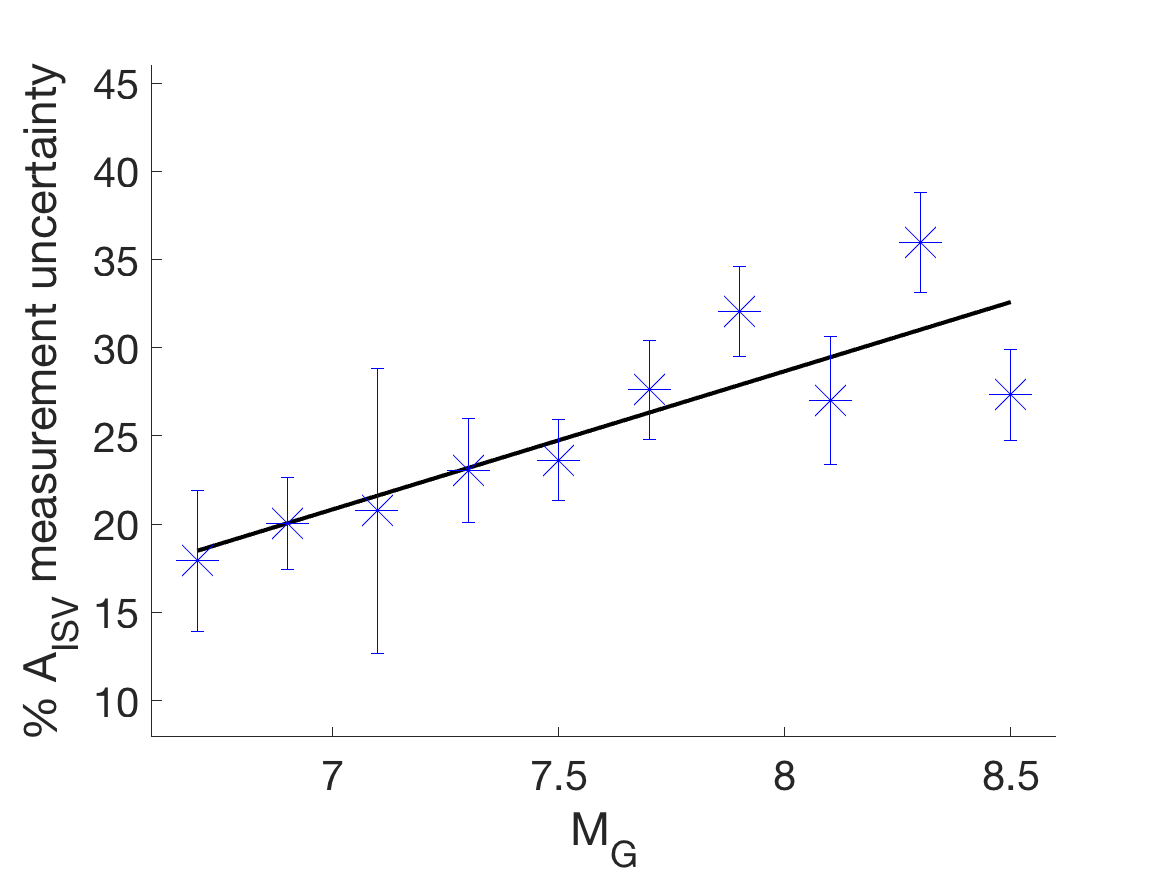
\includegraphics[width=0.5\textwidth]{GALAH_pc_err_200.png}}
    \subfloat[Comparison]{\label{figpccomp}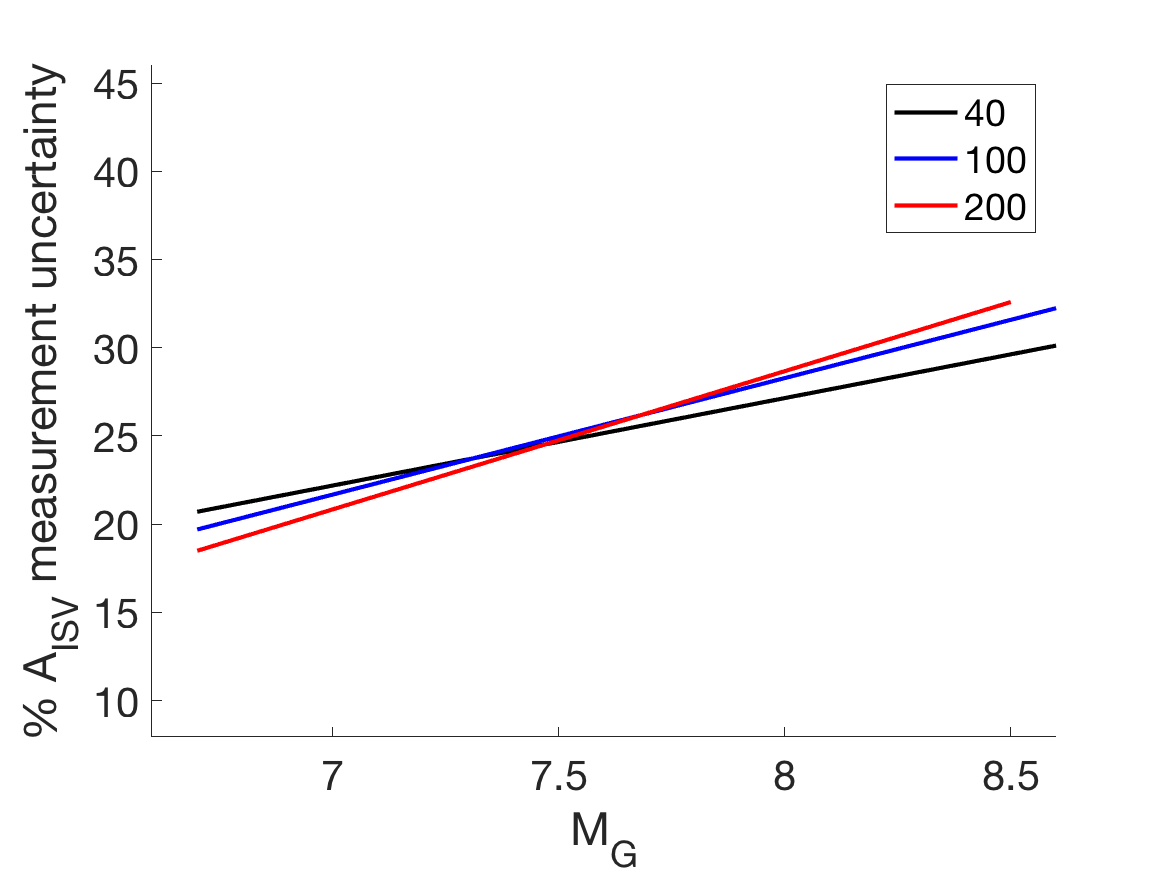
\includegraphics[width=0.5\textwidth]{GALAH_pc_err_comparison.png}}
    \caption{Figures\,\ref{figpc40}-\ref{figpc200}: Percentage measurement uncertainty as a function of absolute magnitude. Each plot presents the mean percentage uncertainty for ISV spectra produced by 40, 100, and 200 randomly selected observations in each absolute magnitude bin over 1,000 trials. The error bars for each data point present the scatter across the 1,000 trials. Figure\,\ref{figpccomp}: the linear trends from Figures\,\ref{figpc40}-\ref{figpc200}.}
    \label{figGALAHpcerr}
\end{figure}

The number of observations used to construct an ISV spectrum varies significantly with absolute magnitude, with the brightest bin containing $\sim$1,500 observations while the dimmest bin contains just 22 observations. This impacts the baseline noise, and therefore the $A_{ISV}$ measurement uncertainty. To disentangle the number of observations from the influence of absolute magnitude on the measurement uncertainty, a Monte Carlo approach was taken. ISV spectra were produced from 40 randomly selected spectra in each absolute magnitude bin, and the mean percentage measurement uncertainty of all ISV spectral lines was found. This was repeated over 1,000 trials, each time selecting a new subsample of 40 observations. The previous steps were then repeated using 100 and 200 randomly selected spectra from each absolute magnitude bin.\\

The mean percentage measurement uncertainty across the 1,000 trials for each sample size are plotted in Figures\,\ref{figpc40}-\ref{figpc200}. The first conclusion to be made is that the percentage uncertainty increases with absolute magnitude. As the signal-to-noise decreases with absolute magnitude (Figure\,\ref{figGALAHsn_mg}) this will produce more baseline noise in the ISV spectrum, and therefore a greater uncertainty in ISV spectral line intensity measurements. The second aspect to note is that while the larger sample size produces a lower percentage uncertainty at bright magnitudes, the rate of increase is also greater, producing the greatest percentage uncertainty for the dimmest stars. For 40 observations per bin, the rate of increase is 4.96\% per magnitude, with the 100 and 200 observation sample sizes increasing by 6.60\% and 7.85\% per magnitude, respectively.\\

Clearly sample size is only influential for bright stars, where the signal-to-noise is greatest. For samples of stars fainter than $M_G$\,=\,7.5, the signal-to-noise in the spectra used to construct the ISV will be the primary factor driving measurement uncertainty.\\

\subsection{Hydrogen $\alpha$}
\label{secGALAHhalpha}
\begin{figure}
    \centering
	\captionsetup{width=.8\textwidth}
	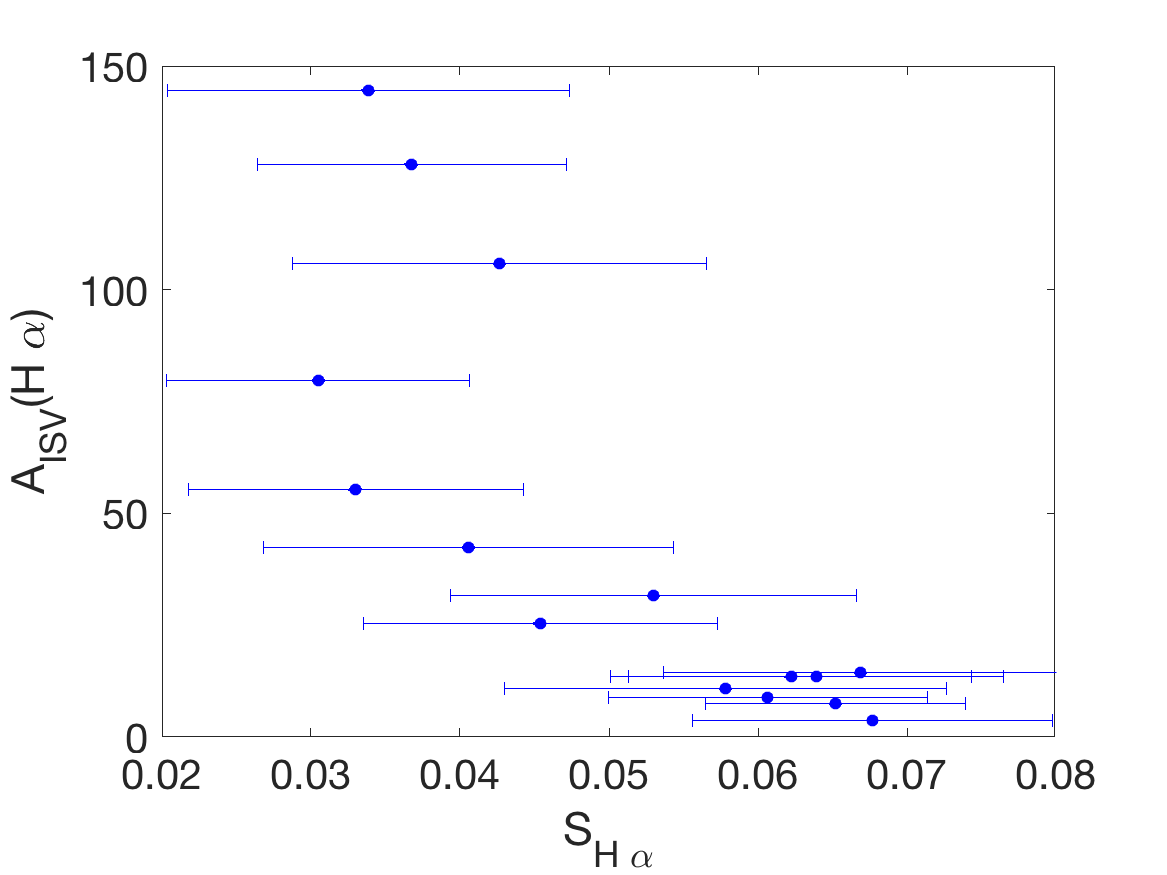
\includegraphics[width=0.8\textwidth]{GALAH_Ha_S_I.png}
	\caption{The S-index vs $A_{ISV}$ for H$\alpha$, with uncertainties, across all absolute magnitude bins. The uncertainties for $A_{ISV}$ are too small to be visible, but are generally \textless1\%.}
	\label{figGALAHhalpha}
\end{figure}

As the GALAH wavelength coverage includes the H$\alpha$ line, a direct comparison of $A_{ISV}$ to the S-index for a known chromospherically active line was possible. For each absolute magnitude bin, $A_{ISV}$ was measured for H$\alpha$ from the ISV, and the S-index for H$\alpha$ was measured from the spectra within the bin. Figure\,\ref{figGALAHhalpha} shows a comparison of the median S-index for H$\alpha$ with $A_{ISV}$ in each bin. While there is some scatter at low S$_{H\alpha}$, generally there is a clear trend towards decreasing  $A_{ISV}$ with increasing S$_{H\alpha}$. The Pearson correlation between the two metrics is P\,=\,-0.804, which confirms the inverse relationship seen in Figure\,\ref{figGALAHhalpha}. In each absolute magnitude bin, $A_{ISV}$ is measuring the variety in line strength while the median of S$_{H\alpha}$ is the typical value of line emission strength. For the more luminous K stars, $A_{ISV}$ tends to be high and S$_{H\alpha}$ is low, meaning that the typical H$\alpha$ line strength is low but it shows significant star-to-star variation. Conversely, for the less luminous stars, the median S$_{H\alpha}$ is high while $A_{ISV}$ is low, indicating that the M stars tend to have stronger H$\alpha$ with less variation between stars.

\subsection{Equivalent width}
Figures\,\ref{figGALAHew6_7}-\ref{figGALAHew9_9} compare $A_{ISV}$ against $\sigma_{EW}$ for each line in Table\,\ref{tabGALAHfreqlines} for each absolute magnitude bin, with H$\alpha$ highlighted in red and H$\beta$ in green. Please note that uncertainty bars are included, however at the scale required for all the data points, they are difficult to see in most cases. There is some correlation between $\sigma_{EW}$ and $A_{ISV}$ in each bin. The Pearson correlation (printed above each plot) is generally quite high (i.e. the majority have a value of P \textgreater 0.75), indicating that the scatter in equivalent width is proportional to the magnitude of the corresponding ISV spectral line. In some bins (e.g. $M_G$\,=\,9.3-9.5 or $M_G$\,=\,8.7-8.9), this correlation is mainly driven by the strength of H$\alpha$ compared to the other ISV spectral lines, and in some bins H$\alpha$ and H$\beta$ are decoupled. However, in the majority of bins, the correlation is strong when calculated with or without the Balmer lines.\\

\begin{figure}
	\captionsetup{width=.8\textwidth}
	\subfloat[$M_G$ = 6.7-6.9]{\label{figGALAHew6_7}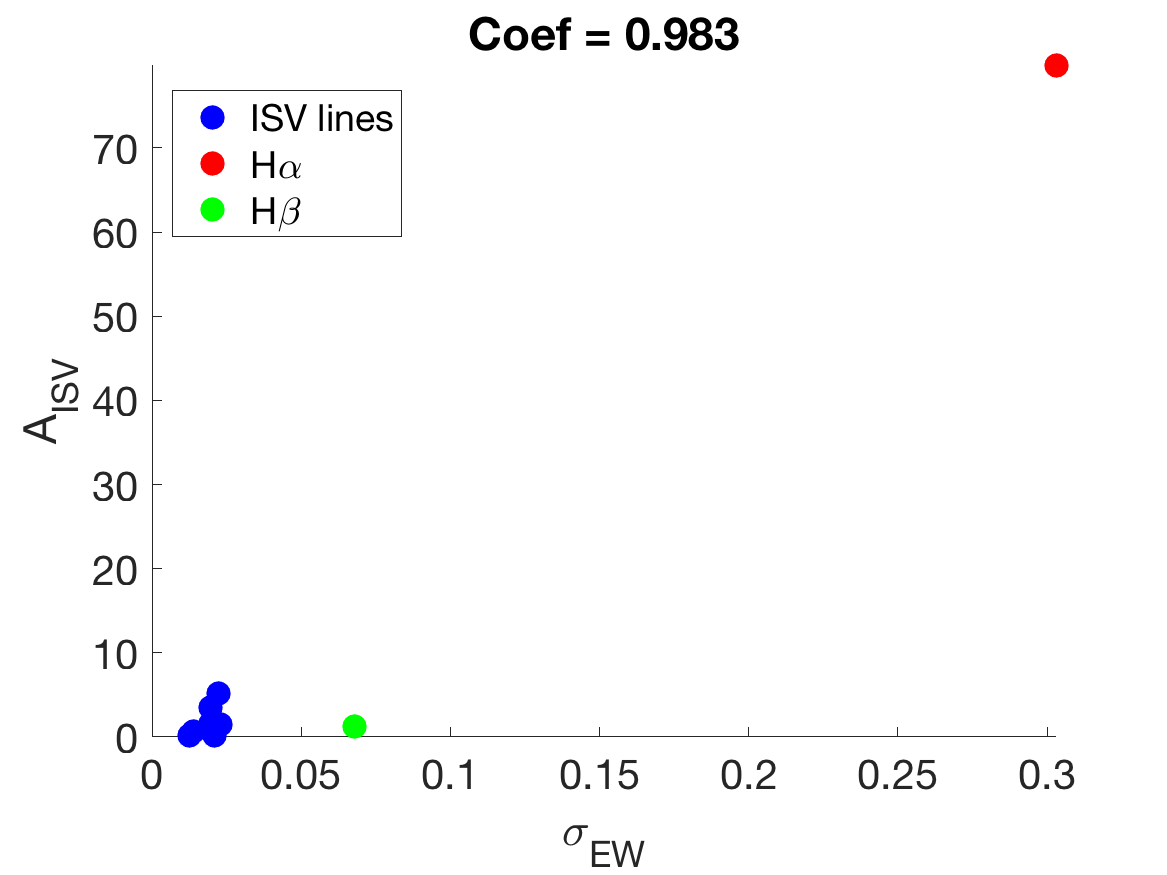
\includegraphics[width=0.5\textwidth]{GALAH_EWidth/GALAH_ISV_EW_6_7.png}}
    \subfloat[$M_G$ = 6.9-7.1]{\label{figGALAHew6_9}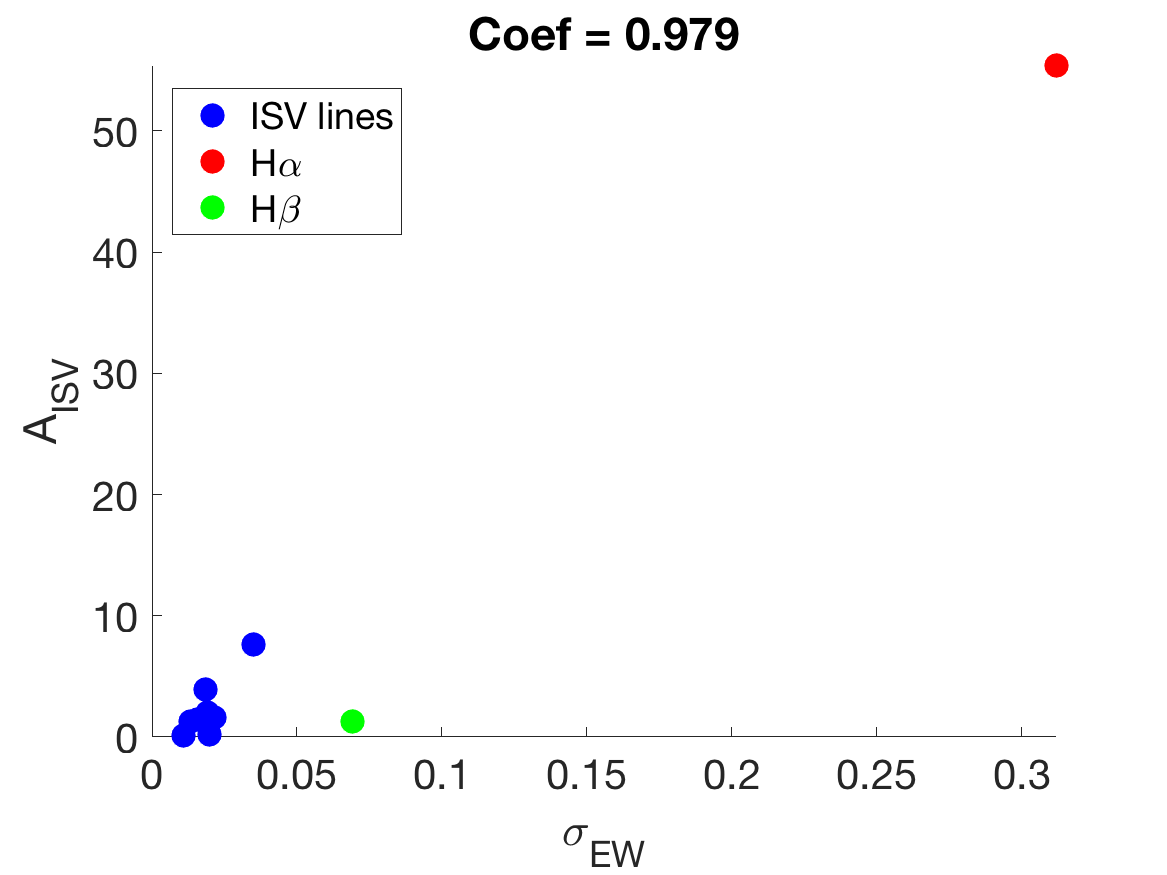
\includegraphics[width=0.5\textwidth]{GALAH_EWidth/GALAH_ISV_EW_6_9.png}}
    \caption{ISV spectral line magnitude vs scatter in spectral equivalent width for stars in the $M_G$\,=\,6.7-6.9 and 6.9-7.1 bins.}
\end{figure}
\begin{figure}
	\captionsetup{width=.8\textwidth}
	\subfloat[$M_G$ = 7.1-7.3]{\label{figGALAHew7_1}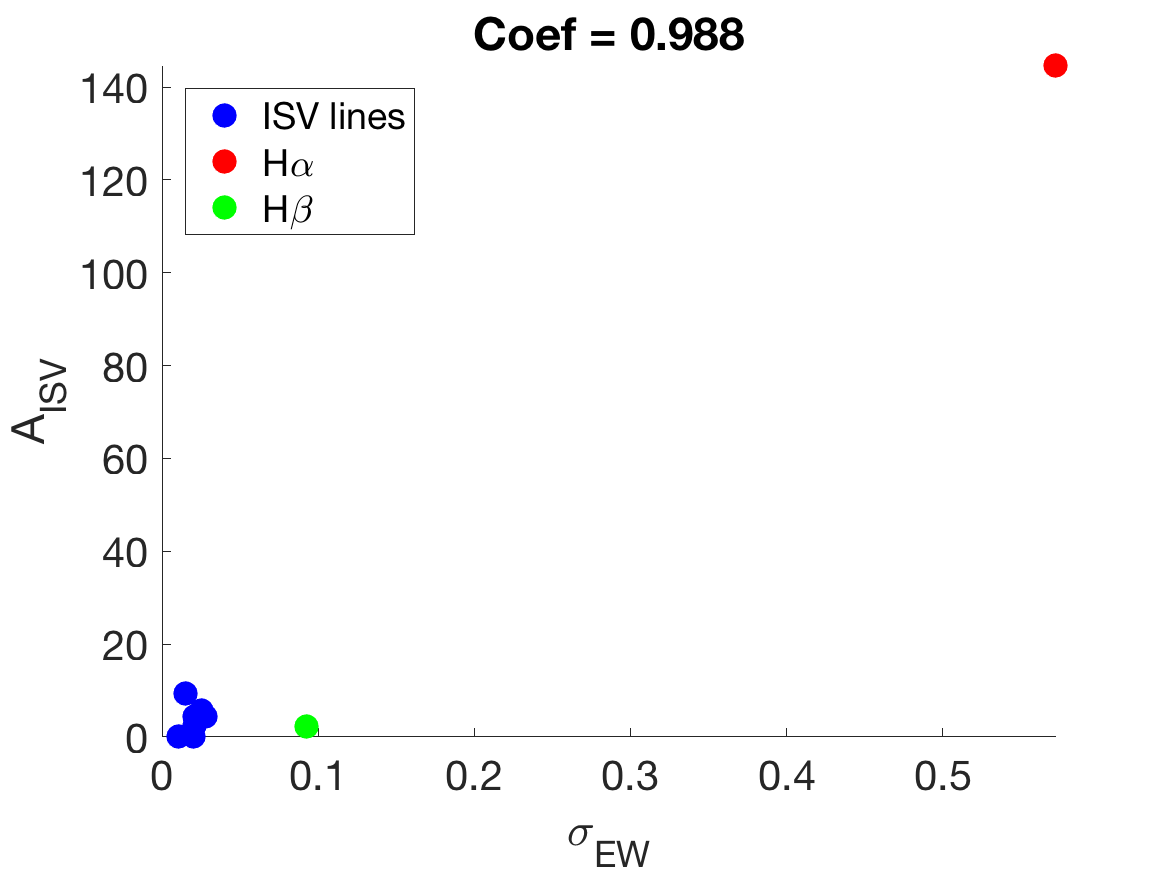
\includegraphics[width=0.5\textwidth]{GALAH_EWidth/GALAH_ISV_EW_7_1.png}}
    \subfloat[$M_G$ = 7.3-7.5]{\label{figGALAHew7_3}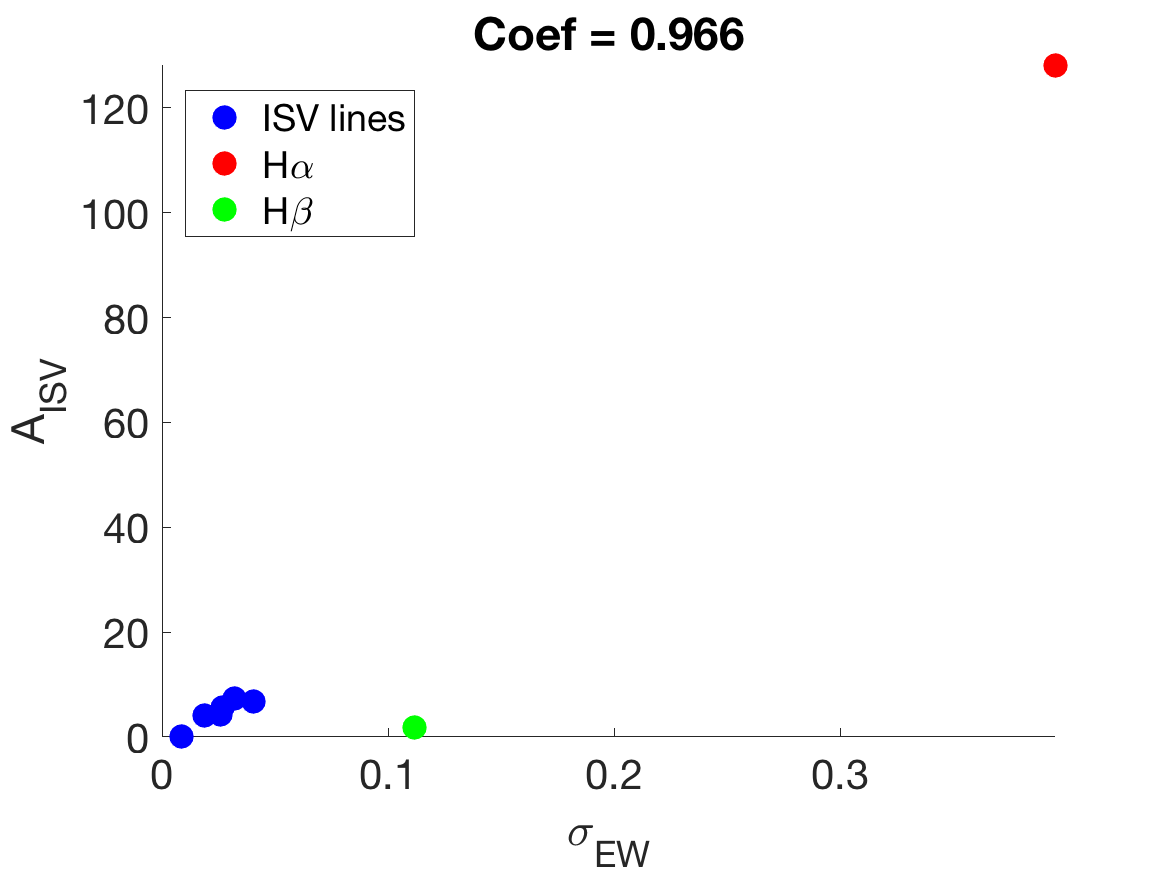
\includegraphics[width=0.5\textwidth]{GALAH_EWidth/GALAH_ISV_EW_7_3.png}}
    \caption{ISV spectral line magnitude vs scatter in spectral equivalent width for stars in the $M_G$\,=\,7.1-7.3 and 7.3-7.5 bins.}
\end{figure}
\begin{figure}
	\captionsetup{width=.8\textwidth}
	\subfloat[$M_G$ = 7.5-7.7]{\label{figGALAHew7_5}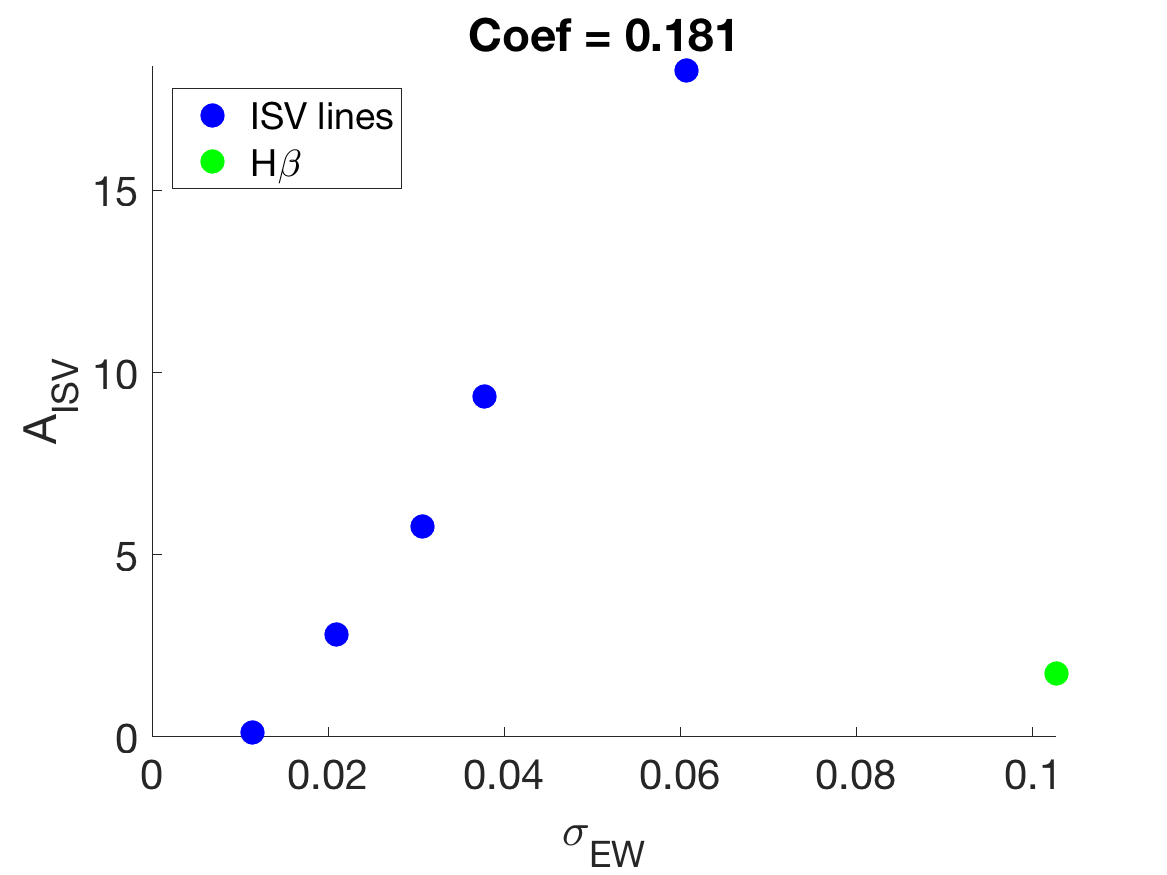
\includegraphics[width=0.5\textwidth]{GALAH_EWidth/GALAH_ISV_EW_7_5.png}}
    \subfloat[$M_G$ = 7.7-7.9]{\label{figGALAHew7_7}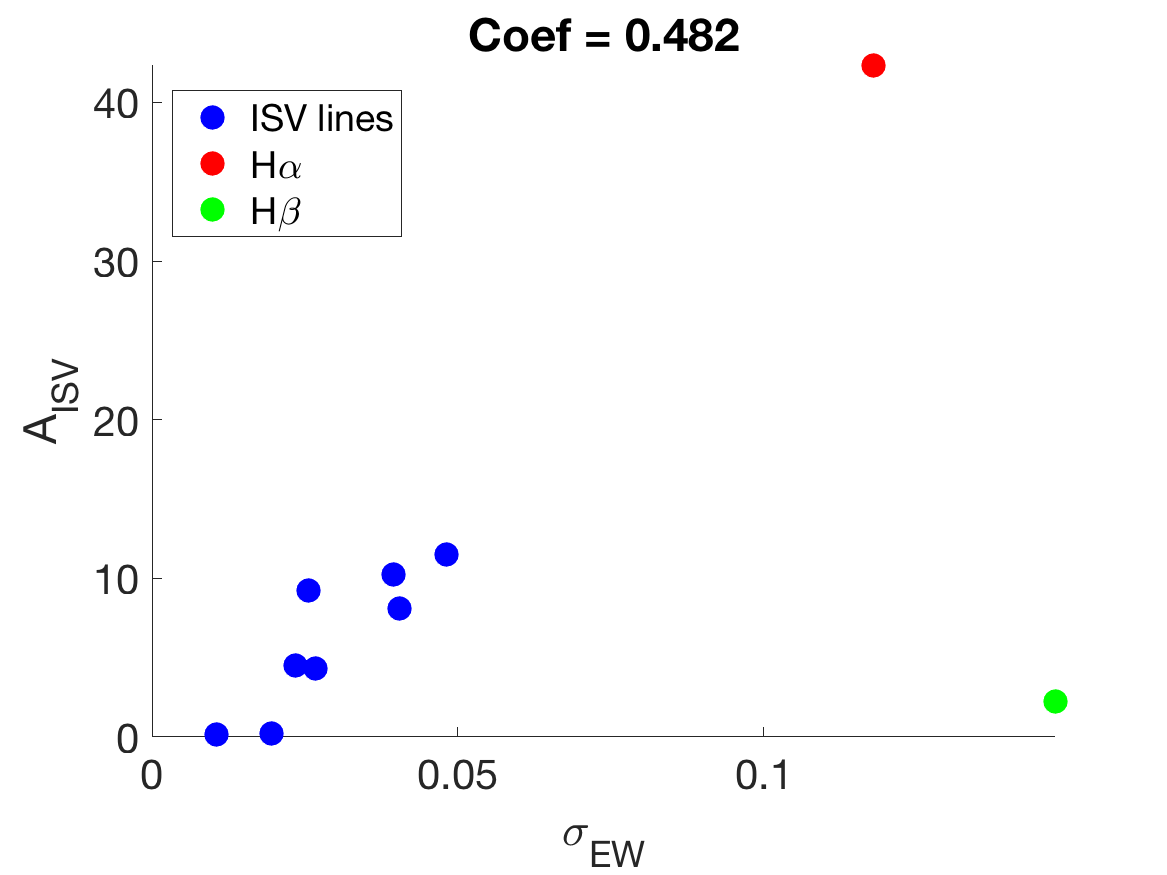
\includegraphics[width=0.5\textwidth]{GALAH_EWidth/GALAH_ISV_EW_7_7.png}}
    \caption{ISV spectral line magnitude vs scatter in spectral equivalent width for stars in the $M_G$\,=\,7.5-7.7 and 7.7-7.9 bins.}
\end{figure}
\begin{figure}
	\captionsetup{width=.8\textwidth}
	\subfloat[$M_G$ = 7.9-8.1]{\label{figGALAHew7_9}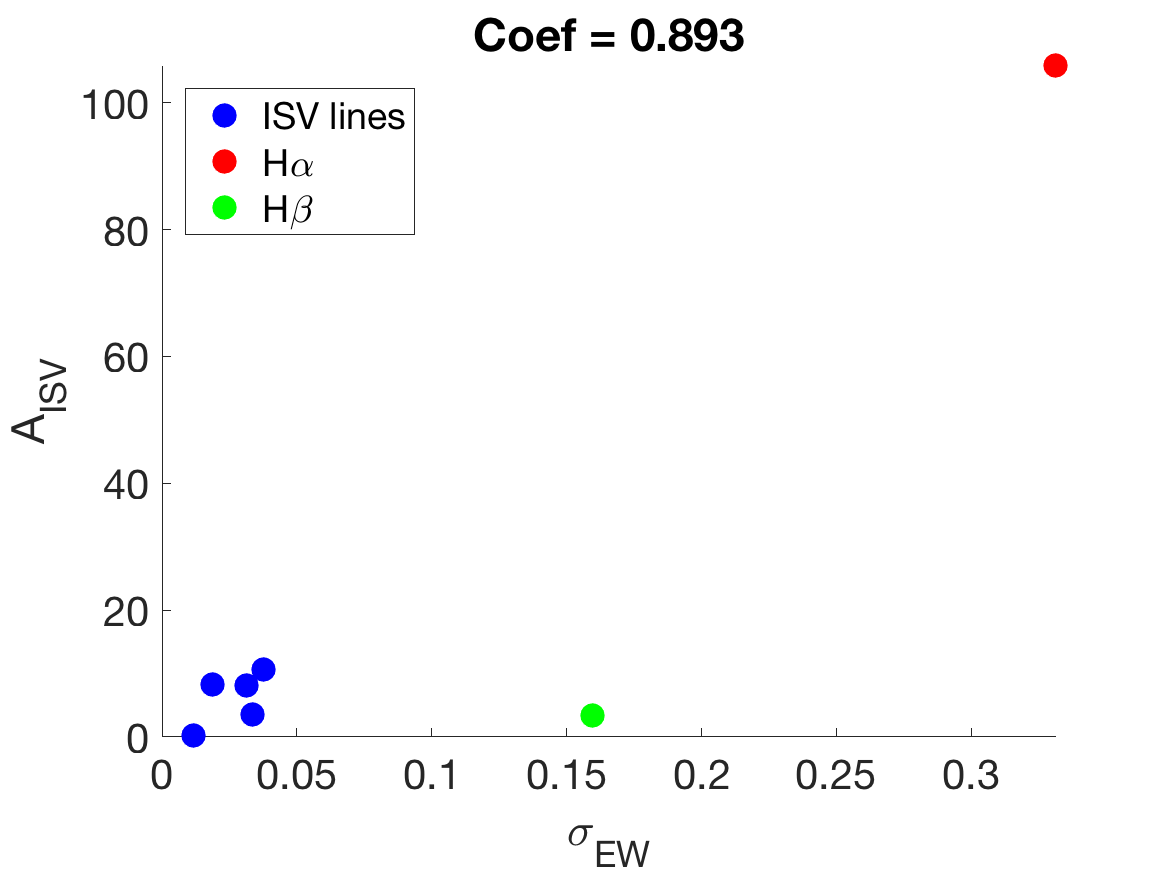
\includegraphics[width=0.5\textwidth]{GALAH_EWidth/GALAH_ISV_EW_7_9.png}}
    \subfloat[$M_G$ = 8.1-8.3]{\label{figGALAHew8_1}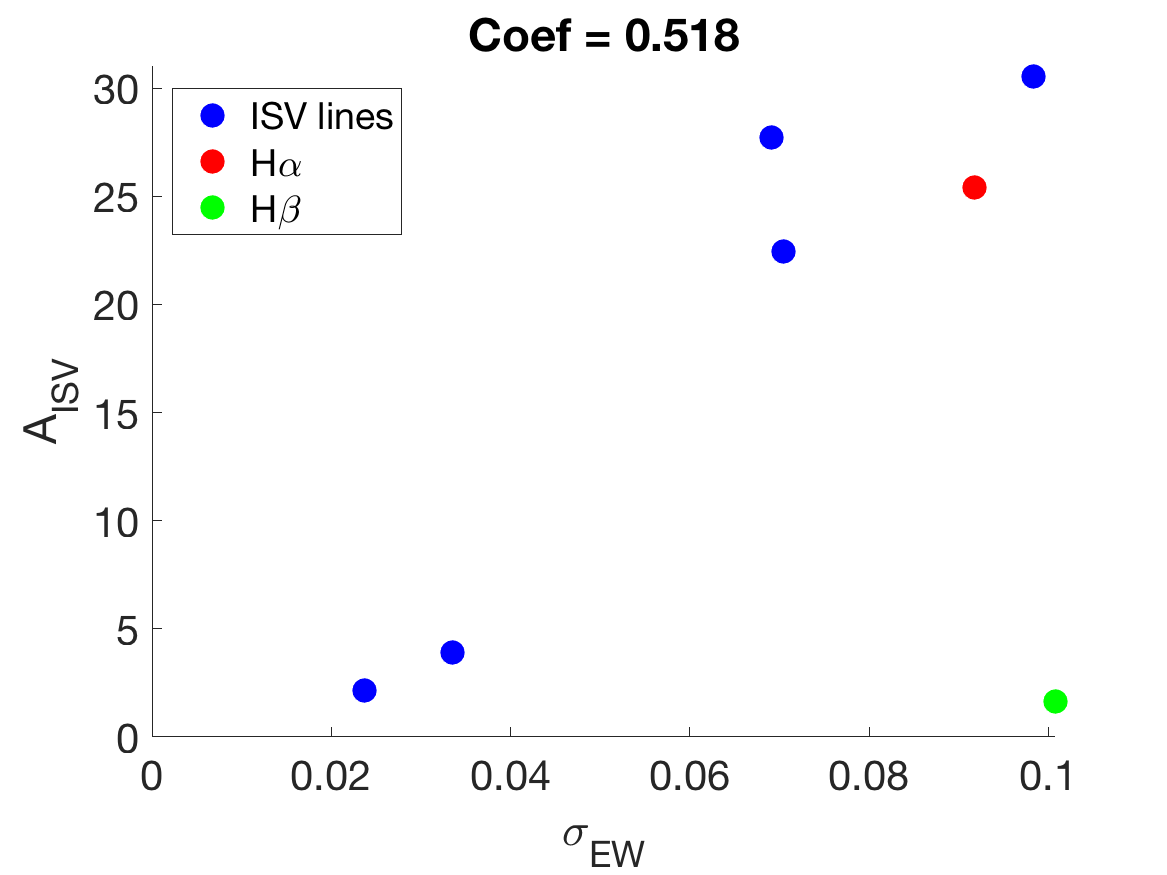
\includegraphics[width=0.5\textwidth]{GALAH_EWidth/GALAH_ISV_EW_8_1.png}}
    \caption{ISV spectral line magnitude vs scatter in spectral equivalent width for stars in the $M_G$\,=\,7.9-8.1 and 8.1-8.3 bins.}
\end{figure}
\begin{figure}
	\captionsetup{width=.8\textwidth}
	\subfloat[$M_G$ = 8.3-8.5]{\label{figGALAHew8_3}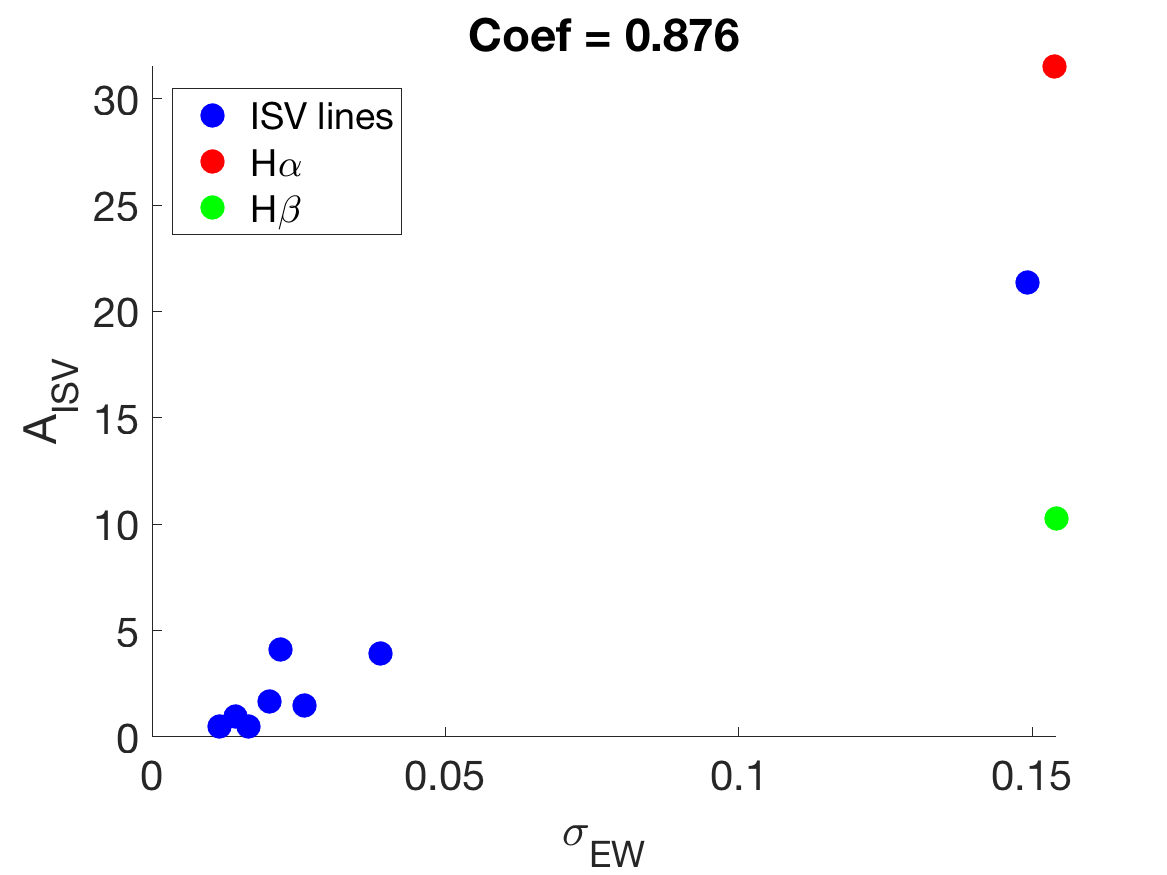
\includegraphics[width=0.5\textwidth]{GALAH_EWidth/GALAH_ISV_EW_8_3.png}}
    \subfloat[$M_G$ = 8.5-8.7]{\label{figGALAHew8_5}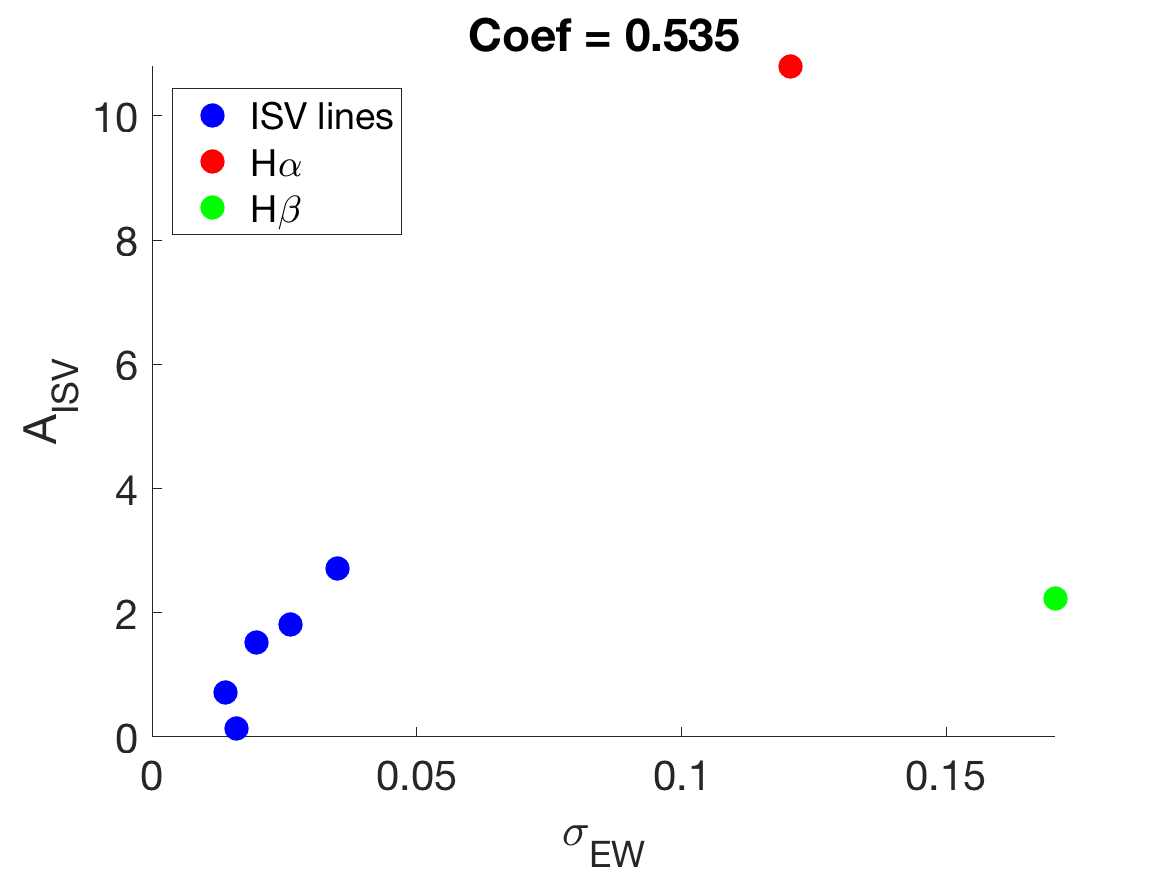
\includegraphics[width=0.5\textwidth]{GALAH_EWidth/GALAH_ISV_EW_8_5.png}}
    \caption{ISV spectral line magnitude vs scatter in spectral equivalent width for stars in the $M_G$\,=\,8.3-8.5 and 8.5-8.7 bins.}
\end{figure}
\begin{figure}
	\captionsetup{width=.8\textwidth}
	\subfloat[$M_G$ = 8.7-8.9]{\label{figGALAHew8_7}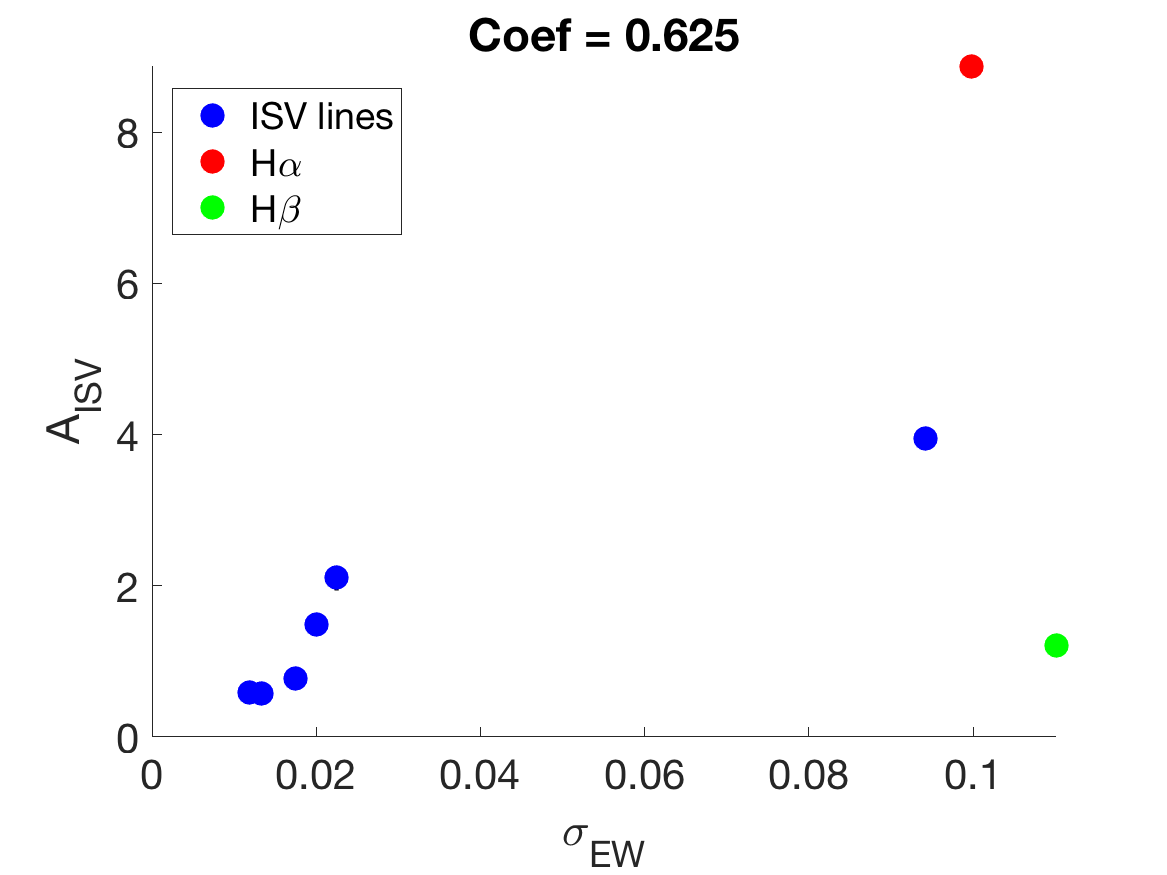
\includegraphics[width=0.5\textwidth]{GALAH_EWidth/GALAH_ISV_EW_8_7.png}}
    \subfloat[$M_G$ = 8.9-9.1]{\label{figGALAHew8_9}\includegraphics[width=0.5\textwidth]{GALAH_EWidth/GALAH_ISV_EW_8_9.png}}
    \caption{ISV spectral line magnitude vs scatter in spectral equivalent width for stars in the $M_G$\,=\,8.7-8.9 and 8.9-9.1 bins.}
\end{figure}
\begin{figure}
	\captionsetup{width=.8\textwidth}
	\subfloat[$M_G$ = 9.1-9.3]{\label{figGALAHew9_1}\includegraphics[width=0.5\textwidth]{GALAH_EWidth/GALAH_ISV_EW_9_1.png}}
    \subfloat[$M_G$ = 9.3-9.5]{\label{figGALAHew9_3}\includegraphics[width=0.5\textwidth]{GALAH_EWidth/GALAH_ISV_EW_9_3.png}}
    \caption{ISV spectral line magnitude vs scatter in spectral equivalent width for stars in the $M_G$\,=\,9.1-9.3 and 9.3-9.5 bins.}
\end{figure}
\begin{figure}
	\captionsetup{width=.8\textwidth}
	\subfloat[$M_G$ = 9.5-9.7]{\label{figGALAHew9_5}\includegraphics[width=0.5\textwidth]{GALAH_EWidth/GALAH_ISV_EW_9_5.png}}
    \subfloat[$M_G$ = 9.9-10.1]{\label{figGALAHew9_9}\includegraphics[width=0.5\textwidth]{GALAH_EWidth/GALAH_ISV_EW_9_9.png}}
    \caption{ISV spectral line magnitude vs scatter in spectral equivalent width for stars in the $M_G$\,=\,9.5-9.7 and 9.9-10.1 bins.}
\end{figure}

Combining the measurements from all absolute magnitude bins into Figure\,\ref{figGALAH_AISV_EW}, a line of best fit can be obtained that will allow for an estimation of the scatter in the equivalent width of a line over multiple observations by producing an ISV spectrum and measuring the $A_{ISV}$ of the line. The data produced a relationship of $\sigma_{EW} = 0.00329\,A_{ISV} + 0.038$.

\begin{figure}
    \centering
    \includegraphics[width=.8\textwidth]{GALAH_AISV_EW.png}
    \caption{The $A_{ISV}$ and $\sigma_{EW}$ measurements for all lines identified in the GALAH ISV spectra. The black line is a linear regression best fit used to estimate the relationship between the two measurements. The red lines are 2 times the standard error of the linear regression, which corresponds to the 95.4\% confidence intervals for the fit.}
    \label{figGALAH_AISV_EW}
\end{figure}

\subsection{Line variability and elemental abundances}
\label{secGALAHabundance}
The equivalent width of a spectral line is used to determine 
the abundance of the element that produced the line, along with information about the conditions in the stellar photosphere. The uncertainty in abundance measurements comes from uncertainties in stellar parameters, noise in the spectra, and the scatter between the abundance measurements from each line, if multiple lines are measured for a particular species. As discussed in the previous section, there is a correlation between the scatter of the equivalent width of a line among all of the stars in one of the absolute magnitude bins and the strength of the corresponding ISV spectral line. If line variability affects the equivalent width, it will therefore influence any abundance measurements made with that equivalent width.\\

GALAH has measured abundances for all of the individual spectral lines in Table\,\ref{tabGALAHfreqlines}, which have been identified as variable from this ISV analysis. While K-dwarf abundances are reasonably robust, the cool temperatures of M-dwarfs mean that the stellar parameters and abundances derived for them by GALAH are uncertain, so only the K-dwarfs in the sample were used for this analysis. The K-dwarf subsample has an effective temperature range of 3,000\,-\,5,700 K. Both these limits are outside that expected for K-dwarfs (see Table 2.2). However, the majority of the sample is within the expected temperature range. The 16th, 50th, and 84th percentiles of the temperatures for the K-dwarf sample are 3903\,K, 4432\,K, and 4636\,K respectively. The reason there are such extreme outliers present in the sample can be attributed to the uncertainty in the effective temperatures of the stars, and the expected presence of non-K-dwarfs (contamination).\\ 

The GALAH data reduction pipeline determines the effective temperature of a star by $\chi^2$ optimisation of the observed spectra with a synthetic spectrum, using the Spectroscopy Made Easy (SME) package\citep{1996Valenti}. The pipeline selects forty-six wavelength regions, normalises them using a linear to the data, and obtains initial estimates for T$_{eff}$, [Fe/H], and vsin(i). These values are then used to re-normalise the spectra and iterate until the fractional change in $\chi^2$ is \textless0.001. The uncertainties on these stellar parameters are obtained from adding the accuracy and precision in quadrature (see Section 4 of \citealt{2021Buder} for details on the accuracy and precision). For spectra with a SN of 40 per pixel, the GALAH team expects a typical uncertainty for the temperature of 83\,K. Cooler stars will produce spectra with lower SN, resulting in a greater mean temperature uncertainty. The K-dwarf sample was subdivided into bins containing the stars too cool to be a K-dwarf (T$_{eff}$\,\textless\,3900\,K), those too hot to be a K-dwarf (T$_{eff}$\,\textgreater\,4600\,K), and the stars within in the K-dwarf temperature range (3900\,K\,\textless\,T$_{eff}$\,\textless\,4600\,K). The distribution of effective temperatures for these bins showed general agreement, mean temperatures differing by \textless3\,K, and an overall mean uncertainty of the effective temperatures of 96\,K. This indicates that the K-dwarf sample, regardless of temperature range, contains slightly greater uncertainties than the expected mean. However, this does not fully explain the presence of the stars in the sample too hot or too cold to be K-dwarfs. The K-dwarf subsample was derived solely from photometric properties. The scatter in the relationship between those photometric properties and underlying photospheric temperature, combined with the relevant photometric measurement uncertainties, means that there will be some non-K-dwarf contamination of the resulting photometrically-selected K-dwarf sample.\\ 

To ensure that the abundance measurements were reliable, only abundances with a quality flag of 0 were used. To ensure the abundances came from stars with sufficient signal-to-noise, the subsample was further limited to the brightest absolute magnitude bin of $M_G$\,=\,6.7-6.9.\\

Many of the species for which GALAH reports abundances have multiple transitions in the line list. An overall abundance for a species is taken as the weighted mean abundance across these lines. If stellar activity is driving significant equivalent width variability in a particular line, that will increase the scatter in the individual spectral line abundances and therefore the uncertainty on the overall abundance for that element. It is therefore important to identify ISV spectral lines as a way to improve the precision of derived abundances. At the same time, the ISV spectra calculated from the GALAH sample are constructed from the spectra of many stars, and an abundance range in that set of stars could also create apparent ISV features for lines where the equivalent width is particularly sensitive to abundance in the temperature range under consideration. In understanding the importance of ISV lines for GALAH abundances, these two effects need to separated.\\

\begin{figure}
    \centering
    \includegraphics[width=.8\textwidth]{GALAH_Ti_abundance.png}
    \caption{Plots of the GALAH measured abundances for the 15 titanium lines in the GALAH line list. (Top) Mean abundances for the K-dwarfs in the brightest absolute magnitude bin. The black horizontal line represents the mean of the overall [Ti/Fe] abundance. (Bottom) The standard deviation of the K-dwarf abundance measurements for the titanium lines. The red points highlight the three titanium lines that vary according to ISV analysis, and the black horizontal line represents the scatter in the overall [Ti/Fe] abundance in this bin.}
    \label{figGALAHabundance_ti}
\end{figure}

Investigation of the relative impact of these two effects for the stars in the GALAH sample can be done by comparing the abundances measured from the lines that show strong ISV against lines of the same species that do not. As an example, the GALAH line list contains 15 titanium lines with abundance measurements, and 3 of them have been identified in the ISV spectra as strongly varying - 4781.71\hbox{\AA}, 5866.45\hbox{\AA}, and 7852.68\hbox{\AA}. The vanadium line at 4831.65\hbox{\AA} was the only one of the three vanadium lines in the GALAH line list that was found to vary strongly in ISV. The remaining lines in Table\,\ref{tabGALAHfreqlines} comprise the entirety of their species in the GALAH line list, meaning there are no non-variable lines to compare to the `strong' ISV lines. The abundances of all the Ti and V lines for this subsample were obtained from the GALAH DR3 catalogue, and the mean and standard deviation of the overall [Ti/Fe] and [V/Fe] abundances were determined.\\

\begin{figure}
    \centering
    \includegraphics[width=.8\textwidth]{GALAH_V_abundance.png}
    \caption{Plots of the GALAH measured abundances for each vanadium line in the line list. (Top) Mean abundances for the K-dwarfs in the brightest absolute magnitude bin. The black horizontal line represents the mean of the overall [V/Fe] abundance. (Bottom) The scatter in the abundance measurements for the vanadium lines. The red points highlight the vanadium lines that varied according to ISV analysis, and the black horizontal line represents the standard deviation in the overall [V/Fe] abundance.}
    \label{figGALAHabundance_v}
\end{figure}

Figure\,\ref{figGALAHabundance_ti} plots the mean per-line abundance in the upper panel, and the scatter about the mean in the lower panel, for all 15 titanium lines in the line list, while Figure\,\ref{figGALAHabundance_v} shows the same information for the 3 vanadium lines. The active ISV lines are highlighted in red. The mean of the overall [Ti/Fe] and [V/Fe] abundances is plotted with black dashed lines in the upper panels, and the standard deviation in the overall abundance is shown with black dashed lines in the lower panels. Neither element shows an obvious relationship between spectral variability as captured by ISV and the mean value of the per-line abundance. \\

For titanium, two of the three ISV lines show a larger scatter in per-line abundance than the non-ISV lines, but the third is consistent with the non-ISV lines and with the scatter in overall [Ti/Fe] abundance. The per-line abundances for the three ISV lines are also consistent with the abundances from the non-ISV lines. This indicates that the spectroscopic variability we identify using ISV does not correspond to inaccurate abundance determinations, but it may limit the precision of those abundances by introducing scatter to the per-line abundances. The vanadium line at 4831.65\hbox{\AA} is above the median [V/Fe] abundance, and the scatter in its abundance is quite consistent with the scatter in the overall [V/Fe] in this sample. As there are only three vanadium lines to consider, there is little that can be confidently concluded from this. Overall there is insufficient evidence to prove that stellar activity is the source of the variation in these abundances.\\

\section{Conclusion}
\label{secGALAHconclusion}
Spectra and photometry were compiled for a sample of 6,440 K- and M- dwarfs using a photometric selection on the GALAH survey data. Given the difference in data characteristics from the HARPS data in Chapter\,\ref{chapISV}, a number of modifications to the method were required. The stars were divided 
into 16 narrow bins in absolute magnitude, and ISV spectra were calculated for each of the four channels of HERMES data, in each bin. The large number of observations per bin produced an ISV spectrum with a fairly low baseline noise compared to the ISV from HARPS spectra, creating a clear separation between significant ISV lines and the noise. However, since the HERMES spectrograph has a lower resolution than HARPS, blending between strong nearby ISV lines can cause difficulty in measuring their strengths.\\

As a tool to identify the spectral features responsible for significant ISV lines, the line list compiled by GALAH for abundance analysis, was used for this work. Ten lines from the GALAH line list were found to vary across at least 5 absolute magnitude bins. In many of the magnitude bins, the ISV strength in these ten lines was found to correlate significantly with the scatter in equivalent width of that line across the stars in the bin. A relationship was determined between the two measurements which can be used as a tool to estimate the expected scatter in equivalent width measurements for a line using the strength of the corresponding ISV spectral line. The scatter in equivalent width is related to the ISV spectral line magnitude by the relationship $\sigma_{EW} = 0.00329\,A_{ISV} + 0.038$.\\

The strengths of ISV spectral lines were found to change as a function of absolute magnitude. Generally there was a change in ISV line strength between K-dwarfs and M-dwarfs, but for a few lines the ISV strength was low for most bins but high at the K-M transition. The measurement uncertainties on $A_{ISV}$ were fairly insensitive to absolute magnitude, and so the percentage uncertainty percentage uncertainty behaved as the inverse of the ISV strength, rising when the ISV line strength decreased, and decreasing when the ISV line grew stronger.\\ 

Further investigation of the percentage uncertainty on $A_{ISV}$ found that while the number of observations used to create an ISV spectrum has a strong influence on the measurement uncertainty for the more luminous stars, the spectroscopic signal-to-noise plays a dominant role for ISV spectra produced from low-luminosity stars. The rate of increase per absolute magnitude was found to be around 5-7\% per magnitude. Overall, ensuring an ISV is produced from high signal-to-noise spectra is the highest priority to ensure the measurement uncertainty is kept at a minimum.\\

We find an inverse relationship between the ISV metric for H$\alpha$ in each absolute magnitude bin to the median of the index S$_{H\alpha}$ in each bin. This indicates that the cooler stars have more consistent H$\alpha$ line strengths, while the warmer stars tend to have weaker H$\alpha$ but more star-to-star variability. We also find that there tends to be more scatter in the abundances determined from ISV lines than from non-ISV lines, but the set of lines and elements available for this analysis is limited. The ISV method shows promise for identifying problematic spectral lines that may influence abundance measurements for active stars. As abundances are typically measured from multiple spectral lines, removing potentially variable lines from consideration may produce a more reliable measurement.